\documentclass[11pt,twocolumn]{article}
\usepackage{fontspec}
\usepackage{amsmath,amssymb,amsthm}
\usepackage{booktabs}
\usepackage{array}
\usepackage{graphicx}
\usepackage[margin=0.85in]{geometry}
\usepackage[authoryear,round]{natbib}
\usepackage{caption}
\usepackage{microtype}
\PassOptionsToPackage{hidelinks}{hyperref}
\usepackage{doi}
\DeclareMathOperator{\atan}{atan}
% Theorem-like environments with manual (paper-faithful) numbering
\newtheoremstyle{gttdef}{8pt}{8pt}{\normalfont}{}{\bfseries}{.}{0.5em}{\thmnote{#3}}
\theoremstyle{gttdef}
\newtheorem*{gttdef}{x}
\newtheoremstyle{gttplain}{8pt}{8pt}{\itshape}{}{\bfseries}{.}{0.5em}{\thmnote{#3}}
\theoremstyle{gttplain}
\newtheorem*{gttplain}{x}
\setlength{\emergencystretch}{2em}

\title{The General Theory of Trust: A Multiscale Formalism\\ for Expectation--Validation Dynamics}
\author{Devon Shigaki~(ORCID: 0009-0003-8977-8010)\\
\small The FreshCredit Lab --- Independent Research\\
\small Correspondence: freshcredit.xyz}
\date{}

% --- Float-page layout tuning: reduce white bands on float-dense pages ---
\renewcommand{\topfraction}{0.85}
\renewcommand{\bottomfraction}{0.70}
\renewcommand{\textfraction}{0.10}
\renewcommand{\floatpagefraction}{0.60}
\renewcommand{\dbltopfraction}{0.80}
\renewcommand{\dblfloatpagefraction}{0.55}
\setcounter{topnumber}{3}
\setcounter{bottomnumber}{2}
\setcounter{totalnumber}{5}
\raggedbottom


\begin{document}
\twocolumn[{\begin{@twocolumnfalse}
\maketitle
\begin{abstract}
Trust is typically treated as an attitude, a disposition, or a social lubricant --- constructs that resist measurement and resist unification across scales. This paper proposes the General Theory of Trust (GTT): trust is a measurable dynamical quantity defined by the relationship between an agent's expectations $(E)$ and the validations $(V)$ returned by its environment. We formalize trust as a five-component vector $T$ = [D, O, C, A, S] (Expectation, Validation, Recognition, Activation, Stabilization), whose stabilization component obeys the update law $\Delta S_t = \lambda(V_t - E_t)$ --- the Rescorla -- Wagner delta rule applied to trust as the state variable --- with the alignment state $E = V$ a Lyapunov-stable line of fixed points whose transverse contraction rate is the corrective bandwidth $\mu$ (phase volumes contract uniformly at rate $\mu;$ no divergence-based critical point is posited). A Mathematical Development section assembles the theory's machinery from established formalisms: the Fisher -- Rao information metric on the simplex of normalized stage-activity profiles (textbook result, derived for self-containment [STANDARD]); Lyapunov stability of the alignment fixed point [STANDARD]; a stochastic Langevin/Fokker -- Planck extension with closed-form stationary distribution [STANDARD]; an observation-dependent dissipation model in which measurement salience modulates the mismatch dynamics, with stationary variance $\sigma^{2}/(2(\mu+\psi))$ and a dissipation-floor slowing signature verified in silico [DERIVED + SIMULATION]; and a Kuramoto-type collective phase transition stated as a formal analogy whose critical coupling is a mean-field reference value, not a numerical prediction (labeled [ANALOGY]). A measurement-theoretic analysis separates four distinct senses of ``measurement'' in the theory; the quantum-decoherence correspondence is presented strictly as a labeled structural homology carrying zero inferential load (Section 3.5). We review convergent evidence across behavioral genetics, evolutionary game theory, predictive-processing neuroscience, and economic institutions, with statistics verified against their primary sources, and we position the theory explicitly against the trust-measurement canon (Berg et al., 1995; Glaeser et al., 2000; Johnson \& Mislin, 2011; Sapienza et al., 2013) and the learning-theory lineage it descends from (Rescorla \& Wagner, 1972; Sutton, 1988; Sutton \& Barto, 2018). A pre-registered empirical program (OSF registration) --- implemented through the companion measurement protocol's infrastructure --- is specified, including state-space (Kalman/EM) and Bayesian hierarchical estimators for the trust-sensitivity coefficient $\lambda.$ The population mean is pre-registered as the target $\mu_\lambda = 0.61$ inside an equivalence corridor [0.46, 0.76] whose half-width is a pre-registered smallest effect size of interest (SESOI), far coarser than the estimator's demonstrated recovery error --- a target hypothesis, not an obtained result and not a derived constant --- together with a falsifiable closed-loop consequence: at $\lambda = 0.61$ the trust dynamics are underdamped and ring after betrayal events with period $\approx 7.2$ steps under the minimal one-step loop closure $E_{t+1} = S_t$ (the period drifts $7.2 \to 17.7$ steps across smoothing closures and vanishes under zero-delay closure, \S{}6; tests must verify the closure or joint-fit $(\lambda, \alpha)$) (predicted 7.17; the recurrence's roots are the prediction, so the in-silico 7.15 is an implementation check, not corroboration). One vector state and update law, instantiated at three levels: the GTT vector is instantiated biologically through a five-channel neuromodulatory architecture and behaviorally through a domain-agnostic trust-measurement protocol (companion preprints deposited at OSF; the first application, to finance, is specified separately).
\end{abstract}
\smallskip\noindent \textbf{Keywords:} trust; information geometry; Fisher metric; predictive processing; Rescorla -- Wagner learning; Kuramoto model; measurement theory; evolutionary game theory
\bigskip
\end{@twocolumnfalse}}]
\medskip
\noindent\textbf{Contents}\\[3pt]
{\small\noindent
1. Introduction\\
2. Definitions and the Core Model\\
3. Mathematical Development\\
4. Multiscale Evidence Review\\
5. The Manifestation Chain\\
6. Proposed Empirical Program\\
7. Discussion\\
8. Conclusion\\
}
\medskip


\section*{1. Introduction}

Every cooperative act, market transaction, and communicative exchange presupposes a quantity that the social sciences name trust yet measure inconsistently. Survey instruments measure stated attitudes; economic games measure revealed behavior; neuroimaging measures correlates of social evaluation. These instruments rarely agree, and the disagreement is principled rather than accidental: a recent meta-analysis of the behavioral-genetic literature finds that roughly 33\% of the variance in stated general trust is attributable to additive genetic factors, but only 7 -- 17\% of the variance in behavioral trust (Kettlewell \& Tymula, 2024). The two instruments are not measuring the same thing at different resolutions; they are measuring different projections of a latent process.

The General Theory of Trust (GTT) begins from a definitional move intended to make that process measurable: trust is not an attitude but a relation between expectation and validation, and every observation of trust is a measurement. An agent holds a predictive model of some counterparty, institution, or environment (expectation, E); the world returns outcomes (validation, V); the signed mismatch $\varepsilon = V - E$ (positive when reality confirms or exceeds expectation) drives an update to the agent's stabilization state $(S).$ This framing is deliberately close to predictive-processing neuroscience, in which perception is a recursive filter minimizing precision-weighted prediction error (Friston, 2010), and it is complementary to epistemic-vigilance theories of communication, which model hearers as equipped with dedicated mechanisms of \emph{calibrated distrust} --- screening communicated content for plausibility and sources for reliability before acceptance (Sperber et al., 2010). In GTT's terms, those mechanisms are operations of the recognition stage $(C)$ that gate how much of a mismatch registers in the update (the gate $r_t$ of the master law, \S{}2.2). Trust, on this account, is not one social phenomenon among others; it is the general precondition for the acceptance of information, and therefore the natural candidate for a unifying formalism.

The theory is offered as one component of a three-level stack. The GTT vector state and its update law are the formal objects; a companion preprint (Shigaki, deposited at OSF, DOI: [insert]) specifies the biological instantiation as a five-channel neuromodulatory architecture (functional roles, not a serial cascade) (Dopamine -- Oxytocin -- Cortisol -- adrenergic/noradrenergic Arousal -- Serotonin); a second companion preprint specifies the behavioral manifestation as a domain-agnostic measurement architecture; the financial application is specified separately. Claims in this paper are labeled throughout by epistemic status. The full labeling taxonomy is:

\begin{itemize}

\item \textbf{[DERIVED]} --- results that follow mathematically from assumptions stated in this paper;

\item \textbf{[STANDARD]} --- textbook results from the established literature, derived here only for self-containment, with the standard reference cited;

\item \textbf{[ANALOGY]} --- results that import the \emph{form} of an established model from another domain, asserted only as structural correspondences;

\item \textbf{[HOMOLOGY]} --- deeper structural correspondence without claimed identity of mechanism; carries no inferential load;

\item \textbf{[EMPIRICAL]} --- claims supported by cited primary research;

\item \textbf{[HYPOTHESIS]} --- quantitative predictions to be tested by the pre-registered program of Section 6;

\item \textbf{[SIMULATION]} --- results obtained by numerical simulation of the paper's own equations, with parameters, seeds, and audit trails disclosed.

\end{itemize}

One additional label, \textbf{[SPECULATION]}, is used exactly once (Section 7) for material that meets none of the above standards and is quarantined accordingly.

\subsection*{1.1 Hypotheses and proof obligations}

\textbf{Preliminary lemma (scalar/vector is a false dichotomy).} A scalar measure of trust is not a rival to a vector state of trust; it is a \emph{projection} of one. The Kuramoto coherence $R$ is a scalar --- the modulus of the vector sum of the phase vectors on the unit circle (Kuramoto, 1975; Acebr\'on et al., 2005) --- yet no one concludes that synchronization is a scalar phenomenon. The genuine scientific question is therefore not ``scalar or vector?'' but: \textbf{is any scalar a sufficient statistic of the trust dynamics?} For static data the test is Fisher -- Neyman sufficiency --- $T(X)$ is sufficient for $\theta$ iff the data are conditionally independent of $\theta$ given $T(X)$ (Fisher, 1922; Neyman, 1935). For dynamics the analogue is Kemeny -- Snell lumpability: a Markov process aggregated onto a partition of its state space remains Markov \emph{for every initial distribution} iff the strong-lumpability condition holds --- in matrix form, $Q \cdot A \cdot P \cdot Q = P \cdot Q$ with $A$ the aggregation matrix and $Q$ the selector matrix (Kemeny \& Snell, 1960; symbols adapted here to avoid collision with the validation variable $V$). Where the condition fails, the scalar projection is non-Markovian: its history carries predictive information that its current value does not. Path dependence is exactly the dynamical information a non-sufficient scalar discards.

\textbf{Null hypothesis H0a (sufficiency / lumpability).} There exists a scalar functional $\iota$ of the trust state such that the projected process $\iota(T(t))$ is Markov for all initial conditions and loses no predictive information about future trust behavior --- i.e., the trust dynamics are exactly lumpable onto a scalar. H0a is the serious reductionist rival, and it is falsifiable: estimate the transition structure of multi-component trust time series and test whether the $\iota$-aggregated process violates the Kemeny -- Snell condition (non-Markovianity of the projection, path dependence, hysteresis at fixed $\iota$).

\textbf{Null hypothesis H0b (deflationary).} ``Trust'' is a social metaphor with no well-defined state or dynamics at all. H0b is falsified by the existence of any stable, predictive trust dynamics --- scalar or vector --- and is retained only for completeness.

\textbf{Alternative hypothesis (H1).} Trust has a vector state $T = [D, O, C, A, S]$ on the trust state space, governed by a stability law with a globally attracting alignment manifold $(E = V),$ uniform phase-volume contraction at rate $\mu,$ and --- under stochastic forcing --- a non-degenerate stationary fluctuation distribution of variance $\sigma^{2}/2\mu$ around alignment. Scalar quantities --- the trust index $\iota(T)$ (\S{}2.3) and the collective coherence $R$ (\S{}3.4) --- are projections/order parameters of $T$: summaries, not substitutes. ($R$ is defined as an order parameter of the alignment phases; in current simulations the phase layer is decoupled from the master-law dynamics --- companion protocol preprint, \S{}3.6 --- so the projection relationship is definitional, not yet dynamically realized.) H1 predicts that H0a fails: the lumpability conditions are violated, and equal values of $\iota(T)$ can underlie distinct dynamical states with distinct futures (\S{}2.3a). Collective trust transitions in networks are hypothesized to have Kuramoto bifurcation form (\S{}3.4, [ANALOGY]); no critical point is claimed for the single-agent dynamics.

The theory therefore carries four explicit proof obligations, each addressed in the Mathematical Development: (1) \emph{vector-space structure} --- the trust state's geometry is coordinate-invariant, secured by the information-geometric construction of \S{}3.1 on the simplex of stage-activity profiles; (2) \emph{dimensional consistency} --- components are non-dimensionalized by per-domain reference scales (Definition 2a, \S{}2.1); the Fisher metric then supplies a canonical geometry on the normalized stage-mix profiles (\S{}3.1) --- the metric itself performs no unit normalization; (3) \emph{collective transition} --- a threshold in the order parameter $R$ at a critical coupling, given in Kuramoto form in \S{}3.4 as a labeled, testable analogy whose mean-field threshold is a reference value rather than a numerical prediction; (4) \emph{dynamical well-posedness} --- the flow on the $(S, \varepsilon)$ state space is smooth, with constant divergence $-\mu,$ established in \S{}3.2 -- 3.3. Obligations discharged by derivation are marked [DERIVED] or [STANDARD]; obligations discharged only in functional form are marked [ANALOGY] and transfer their weight to the empirical program of Section 6.

\subsection*{1.2 Scope and evidentiary posture}

The paper derives the theory's machinery in a self-contained Mathematical Development (Section 3); frames every empirical quantity as a hypothesis to be confirmed or refuted, since the estimation studies are pre-registered proposals rather than completed work; anchors its behavioral-genetic claims in the current meta-analytic consensus (Border et al., 2019) and its evolutionary-game-theoretic attribution for forgiving retaliatory strategies in Nowak \& Sigmund (1992, 1993) and Imhof, Fudenberg \& Nowak (2007); and cites the quantum-biology literature for what it argues --- Cao et al. (2020) conclude that interexciton coherences in photosynthetic complexes are too short-lived to carry the functional role originally proposed, with Engel et al. (2007) retained as the originating observation. No empirical result is asserted beyond the labeled simulations and the cited primary literature. All parameter values appearing in this paper's simulations $(\lambda = 0.35,$ and the $\sigma, N,$ and coupling values of \S{}3.6) are simulation parameters chosen for the verification runs, not predictions or estimates of any population quantity; the only prospective empirical claim about $\lambda's$ value is the pre-registered target of \S{}6 (see \S{}3.6 preamble for the full disclosure).

\subsection*{1.2a Prior art: what is not new about the trust vector}

Novelty claims in this area are easily overstated, because trust has been formalized many times. GTT therefore states explicitly what it does not originate:

\begin{itemize}

\item \textbf{Multi-component trust constructs are not new.} The organizational literature's canonical model decomposes trustworthiness into ability, benevolence, and integrity feeding trust as willingness to be vulnerable (Mayer, Davis \& Schoorman, 1995); McKnight \& Chervany (1996) catalog trusting beliefs, intentions, and behaviors as distinct constructs; and the dimensional decomposition of affective state into valence/arousal/dominance re-parameterizes the Pleasure -- Arousal -- Dominance model of Mehrabian \& Russell (1974). The Mayer et al. channels are used, not merely cited, in \S{}1.2b and \S{}7.

\item \textbf{Formal and computational trust is not new.} Marsh (1994) first formalized trust as a computable quantity for artificial agents; Mui, Mohtashemi \& Halberstadt (2002) built Bayesian and game-theoretic computational models; Jøsang's beta reputation systems and subjective logic (Jøsang, Ismail \& Boyd, 2007) update trust as Beta-distributed evidence; Castelfranchi \& Falcone (2010) developed a socio-cognitive computational theory with explicit trust dynamics. All are scalar or evidence-based update schemes; none posits a vector state with a stability law, an information metric, or a collective-transition analogy.

\item \textbf{The update rule itself is not new --- and it is not ours.} The stability law $\Delta S_t = \lambda(V_t - E_t)$ is a leaky delta rule: it is isomorphic to the Rescorla -- Wagner learning rule (Rescorla \& Wagner, 1972), in which associative strength updates in proportion to a signed prediction error, and to constant-step-size temporal-difference learning (Sutton, 1988; Sutton \& Barto, 2018), with $\lambda$ the learning rate and $(1 - \lambda)$ playing the algebraic role of an eligibility-trace decay. The neural plausibility of prediction-error learning of this form is established by the dopamine literature (Schultz, Dayan \& Montague, 1997). Every reputation system likewise implements $\varepsilon-driven$ updating of some state variable. GTT names its symmetric, ungated, leak-free preset of the master law (\S{}2.2) the \textbf{Rescorla -- Wagner limit} and claims no priority over this lineage.

\item \textbf{Bayesian and predictive-processing trust is not new.} Social-value learning is well described by Bayesian and reinforcement-learning update rules with prediction-error signals (Behrens, Hunt, Woolrich \& Rushworth, 2008) --- indeed that work shows human social learning uses an \emph{adaptive}, volatility-sensitive learning rate, so GTT's fixed $\lambda$ is the restricted, tractable member of the family, a restriction we confront by pre-registered model comparison (\S{}6, \S{}7). Trust has been framed within active inference as precision on extended action policies --- ``trust as extended control'' (Schoeller, Miller, Salomon \& Friston, 2021). Where the stack uses the policy-value quantity $\tau$ = -EFE, that term is the negative of expected free energy exactly as introduced in active inference (Friston et al., 2015; Friston et al., 2017), adopted with its sign and functional role unchanged --- an application of the formalism, not a modification of it; GTT claims no priority here either.

\end{itemize}

What GTT claims as new is the \emph{composition and formalization}, not the components: (i) a five-component state defined by the measurement process itself (expectation, validation, recognition, activation, stabilization) rather than by trustee attributes, with its normalized stage-activity profile living on the simplex $\Delta^{4}$ with its Fisher -- Rao metric (\S{}3.1, [STANDARD] geometry, novel application); (ii) the explicit identification of trust stabilization as the state variable of a delta rule, with a proven Lyapunov-stable alignment manifold (\S{}3.2, [STANDARD] result, novel interpretation) and a closed-form stochastic extension (\S{}3.3); (iii) a collective-transition hypothesis for trust networks, given in Kuramoto form as a labeled, falsifiable analogy (\S{}3.4, [ANALOGY]); (iv) an explicit epistemic labeling discipline separating derived results, textbook results, analogies, homologies, simulations, and hypotheses; and (v) a three-level instantiation chain --- one vector state and update law, instantiated biologically and architecturally (companion preprints) --- which none of the prior formalisms attempts. The appropriate standard for GTT is therefore not ``the first formal model of trust'' (it is not) and not ``a new learning rule'' (the rule is Rescorla -- Wagner's), but ``a synthesis: the first dynamical-state model of trust built on the canonical update rule, with derived stability geometry, disclosed simulation verification, and a pre-registered cross-scale test program.''

\subsection*{1.2b Positioning within the trust-measurement canon}

A dynamical theory of trust must locate itself against the instruments and base rates the field has already established. GTT's positioning, including the constraints the canon imposes on it, is as follows.

\textbf{The trust game is a static probe of a dynamical quantity.} Berg, Dickhaut \& McCabe (1995) established the canonical behavioral measure: in their one-shot investment game, 30 of 32 senders trusted (mean \$5.16 of \$10 sent) and trustees reciprocated (mean \$4.66 returned), against the subgame-perfect prediction of zero. A single trust-game round is, in GTT's frame, one update step --- an expectation $E$ formed from imported priors and social history, validated or falsified by the trustee's return --- and GTT does not contest the measurement; it supplies the dynamical law of which one round is a single iteration. The theory must then explain where the prior $E$ comes from (developmental history, culture, disposition), which the game's design deliberately exogenizes.

\textbf{The survey instrument is a measurement landmine, and GTT marks it.} Glaeser, Laibson, Scheinkman \& Soutter (2000) showed that standard attitudinal survey items (``Generally speaking, would you say that most people can be trusted?'') predict the respondent's \emph{own trustworthiness} --- their returning behavior as trustee --- much better than their \emph{trusting} behavior as sender. Any operationalization of $S$ from such survey items inherits this conflation. GTT therefore treats GSS-style survey trust as, at best, a noisy proxy for the mean trustworthiness of the respondent's local environment --- a summary of past $V$ --- not as a measure of the individual's $E$ or $S.$ The empirical program of \S{}6 operationalizes $E$ from elicited expectations and $S$ from behavioral/physiological stabilization markers, never from the survey item. (The attenuation alternative is carried at \S{}4.1: Kettlewell \& Tymula (2024) note that measurement error could explain much of the stated/behavioral trust gap, so the survey/behavior divergence is not by itself proof of two distinct constructs.)

\textbf{The canonical base rates pose an under-validation puzzle the theory must address.} Johnson \& Mislin's (2011) meta-analysis of 162 trust games $(N > 23,000)$ fixes the target phenomenon: mean sent fraction 0.502, mean returned proportion 0.372 of the tripled amount --- that is, average validation runs \emph{below} what full reciprocity would return, yet trust persists at roughly half of endowment across protocols and regions. A purely adaptive E/V updater exposed to average outcomes would drift trust downward; GTT addresses the persistence of positive trust through (i) the belief/preference decomposition below (sending is not a pure readout of S), (ii) priors anchored outside the game (developmental and cultural $E_{0}),$ and (iii) the gated, leaky biological preset of the master law (\S{}2.2), in which the update is recognition-gated and baseline-restoring rather than a pure integrator. We state this puzzle explicitly because it is a base-rate constraint on any candidate $\lambda:$ the update gain must be small enough, or the prior anchoring strong enough, that mean under-validation does not extinguish trust on behavioral timescales.

\textbf{The strongest ally in the canon identifies $E$ statically.} Sapienza, Toldra-Simats \& Zingales (2013) decomposed trust-game sending into a belief component (the sender's subjective expectation of the amount returned --- each additional dollar of expected return raising sending by $\sim15$ cents) and preference components (risk aversion, other-regarding preferences); the survey item's correlation with sending drops by about half and loses significance once expected return is controlled. GTT adopts exactly this decomposition: $S$ is the \emph{belief state} updated by validation, while risk, altruism, and betrayal aversion (Bohnet \& Zeckhauser, 2004) parameterize how $S$ is expressed in action through the decision bridge of \S{}2.3 --- not $S$ itself. The constraint this imposes is printed here: a scalar $S$ that mixed beliefs and preferences would misattribute preference-driven sending to validation dynamics.

\textbf{Trust and distrust are co-active, and the scalar $S$ is a special case.} Lewicki, McAllister \& Bies (1998) showed that trust (confident positive expectations) and distrust (confident negative expectations) are separable dimensions, not opposite ends of one continuum; multiplex relationships routinely occupy the high-trust/high-distrust ``trust but verify'' quadrant, which no signed scalar can represent $(S \approx 0$ is indifference, not ambivalence). GTT accommodates this only by extension: maintain a positive-expectation channel $E^{+}$ (valued outcomes will occur) and a negative-expectation channel $E^{-}$ (harmful outcomes will occur), each with its own validation signal and gain --- precisely the $\lambda^{+}/\lambda^{-}$ asymmetry the master law already parameterizes (\S{}2.2) --- under which trust is the strength of validated $E^{+},$ distrust the strength of validated $E^{-},$ ambivalence high simultaneous activation of both, and the scalar signed $S$ the low-ambivalence, single-facet special case. We state this as a limitation, not a footnote: the general case is two-channel and facet-indexed.

\textbf{Trust is indexed, and it is about interests.} Hardin (1993, 2002) models trust as encapsulated interest --- the learned expectation that the trustee's interests encapsulate one's own --- always as a three-part relation: someone trusts someone \emph{with respect to some matter}. GTT adopts Hardin's indexing: $S$ is always trust of a truster toward a trustee about a matter; a decontextualized global $S$ is not an object the theory recognizes. Because $E$ concerns the trustee's interests, $V$ properly includes observations of incentive structures, not only behavioral outcomes --- a counterpart can remain trusted through failures if the encapsulating interest is intact.

\textbf{Trust is not assurance.} Yamagishi (Yamagishi \& Yamagishi, 1994; Yamagishi, Cook \& Watabe, 1998; Yamagishi, 2011) separated trust --- a default expectation of goodwill under social uncertainty --- from assurance --- expectation of cooperation grounded in the incentive structure of committed relations. In GTT these are two expectation channels with different validation sources: assurance-driven expectations draw $V$ from institutions and sanctions, trust-driven expectations from the counterpart's discretionary conduct. Emancipation theory's prediction --- that high-assurance ecologies \emph{starve} the trust channel of validation opportunities rather than lower it --- is adopted: cooperation rates in low-mobility ecologies must not be read as high $S.$

\textbf{The Mayer channels are load-bearing here, not decorative.} Mayer, Davis \& Schoorman (1995) already embedded a feedback loop from outcomes to perceived trustworthiness; GTT can be read as making that loop mathematically explicit. We use the ability/benevolence/integrity decomposition as the channel structure of $E:$ competence-expectations, goodwill-expectations, and principle-expectations carry different priors, different validation signals, and different failure phenomenology --- an ability failure reads as a lapse (small $|\varepsilon|),$ a benevolence failure as a betrayal (large negative $\varepsilon,$ engaging the $\lambda^{-}$ channel; cf. Bohnet \& Zeckhauser, 2004). The scalar law is asserted channel-wise. And because Mayer's definition requires willingness to be vulnerable \emph{in the absence of control}, monitored or coerced compliance does not count as validation $V$ in this theory (see \S{}7, valence boundary).

\textbf{Developmental priority belongs to Erikson and Bowlby, not to us.} ``Trust first'' has named predecessors: Erikson's (1950) first psychosocial stage is basic trust versus basic mistrust, and Bowlby's (1969) internal working models --- expectations of caregiver availability built from responsiveness histories --- together with Ainsworth et al.'s (1978) validation-through-responsiveness measurement paradigm constitute the developmental existence proof for expectation -- validation dynamics. GTT claims the formalization, not the insight; and it inherits the attachment literature's own warning that adult attachment is two-dimensional (anxiety $\times$ avoidance), independently corroborating the Lewicki constraint on a single signed scalar.

\begin{gttdef}[{Definition and boundary conditions}]

GTT adopts the cross-disciplinary consensus definition of Rousseau, Sitkin, Burt \& Camerer (1998) --- trust is a psychological state comprising the intention to accept vulnerability based upon positive expectations, under conditions of risk and interdependence --- and supplies the update rule that definition left unspecified. The boundary conditions are adopted with it: where no genuine vulnerability is at stake, E/V cycles are not trust dynamics.

\end{gttdef}

\textbf{Embeddedness cuts both ways.} Granovetter (1985) showed that trust is produced within concrete network structures --- and exploited within them: validation history can be strategically manufactured. GTT therefore treats priors and validation signals as network-endogenous and flags manufactured validation as a known failure mode of any adaptive trust dynamics (\S{}7, scope limits).

\subsection*{1.3 Motivation and intellectual context (informal)}

This section is motivational. No result in it is load-bearing; the formal content of the theory begins in \S{}2.

GTT's core law is positioned deliberately at the end of a lineage of ideas about prediction under constraint. In his 1944 popular lectures \emph{What is Life?}, Schrödinger (1944) offered the informal speculation that living systems maintain their organization by feeding on orderliness from their environment --- a suggestive metaphor for prediction as a survival strategy, not a derivation, and cited here only as motivation. Shannon's separation of signal from meaning sharpens the stakes: information is connective --- it links agents through signals --- but does not inherently convey reality (Shannon, 1948); trust is what makes connected information credible.

A note on the word \emph{entropy}. Shannon entropy (a property of a probability distribution over messages) and thermodynamic entropy (a state function of a physical system) are different objects sharing a functional form; the formalism of \S{}2 -- 3 uses \emph{neither}. The theory's dynamical quantities are the mismatch $\varepsilon,$ the contraction rate $\mu,$ the stationary variance $\sigma^{2}/2\mu,$ and the observation-dissipation coefficient $\psi$ --- all statistical properties of an estimation-and-update process. Where ``order'' and ``disorder'' language appears below it is informal motivation only, and the stationary variance $\sigma^{2}/2\mu$ --- small variance for tight alignment maintenance, large for noisy, poorly corrected alignment --- is the theory's precise replacement for any order/chaos dichotomy. No claim of the form ``trust reduces entropy'' is made anywhere in this paper.

The requirement the theory addresses is cross-domain by construction: linguistic systems require shared expectations for semantic reference (Wittgenstein, 1953; Lewis, 1969); cultural systems depend on norms and stable expectations (Fukuyama, 1995); economic systems rely on trust for credit, contracts, and liquidity (Arrow, 1972; North, 1990); commons governance depends on trust-built institutions rather than centralized enforcement (Ostrom, 1990); public reason requires guardians of verification --- historically scientists, journalists, and judges (Habermas, 1984); and networked systems destabilize as trust deteriorates (Pentland, 2014). The sociological tradition names the function: trust is the mechanism that reduces social complexity so that action becomes possible under uncertainty (Luhmann, 1979), and the rational-choice tradition operationalizes it as a subjective probability threshold on another agent's future behavior (Gambetta, 1988). GTT's $\varepsilon-driven$ update is the dynamical form of Gambetta's threshold, and Luhmann's complexity reduction is the stability law's fixed point described sociologically.

\section*{2. Definitions and the Core Model}

\subsection*{2.1 The trust vector}

\begin{gttdef}[{Definition 1 (Trust vector)}]

The instantaneous trust state of an agent with respect to a counterparty or environment is the ordered vector

\end{gttdef}

\begin{equation}
T = [D, O, C, A, S] \in \mathbb{R}^{5}
\label{eq:trustvec}
\end{equation}

with components: \textbf{$D$ (Expectation)} --- the strength and precision of the agent's predictive model; \textbf{$O$ (Validation)} --- the confirmatory feedback returned by the environment; \textbf{$C$ (Recognition)} --- the detected mismatch or novelty, a precision/salience signal rather than generic ``stress''; \textbf{A (Activation)} --- mobilized corrective action; and \textbf{$S$ (Stabilization)} --- the updated long-run baseline. The naming of components follows the functional justifications developed in the companion biological-instantiation preprint; the vector is the scale-free object, and its components admit biological, institutional, or machine realizations. Note that $T$ is a \emph{state} (a point in $\mathbb{R}^{5}),$ not a vector field: its components are signed and their sum can vanish, so $T$ itself does not live on a probability simplex. The simplex geometry of \S{}3.1 is defined instead on the non-negative stage-activity profile derived from T's channels (see \S{}3.1), and the theory's dynamics live on the $(S, \varepsilon)$ state space of \S{}3.2 --- not on a field over $\mathbb{R}^{5}.$ The only vector field in this paper is the flow $F(S, \varepsilon) = (\lambda\varepsilon, -\mu\varepsilon)$ of Definition 3.

\begin{gttdef}[{Definition 2 (Expectation–validation mismatch)}]

\end{gttdef}

\begin{equation}
\varepsilon_t = V_t - E_t
\label{eq:mismatch}
\end{equation}

(validation minus expectation; \textbf{positive $\varepsilon$ is a confirmation} --- this convention is adopted stack-wide, retiring the earlier $\varepsilon = E - V$ convention, and is stated once here), where $E_t$ is the predicted outcome distribution's sufficient statistic and $V_t$ the realized one, expressed in the domain's own outcome units and then made dimensionless:

\begin{gttdef}[{Definition 2a (Normalized mismatch)}]

For each domain $d$ with expectation distribution's root-mean-square scale $s_d$ (estimated on a pre-registered calibration window, rolling or held-out: $s_d^{2} = E_t[(V_t - E_t)^{2}]),$

\end{gttdef}

\begin{equation}
\tilde{\varepsilon}_t = (V_t - E_t) / s_d, \quad \tilde{S}_t = S_t / s_d,
\label{eq:norm}
\end{equation}

both dimensionless. The normalized mismatch is dimensionless, so the trust-sensitivity $\lambda$ multiplying it is dimensionless and comparable across domains --- this normalization, not any natural identity of units, is what ``common currency'' means in this theory. In the financial application, $s_d$ is the dollar-RMSE of the predicted outcome distribution: a dollar mismatch is compared to the dollar scale of what was predictable, and only that ratio enters the dynamics. Cross-domain equality of $\lambda$ is then an empirical hypothesis (H2a, \S{}6), not a definitional convenience. Because $s_d$ is the mismatch RMS on a calibration window, $\tilde{\varepsilon}$ has unit RMS on that window by construction --- normalization is window-relative and must be re-anchored when the regime shifts; the binary-outcome and dollar-denominated readings of $s_{fin}$ are two calibrations of the same normalizer, used in their respective streams, not simultaneously. To keep notation light, the tilde is dropped wherever a single normalized domain is in view; $\varepsilon$ below means $\tilde{\varepsilon}$ unless units are under discussion.

\subsection*{2.2 The stability law}

\textbf{The master law (stack-wide).} All three layers of the stack are presets of a single update law:

\begin{equation}
\begin{split}
S_{t+1} &= S_t + \lambda^{+} \max(\varepsilon_t, 0) r_t + \lambda^{-} \min(\varepsilon_t, 0) r_t\\
&\qquad - \delta_S (S_t - S_{base})
\end{split}
\label{eq:masterlaw}
\end{equation}

with $\lambda^{+}, \lambda^{-} \geq 0$ the confirmation/betrayal sensitivities, $r_t \in [0, 1]$ the recognition gate (the fraction of the mismatch registered by the C stage), $\delta_S \geq 0$ the retention leak per step, and $S_{base}$ the baseline toward which stabilization decays (the homeostatic prior at the biological layer). All quantities dimensionless after Definition 2a. The named layer presets are: the \textbf{GTT physics layer} $(r_t \equiv 1, \delta_S = 0, \lambda^{+} = \lambda^{-} = \lambda$ --- the \emph{Rescorla -- Wagner limit}, below); the \textbf{biological layer} (gating $r_t,$ baseline-restoring leak $\delta_S > 0, S_{base}$ the homeostatic prior; reduces to the GTT layer exactly as $\delta_S \to 0, r \to 1);$ and the \textbf{TFP protocol layer} ($r_t \equiv 1,$ $\delta_S \geq 0$ --- baseline-restoring where $\delta_S > 0$ --- and break/build asymmetry $\lambda^{-} > \lambda^{+}$ as an explicitly labeled, separately estimable extension).

\begin{gttplain}[{Axiom (Stability law — the Rescorla–Wagner limit)}]

At the physics layer, stabilization updates in proportion to the signed mismatch:

\end{gttplain}

\begin{equation}
\Delta S_t = \lambda(V_t - E_t) = \lambda \varepsilon_t
\label{eq:stability}
\end{equation}

where $\lambda > 0$ is the \textbf{trust-sensitivity coefficient}: the rate at which confirmations build (or mismatches degrade) stability. Equation~\eqref{eq:stability} is the Rescorla -- Wagner update (Rescorla \& Wagner, 1972) with trust stabilization as the state variable --- the constant-step-size delta rule of temporal-difference learning (Sutton, 1988; Sutton \& Barto, 2018); see \S{}1.2a for the full attribution and \S{}7 for what the fixed-$\lambda$ restriction excludes. $\lambda$ captures observer-specific priors --- biological temperament and learned history --- which is the formal sense in which no observer occupies a privileged frame (Section 2.4). The long-run behavior of~\eqref{eq:stability} and its leak-bearing biological preset --- including two pathologies the leak-free law exhibits and the baseline-restoring law repairs --- is analyzed analytically in \S{}3.2 and numerically in \S{}3.6 (Sim G7).

\begin{gttdef}[{Definition 3 (Contraction rate)}]

The trust flow of \S{}3.2 is the map F(S, $\varepsilon$) = $(\lambda \varepsilon, -\mu \varepsilon)$ on the state space $(S, \varepsilon) \in \mathbb{R}^{2}.$ Its divergence is $\nabla \cdot F = -\mu,$ a negative constant independent of state. By Liouville's formula, phase volumes contract uniformly at the exponential rate $\mu:$ any set of initial conditions of area $A_{0}$ occupies area $A_{0}e^{-\mu t}$ at time $t.$ The corrective bandwidth $\mu$ is therefore the theory's contraction rate: high-$\mu$ environments (fast, honest feedback) erase the memory of mismatches quickly; low-$\mu$ environments retain them. \textbf{There is no state at which the flow is divergence-free, and no sign change of the divergence; the theory posits no divergence-based critical point.} (No ``curvature'' construct $\kappa = \nabla \cdot T$ is defined: it would be mathematically impossible under the stated dynamics --- the divergence is the constant $-\mu$ everywhere --- and $\kappa$ is left unused in this paper to avoid confusion with coupling coefficients elsewhere in the stack.)

\end{gttdef}

\subsection*{2.3 Trust-weighted utility}

For decision-making under a trust state, define the scalar \textbf{trust index}

\begin{equation}
\iota(T) = \tanh(w \tilde{T}) \in (-1, +1),
\label{eq:iota}
\end{equation}

with $\tilde{T}$ the trust vector normalized component-wise by its domain reference scales (Definition 2a) and $w$ a pre-registered weight vector with $\Sigma|w_i| = 1$ (default $w = e_S,$ concentrated on the stabilized baseline; other choices are empirical). (The symbol $\iota$ is used because $\tau$ is reserved stack-wide for negative expected free energy.) Trust distorts outcome probabilities by an \textbf{exponential tilt},

\begin{equation}
\begin{split}
\tilde{P}(o|a, T) &= P(o|a) \exp(\gamma \iota(T) \hat{u}(o)) / Z(a, T)\\
&\qquad Z(a, T) = \Sigma_{o'} P(o'|a) \exp(\gamma \iota(T) \hat{u}(o')),
\end{split}
\label{eq:tilt}
\end{equation}

with $\hat{u}(o) = (U(o) - \bar{U}_a)/\mathrm{sd}_a(U)$ the within-action standardized utility and $\gamma \geq 0$ a pre-registered dimensionless amplitude; actions are then evaluated by

\begin{equation}
\mathrm{EU}(a | T) = \Sigma_o \tilde{P}(o|a, T) U(o).
\label{eq:eu}
\end{equation}

Properties (verified numerically; for Property 4 the log-ratio is $\gamma\iota\cdot\hat{u}(o) - \log Z$; since $0 \leq \log Z \leq \gamma\cdot\max|\hat{u}|$ when $\iota \geq 0$ (and symmetrically for $\iota < 0$), the sharp form is $\gamma\cdot(\max\hat{u} - \min\hat{u})$; the printed bound is the looser safe form; the qualitative conclusions --- positivity, neutral reduction, monotone optimism --- are unaffected; the tilt is the standard Esscher/exponential-tilt form used in risk-sensitive control, with $\gamma \iota$ playing the role of a signed risk-sensitivity parameter):

\begin{enumerate}

\item \textbf{$\tilde{P}$ is a probability vector} $(\tilde{P}(o) > 0, \Sigma_o \tilde{P}(o) = 1$ by construction of Z).

\item \textbf{Neutral reduction:} at neutral trust $(\iota = 0), \tilde{P} = P$ and \eqref{eq:eu} is exactly standard expected utility.

\item \textbf{Monotone optimism:} $dEU/d\iota \geq 0,$ strictly positive when $U$ varies across the support --- positive trust shifts subjective probability toward favorable outcomes, negative trust toward unfavorable ones.

\item \textbf{Bounded distortion:} $|\log(\tilde{P}(o)/P(o))| \leq 2\gamma\cdot \max|\hat{u}|$ --- trust can reweight but never create or destroy outcomes; no zero-probability outcome ever becomes attainable under any trust state. This is the correct formal expression of ``trust is a weighting of evidence, not a source of evidence.''

\end{enumerate}

Equation~\eqref{eq:eu} is the decision-theoretic bridge between the stability law~\eqref{eq:stability} and observable choice behavior in economic games and financial decisions; $(\iota, \gamma, w)$ are identified from choice data, not from the dynamics. A rank-dependent (Prelec, 1998) alternative --- closer to cumulative prospect theory --- is retained as a robustness extension for the empirical program at the cost of two extra functions and a larger pre-registration surface.

\textbf{Saturation caveat.} Under the physics-layer preset $S$ is an unbounded integrator, so the default index $\iota = \tanh(S/s_d)$ saturates at $\pm 1$ exactly when $|S|$ is most informative; the index's useful dynamic range is $|S| \lesssim 2\,s_d$, and the baseline-restoring presets keep $S$ in range by construction. Decision-layer uses of $\iota$ under the leak-free limit must be read with this saturation caveat.

\subsection*{2.3a Scalar summaries of a vector state}

A scalar can be a perfectly legitimate part of a vector theory. Order parameters are scalar magnitudes of vector sums: Kuramoto's coherence $R = |(1/N)\Sigma_j e^{i\theta_j}|$ is the modulus of the centroid of the phase vectors (Kuramoto, 1975; Acebr\'on et al., 2005), and thermodynamic order parameters are scalars over astronomical microstates. Sufficiency theory tells us when such a summary is lossless: a statistic is sufficient iff the data are conditionally independent of the parameter given it (Fisher, 1922; Neyman, 1935), and the dynamical analogue is lumpability --- a Markov process aggregated onto a partition remains Markov for every initial distribution iff the strong-lumpability condition holds (Kemeny \& Snell, 1960). Where it fails, the scalar's \emph{history} matters: path dependence is exactly the information a non-sufficient scalar discards. The trust index $\iota(T)$ of \S{}2.3 is such a projection: a useful observable, computed from the vector state, whose sufficiency is an empirical question (H0a, \S{}1.1) rather than a definitional given.

Power-law evidence cannot adjudicate dimensionality. Scalar observables --- avalanche size distributions $P(s) \sim s^{-1.5}$ in cortical networks (Beggs \& Plenz, 2003), sandpile spectra and avalanche statistics in self-organized criticality (Bak, Tang \& Wiesenfeld, 1987) --- exhibit scale-free statistics while the underlying state is high-dimensional; criticality is a property of the \emph{dynamics}, not of the state's dimension. Nor do scalar power laws establish criticality: filtering and stochastic dynamics generate them without any critical point (B\'edard, Kroger \& Destexhe, 2006; Touboul \& Destexhe, 2017), and the critical-brain hypothesis itself remains contested (Beggs \& Timme, 2012; Wilting \& Priesemann, 2019; Destexhe \& Touboul, 2021).

The same discipline applies to the neuroimaging analogies this paper uses. Resting BOLD activity is scale-free, and the default-mode network (DMN; Raichle et al., 2001; Fox \& Raichle, 2007) exhibits long-range temporal dependence that is state-dependent --- breaking down in deep sleep (He, 2011; Tagliazucchi et al., 2013; Ciuciu, Abry \& He, 2014). But a voxel time series is already a massive spatiotemporal projection of the neural state; its fractal exponent licenses claims about the \emph{scaling of fluctuations}, not about the dimensionality of the underlying dynamics --- and the exponents in fact \emph{differentiate} brain networks, correlating with signal variance and metabolism (He, 2011, 2014). Scale-invariance of a measured scalar is thus consistent with, and silent about, a high-dimensional generator --- the standard physiological background being that fractal scaling is widespread and labile with state (Goldberger et al., 2002).

Hence the resolution used throughout this paper: scalar and vector descriptions of trust \emph{are} connected --- as projection and generator. The precise claim is that \textbf{no single scalar is a sufficient statistic of trust dynamics}; the vector $T$ is identified by what all scalar projections discard --- component identity, cross-channel state, and path dependence. The trust index $\iota(T)$ remains a useful observable (as $R$ is in synchronization theory), but it is a shadow of the state, not the state. (The \S{}4 evidence legs that follow should be read accordingly: they are consistency evidence, each equally compatible with a scalar Rescorla--Wagner-style model; the discriminative test of this claim is the registered H0a lumpability test of \S{}6, which has not yet been run.)

\subsection*{2.4 Observer-dependence of parameters: the frame-invariance claim (a controlled metaphor)}

General relativity's removal of the privileged coordinate frame is the \emph{inspiration} --- stated here as explicit metaphor, not structural claim: no transformation group, invariant interval, or covariant law is defined for trust states. The content of GTT's parallel move is weaker and precise: the law~\eqref{eq:stability} is asserted to be \textbf{form-invariant across observers} --- biological, institutional, or machine --- while \textbf{$\lambda$ is observer-specific}. The expectation -- validation relation is the invariant object; its biological and learned parameterization differs across observers. Whether the asserted invariance holds is an empirical question, operationalized as the measurement-invariance hypothesis H2a of \S{}6: if different observer classes recover structurally different laws (not merely different parameters), the claim fails. The companion biological-instantiation preprint develops of this observer-specific parameterization --- the neuromodulatory architecture in which a biological observer's $\lambda, \mu,$ and stage gains are realized. This parameter-level observer argument --- not the quantum formalism of Section 3.5 --- carries the theory's observer-dependence claim.

\section*{3. Mathematical Development}

This section derives, from stated assumptions, the machinery referenced elsewhere in the stack. Each subsection carries its epistemic label; textbook results derived for self-containment are labeled [STANDARD] with their standard references. Proofs are sketched to the level of explicit intermediate steps; full regularity conditions are standard.

\subsection*{3.1 The trust simplex and its Fisher -- Rao metric [STANDARD --- Amari, 2016]}

The signed trust vector $T$ does not itself lie on a simplex; its components can be negative and their sum can vanish. The simplex coordinate is defined instead on the \textbf{stage-activity vector}

\begin{equation}
\begin{split}
a(t) &= ( \Pi_t, \gamma_O,t, C_t, g_A f(\Delta \tau_t), \lambda r_t )\\
&\qquad \geq 0 \quad \text{componentwise,}
\end{split}
\label{eq:activity}
\end{equation}

whose components --- error-channel precision $(D),$ social-channel coupling (O), recognition-salience readout $(C),$ activation gain (A), and gated stabilization throughput $(S)$ --- are non-negative by construction (precisions, couplings, logistic readouts, gains; component definitions in the companion preprint, \S{}2.9). Normalize per channel by pre-registered reference scales $(\tilde{a}_i = a_i/\hat{a}_i,$ making components dimensionless and commensurable per Definition 2a) and write

\begin{equation}
\theta_i(t) = \tilde{a}_i(t) / \Sigma_j \tilde{a}_j(t),
\label{eq:theta}
\end{equation}

so $\theta \in \Delta^{4},$ the open 4-simplex $\{\theta : \theta_i > 0, \Sigma_i \theta_i = 1\},$ whenever all stages are active (and the closed simplex otherwise). Treat $\theta$ as the parameter of a categorical distribution over the five functional stages --- the \textbf{stage-mix profile} according to which a single stage-resolved observation of the agent's trust process resolves into one stage. The Fisher -- Rao metric below is therefore a geometry \emph{for comparing stage-mix profiles and bounding the precision with which they can be estimated} --- nothing more; it confers no dynamics and performs no dimensional normalization by itself (units are handled by Definition 2a; the two operations are independent and both are needed).

\begin{gttplain}[{Proposition 1 [STANDARD]}]

In the chart $(\theta_{1}, \ldots, \theta_{4})$ with $\theta_{5} = 1 - \Sigma_{i\leq4} \theta_i,$ the Fisher information metric of the categorical family on $\Delta^{4}$ is

\end{gttplain}

\begin{equation}
g_{ij}(\theta) = \delta_{ij}/\theta_i + 1/\theta_{5}, \quad i, j = 1, \ldots, 4.
\label{eq:fisher}
\end{equation}

\begin{proof}[Derivation]

The log-likelihood of one categorical draw is $\mathcal{L}(\theta) = \Sigma_{i} x_i$ $\log \theta_i$ with $x_i \in \{0, 1\}, \Sigma_{i} x_i = 1.$ The score is $\partial \mathcal{L}/\partial \theta_i = x_i/\theta_i - x_{5}/\theta_{5}$ for $i \leq 4$ (the second term enters through $\theta_{5}$'s dependence on the chart coordinates). The Fisher matrix is $g_{ij} = \mathbb{E}[\partial_i \mathcal{L} \partial_j \mathcal{L}].$ Since $\mathbb{E}[x_i x_j] = \delta_{ij}\theta_i$ for $i, j \leq 4, \mathbb{E}[x_i x_{5}] = 0$ (a single draw occupies one category), and $\mathbb{E}[x_{5}^{2}] = \mathbb{E}[x_{5}] = \theta_{5}:$

\end{proof}

\begin{equation}
g_{ij} = \delta_{ij}\theta_i/\theta_i\theta_j + \theta_{5}/\theta_{5}^{2} = \delta_{ij}/\theta_i + 1/\theta_{5}.
\label{eq:fisherderive}
\end{equation}

\textbf{Consequences.} (i) \emph{Distance.} The geodesic distance under~\eqref{eq:fisher} between two stage-mix profiles is the Bhattacharyya/Hellinger distance $d(\theta, \theta') = 2$ $\arccos \Sigma_{i} \sqrt{\theta_i \theta'_i}:$ trust states are comparable on a canonical statistical geometry rather than an ad hoc Euclidean one. (ii) \emph{Information content.} The Cramér -- Rao bound gives the minimum variance of any unbiased estimator of the stage-mix profile from $n$ independent stage-resolved measurements: $\mathrm{Var}(\hat{\theta}_i) \geq [g^{-1}]_{ii}/n.$ Trust measurements thus have quantifiable precision limits --- the statistical-estimation sense in which trust is always a measurement (\S{}3.5, sense 3). (iii) \emph{Reference.} This is the standard multinomial information geometry (Amari, 2016), applied here to the trust state; the derivation is included for self-containment.

\emph{Remark.} The iid-categorical reading of $\theta$ is a measurement model for single stage-resolved observations; the parallel multi-timescale channel structure of the biological instantiation (companion preprint, \S{}2.8) concerns how the activities $a(t)$ are generated, not how $\theta$ is scored, and the two are consistent. A fallback construction (mapping the signed state to the sphere $x = T/\| T\|_{2}$ and setting $\theta_i = x_i^{2}$) preserves the geometry at the cost of discarding component signs; it is retained only if stage activities prove unmeasurable.

\textbf{Reference-scale ($\hat{a}_i$) sensitivity --- run, not deferred (SIM-R2 battery 3; [SIMULATION]).} The embedding $a \to \theta$ depends on the pre-registered reference scales $\hat{a}_i,$ and that dependence has been measured on the biological-preset master law (three betrayal-shock conditions, 24 episodes; perturbation grid $\hat{a}_i \in \{0.5, 1, 2\}\times$nominal per channel, $3^{5} = 243$ settings, plus 50 log-normal draws at $\pm 2\times$ per $1\sigma$ per channel). \emph{Relational conclusions are robust:} pairwise Fisher -- Rao distances correlate with the baseline at Spearman $\rho \geq 0.940$ across the grid (median 0.993; log-normal draws min 0.952, median 0.994); the dispersion ordering mild < moderate < severe holds in \textbf{100\% of settings} (243/243 grid, 50/50 draws); nearest-neighbor same-condition clustering varies only 0.583 -- 0.667 (baseline 0.667). \emph{Absolute metric values are not scale-invariant (as they cannot be):} mean pairwise Fisher -- Rao distance ranges 0.118 -- 0.217 across the grid --- a $1.83\times$ spread around the baseline 0.166 --- driven mostly by the $D$ and $O$ rescalings; $C,$ $A,$ $S$ rescaling is nearly inert ($\rho \geq 0.9995$) because those activities co-vary in $|\varepsilon|.$ Two consequences bind the stack: (i) any \emph{absolute} Fisher -- Rao distance, Cram\'er -- Rao bound value, or dispersion magnitude quoted anywhere must carry its $\hat{a};$ relational conclusions (which states are closer, dispersion orderings, clustering) need not. (ii) \textbf{Registration gap, stated plainly:} the pre-registered $\hat{a}_i$ values are printed nowhere in the stack --- the nominal set used by the battery, $\hat{a} = (1.0, 0.7, 0.5, 0.5, 0.175)$ for $(D, O, C, A, S),$ is a disclosed reconstruction choice, not a recovered registration --- and the pre-registered values must be printed in the Supporting Document before any absolute metric value is quoted (Figure SR1).

\begin{figure}[!tb]
\centering
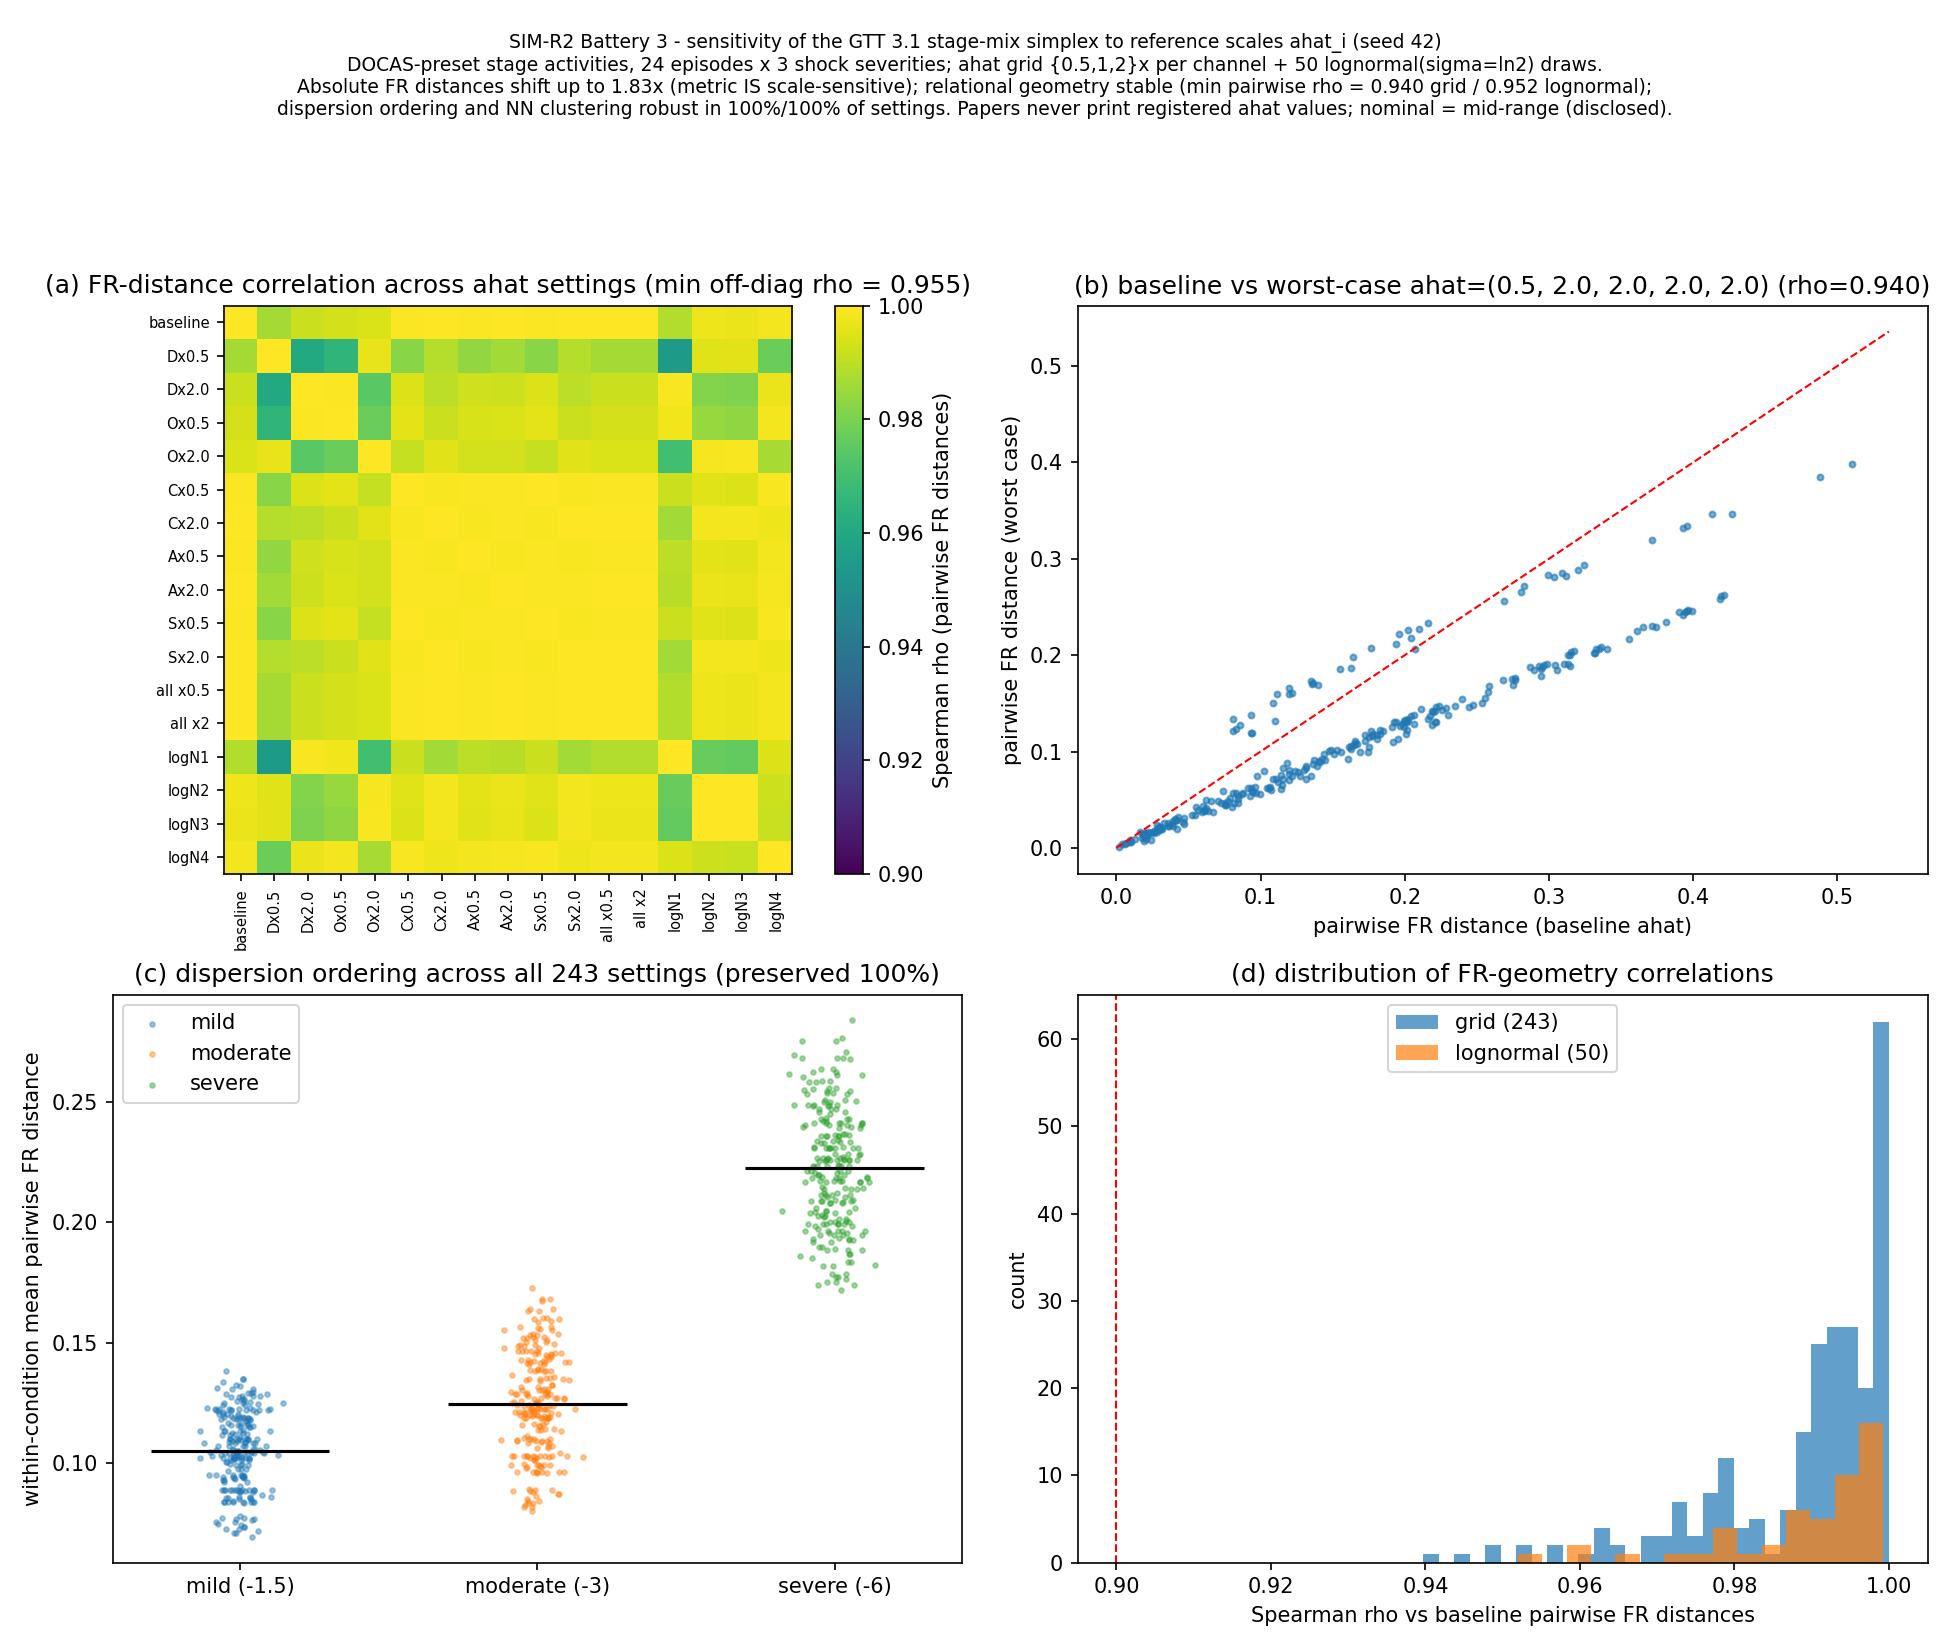
\includegraphics[width=\columnwidth]{figures/figR2_B3_fr_ahat_heatmap.png}
\caption*{\textbf{Figure SR1.} SIM-R2 battery 3 ($\hat{a}_i$ sensitivity of the \S 3.1 Fisher--Rao simplex): (a) 21-setting Spearman-$\rho$ heatmap of pairwise FR distances against the baseline; (b) baseline versus worst-case pairwise distances; (c) per-condition dispersion across all 243 grid settings --- the mild < moderate < severe ordering never inverts; (d) $\rho$ distributions (grid and log-normal perturbations).}
\end{figure}

\subsection*{3.2 Lyapunov stability of the alignment manifold [STANDARD]}

Write the continuous-time form of~\eqref{eq:stability} together with the relaxation of mismatch under corrective action:

\begin{equation}
dS/dt = \lambda \varepsilon, \quad d\varepsilon/dt = -\mu \varepsilon + \xi(t), \quad \mu > 0
\label{eq:flow}
\end{equation}

where the second equation expresses that activation (A) and environmental feedback dissipate mismatch at rate $\mu,$ with $\xi(t)$ exogenous forcing.

\begin{gttplain}[{Proposition 2}]

For $\xi = 0,$ the set $\{(\varepsilon, S) : \varepsilon = 0\}$ is a line of fixed points, globally attracting: $\varepsilon(t) \to 0$ exponentially at rate $\mu,$ and $S(t)$ converges to a finite limit.

\end{gttplain}

\begin{proof}[Derivation]

On the reduced dynamics $\dot{\varepsilon} = -\mu \varepsilon,$ the candidate Lyapunov function $L(\varepsilon) = \tfrac{1}{2} \varepsilon^{2}$ gives $\dot{L} = \varepsilon(-\mu \varepsilon) = -\mu \varepsilon^{2} \leq 0,$ with equality iff $\varepsilon = 0.$ Hence $\varepsilon = 0$ is globally asymptotically stable for the mismatch coordinate by Lyapunov's second method, and $S(t) = S_{0} + \lambda\int_{0}^{t} \varepsilon(s)$ ds converges to the finite limit

\end{proof}

\begin{equation}
S\infty = S_{0} + (\lambda/\mu)\varepsilon_{0}.
\label{eq:slimit}
\end{equation}

The Jacobian of the flow F(S, $\varepsilon$) = $(\lambda \varepsilon, -\mu \varepsilon)$ has eigenvalues $\{0, -\mu \}:$ the zero eigenvalue is the alignment line itself (each S is an equilibrium once $\varepsilon = 0),$ and the transverse eigenvalue $-\mu$ is the contraction rate of Definition 3. This is the standard stability statement for a linear dissipative system; it is derived here for self-containment.

\textbf{Discrete--continuous $\lambda$ convention.} The discrete per-event $\lambda$ (dimensionless, stable for $0 < \lambda < 1$) and the continuous-time $\lambda$ in $dS/dt = \lambda\varepsilon$ (units 1/time) are related by the event cadence; $S\infty = S_{0} + (\lambda/\mu)\varepsilon_{0}$ uses the continuous form. Estimation in \S{}6 uses the discrete form with the cadence caveat stated.

\textbf{Interpretation.} Alignment $E = V$ is the attractor; the total stability displacement from a perturbation $\varepsilon_{0}$ is $(\lambda/\mu)\varepsilon_{0}$ --- a gain under confirmation $(\varepsilon_{0} > 0),$ a cost under mismatch $(\varepsilon_{0} < 0)$ --- proportional to trust-sensitivity and inversely proportional to the system's corrective bandwidth. High-$\lambda$ systems (vigilant, threat-sensitive) move more stability per unit mismatch; high-$\mu$ systems (fast, honest feedback) move less. This is the formal core of the theory's design claim: immediate, verifiable feedback raises $\mu$ and thereby lowers the cost of trust maintenance.

\textbf{Long-run behavior: two pathologies and their repair [SIMULATION --- Sim G7].} The leak-free law~\eqref{eq:stability} is a pure integrator, and Proposition 2's displacement formula already signals the consequences. Sim G7 (long-horizon simulation, $10^{5}$ events, disclosed parameters $\lambda^{+} = 0.005, \lambda^{-} = 0.02, \delta =$ 0.01/event, $S_{base} = 0.5;$ \S{}3.6) confirms both horns: (i) under a stationary honest stream with small positive drift, $S$ grows \textbf{without bound} (S = 249 after $10^{5}$ events), so cross-agent comparability of $S$ is lost over long horizons; and (ii) a betrayal shock leaves a \textbf{permanent} displacement --- after a single $\varepsilon = -5$ shock followed by silence, $S$ remains displaced indefinitely (simulated: S = 10.4 forever), as the formula $S\infty = S_{0} + (\lambda/\mu)\varepsilon_{0}$ dictates. The biological preset of the master law (recognition gating $r_t$ and a baseline-restoring leak $\delta_S > 0$ toward a homeostatic prior $S_{base},$ not toward zero) repairs both: after the same shock, $S$ recovers to within 10\% of $S_{base}$ in 69 events (138 and 207 events for the -10 and -20 shocks, matching the closed form at every shock size), exponentially at the rate set by $\delta_S,$ with small betrayals $(\lambda^{-}|\varepsilon| \lesssim 0.05,$ i.e. $|\varepsilon| \lesssim 2.5$ at these parameters) absorbed without measurable displacement --- an honest null: the \emph{reconciled} law does not scar permanently from small events, and the leak-free law's ``permanent scar'' is a pathology of the pure integrator, not a feature to celebrate. (A leak toward zero instead of toward a baseline produces the opposite pathology --- trust decaying to indistinguishability-from-absence without events, with a simulated half-life of 69 events at $\delta = 0.01$ --- which is precisely why the biological layer's leak is baseline-restoring; see the companion preprint, \S{}2.9.) The physics layer's leak-free form is retained because it is the tractable limit in which the geometry and statistics of \S{}3.1 -- 3.4 are derivable in closed form; the biological layer is the intended model of organisms.

\subsection*{3.3 Stochastic extension: Langevin and Fokker -- Planck dynamics [STANDARD], with observation-dependent dissipation [DERIVED]}

Real feedback is noisy. Model mismatch as an Ornstein -- Uhlenbeck process:

\begin{equation}
d\varepsilon = -\mu \varepsilon dt + \sigma dW_t
\label{eq:ou}
\end{equation}

with innovation intensity $\sigma$ (units: $\sigma^{2}$ in 1/time after Definition 2a normalization, so $\mathrm{Var}_{stat}$ below is dimensionless). The associated Fokker -- Planck equation for the density $p(\varepsilon, t)$ is

\begin{equation}
\partial p/\partial t = \mu \partial(\varepsilon p)/\partial \varepsilon + (\sigma^{2}/2) \partial^{2}p/\partial \varepsilon^{2}
\label{eq:fp}
\end{equation}

whose stationary solution is Gaussian:

\begin{equation}
\begin{split}
p_{stat}(\varepsilon) &= \sqrt{\mu/\pi \sigma^{2}} \exp(-\mu \varepsilon^{2}/\sigma^{2})\\
&\qquad \mathrm{Var}_{stat}(\varepsilon) = \sigma^{2}/2\mu.
\end{split}
\label{eq:stationary}
\end{equation}

\textbf{Interpretation.} Even a well-functioning trust system fluctuates around alignment with stationary variance $\sigma^{2}/2\mu:$ residual prediction error is the operating cost of functioning in a stochastic environment. This stationary variance --- small for tight alignment maintenance, large for noisy, poorly corrected alignment --- is the theory's precise, derived replacement for any ``order versus chaos'' dichotomy (\S{}1.3): neither pole is a bifurcation, and no critical point exists in the single-agent dynamics.

\textbf{Observation-dependent dissipation [DERIVED from \eqref{eq:ou}].} The act of measurement enters the dynamics as a modulation of the dissipation rate. Let $m_t \geq 0$ be the \textbf{measurement-salience} of the observation regime at time $t$ --- a dimensionless scalar increasing in (i) the subject's awareness of being measured, (ii) the audience and persistence of the measurement record, and (iii) the stakes attached to it; $m_t = 0$ for measurement that is local, consent-bearing, ephemeral, and accountable. $m$ is a property of the observation channel, not of the trust state. Let the \textbf{observation-dissipation coefficient} $\psi : \mathbb{R}\geq0 \to \mathbb{R}$ be $C^{1},$ with units of 1/time (the units of $\mu),$ satisfying $\psi(0) = 0$ (non-salient observation reduces to the unperturbed OU process) and $\psi(m) \geq -\mu$ for all $m$ (total dissipation stays non-negative --- no anti-damping). The sign of $\psi$ encodes direction: $\psi > 0$ is the habituation regime (sustained salient observation \emph{raises} dissipation); $\psi < 0$ is the hypervigilance/chilling regime (salient observation \emph{lowers} dissipation). The mismatch process becomes

\begin{equation}
d\varepsilon = -(\mu + \psi(m_t)) \varepsilon dt + \sigma dW_t, \quad \dot{S} = \lambda \varepsilon,
\label{eq:oupsi}
\end{equation}

i.e., Eq.~\eqref{eq:ou} with a slowly modulated drift coefficient --- standard, simulable, and estimable. (No continuum field equation on $\mathbb{R}^{5}$ is defined or needed: the theory's dynamics live on the $(S, \varepsilon)$ state space, and measurement dependence is fully expressed through the scalar coefficient $\psi.$)

\textbf{Derived observable consequences} (from \eqref{eq:stationary}, exact for constant m):

\begin{itemize}

\item \textbf{Stationary variance:} $\mathrm{Var}_{stat}(\varepsilon) = \sigma^{2} / (2(\mu + \psi(m))).$

\item \textbf{Autocorrelation time:} $\tau_c = 1 / (\mu + \psi(m)).$

\item \textbf{Critical slowing as $\psi \to -\mu^{+}:$} variance and autocorrelation time both diverge $\propto (\mu + \psi)^{-1}.$ Hypervigilant regimes are therefore identifiable by \emph{rising variance jointly with rising lag-1 autocorrelation} of the mismatch stream --- the standard early-warning statistic, and the falsifiable form of this paper's H4 (\S{}6) and of the chilling-effects argument of the companion protocol preprint.

\end{itemize}

\textbf{Numerical verification [SIMULATION --- Sim G9].} Exact OU discretization (64 chains $\times 10^{5}$ -- $3\cdot10^{5}$ steps, $\geq 30$ autocorrelation times per run, seed 42, $\mu = \sigma = 1$) reproduces both derived quantities across $\psi/\mu \in$ [-0.95, +1.00]: simulated/theory stationary-variance ratio $\in [0.992, 1.004];$ lag-1 autocorrelation matches $e^(-(\mu+\psi))$ within $\pm0.006.$ The distortion inflation factors relative to the unobserved baseline are: \textbf{$\psi = -0.2\mu \to \times1.25;$ $\psi = -0.5\mu \to \times2.0;$ $\psi = -0.9\mu \to \times10$} in both variance and memory. The habituation branch is verified as well $(\psi = +\mu:$ Var 0.250 simulated vs 0.250 theory).

\textbf{The honesty condition: $\psi = 0$ is not achievable by any architecture, including ours.} $\psi \to 0$ requires $m \to 0;$ the four architectural responses of the companion protocol (local-first storage, consent-bearing queries, accountable access logs, minimized disclosure) drive salience toward $m_{\min}$ --- but $m_{\min} > 0,$ hence $\psi \to \psi(m_{\min}) < 0,$ not 0. \textbf{TFP's own measurement still distorts:} at an illustrative residual salience $\psi = -0.05\mu,$ mismatch variance and memory remain inflated by $\times1.05$ (Sim G9). The architecture minimizes observation-driven distortion; it does not eliminate it, and GTT's own axiom --- observation is never neutral --- applies to the stack's own instruments. No claim of $\psi = 0$ is made anywhere in this stack.

\subsection*{3.4 Collective dynamics: the Kuramoto analogy and the Phase Alignment Score [ANALOGY]}

Consider $N$ agents (or N institutional nodes) each carrying a phase $\theta_k$ representing the alignment state of its expectation -- validation loop, coupled through shared feedback channels:

\begin{equation}
d\theta_k/dt = \omega_k + (K/N) \Sigma_j \sin(\theta_j - \theta_k)
\label{eq:kuramoto}
\end{equation}

This is the Kuramoto model (Kuramoto, 1984). Define the order parameter

\begin{equation}
R e^{i\psi_K} = (1/N) \Sigma_k e^{i\theta_k}
\label{eq:order}
\end{equation}

(The phase of the mean field is written $\psi_K$ here to distinguish it from the dissipation coefficient $\psi$ of \S{}3.3.) $R \in [0, 1]$ measures collective phase alignment. For a unimodal symmetric frequency distribution $g(\omega),$ the incoherent state $R = 0$ loses stability at the critical coupling

\begin{equation}
K_c = 2 / (\pi g(0))
\label{eq:kc}
\end{equation}

above which a phase-locked solution with $R \sim \sqrt{1 - K_c/K}$ emerges continuously (Strogatz, 2000).

\begin{gttdef}[{Definition 4 (Phase Alignment Score)}]

PAS is the empirical order parameter of a trust network: PAS = $R$ computed over the alignment phases of interacting nodes, with phase assigned from each node's \emph{normalized} residual mismatch by the \textbf{stereographic map}

\end{gttdef}

\begin{equation}
\begin{split}
\theta_k &= 2 \arctan(\tilde{\varepsilon}_k) \in (-\pi, \pi]\\
&\qquad \tilde{\varepsilon}_k = (V_k - E_k)/s_k \quad \text{(dimensionless, Def.~2a),}
\end{split}
\label{eq:pasmap}
\end{equation}

covering the full circle, with $\theta = 0$ at perfect alignment and $\theta \to \pm \pi$ as mismatch saturates --- ``maximally betrayed'' and ``maximally over-validated'' meet at the antipode, the correct topology for a circular alignment variable. Two verified properties give PAS a principled null model: (i) if $\tilde{\varepsilon} \sim$ Cauchy(0, 1) --- heavy-tailed, matching the stack's own event-outcome stylized fact --- then $\theta$ is \emph{uniform} on $(-\pi, \pi)$ (the stereographic projection of the Cauchy law), so an unaligned population has $R \approx 1/\sqrt{N}$ at zero coupling, the incoherent baseline the Kuramoto analysis requires (in silico: R = 0.026 at N = 2000, finite-size floor $1/\sqrt{N} = 0.022);$ (ii) for $\tilde{\varepsilon} \sim$ Cauchy(0, s'), $\theta$ is wrapped-Cauchy with mean resultant length $\rho$ = |1 - s'|/(1 + s'), interpolating smoothly between concentrated-at-zero (aligned population) and uniform --- population alignment maps onto the standard wrapped-Cauchy concentration parameter.

\textbf{Phase-map choice: stereographic, not arctan.} The half-circle assignment $\theta_k \propto \arctan(\varepsilon_k)$ occupies only half the circle and biases $R$ upward even at zero coupling: with Cauchy-distributed mismatches that map reports $R \approx 0.63$ at $K = 0$ --- an ``incoherent control'' showing strong coherence (Technical Appendix, Sim-Battery B, control battery: 0.635 $\pm$ 0.014 over 200 seeds, N = 500; the Technical Appendix --- the stack's simulation batteries and mathematical development --- is bundled with the Supporting Document (deposit pending) and is cited below as ``Technical Appendix, Sim-Battery A/B, Study N'' or ``Technical Appendix, \S{}M''). The stereographic map of Definition 4 gives 0.040 $\pm$ 0.021 at $K = 0,$ at the finite-size floor $(1/\sqrt{500} \approx 0.045),$ matching raw uniform phases $(0.039 \pm 0.020)$ --- and matching the isolated control $R = 0.032$ reported in the companion protocol's Sim P1 run. The control baseline for all coherence claims in this stack is therefore $\approx 0.03$--$0.05,$ not 0.63.

\begin{figure}[!tb]
\centering
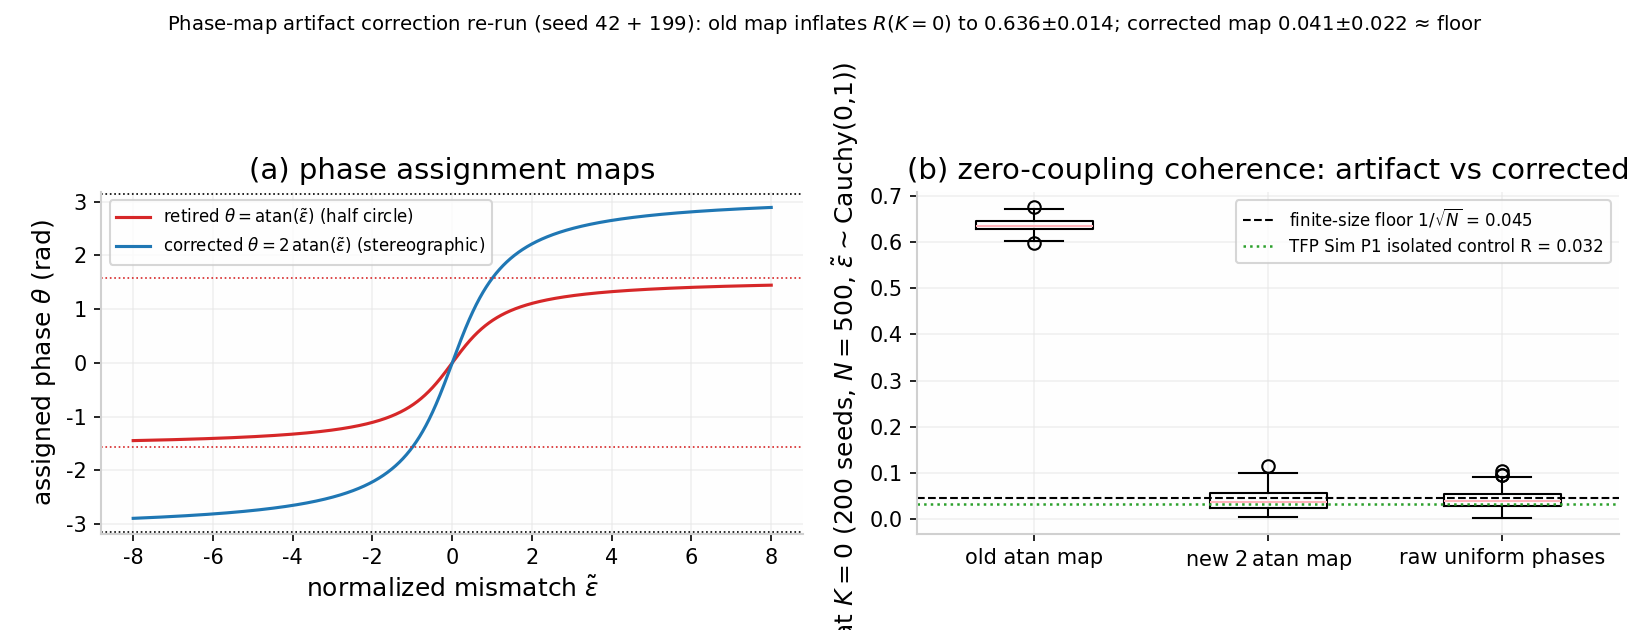
\includegraphics[width=\columnwidth]{figures/fig_phasemap_control.png}
\caption*{\textbf{Figure S1.} Phase-map control battery (200 seeds, $K = 0$, $N = 500$, Cauchy$(0,1)$ mismatches; \S 3.4). (a) The half-circle arctan map occupies only half the circle; the stereographic map $\theta = 2\arctan(\tilde{\varepsilon})$ covers it. (b) Zero-coupling coherence: the half-circle map reports $R = 0.636 \pm 0.014$ (artifact); the stereographic map restores the finite-size floor at $0.041 \pm 0.022$, matching raw uniform phases ($0.042 \pm 0.021$) and the TFP Sim P1 isolated control ($R = 0.032$).}
\end{figure}

\textbf{Status of $K_c:$ mean-field reference, not prediction.} Equation~\eqref{eq:kc} is valid under all-to-all coupling, $N \to \infty,$ a time-stationary unimodal symmetric $g(\omega),$ and full-circle phases. On sparse weighted trust networks the true threshold will differ by network corrections (\S{}7, limitations). Accordingly, \eqref{eq:kc} supplies the \emph{functional form} of the hypothesis --- a continuous onset of PAS coherence at a critical feedback quality --- not a numerical prediction of where the threshold lies.

\textbf{Sparse-network sensitivity --- run, not deferred (SIM-R2 battery 4; [SIMULATION]).} The network corrections flagged above are now measured. The Sim $G1(b)$ protocol ($N = 500,$ unit-Cauchy natural frequencies, stereographic initialization, degree-normalized coupling $K/k_i$ so $K$ is comparable across topologies) re-run on Erd\H{o}s -- R\'enyi ($p \in \{0.05, 0.1, 0.2, 0.5\};$ $\langle k\rangle \approx 25/49/100/249$), Barab\'asi -- Albert ($m = 12$ and $m = 2;$ $\langle k\rangle \approx 24$ and 4), and log-normal-weighted all-to-all graphs reproduces the published operating point exactly (all-to-all $R(K = 4.5) = 0.710 \pm 0.029$ vs.\ Sim G1's 0.709; TFP's Sim P1 verification re-run reports $0.739 \pm 0.029$ at the same nominal operating point --- P1's ABM-with-adversaries protocol and P1c's/G1's pure-Kuramoto protocol differ, and the $\sim$0.03 gap is within seed noise) and shows that \textbf{$R > 0.7$ at $K = 4.5$ fails under sparsity}: ER $p = 0.05 \to 0.684;$ BA $m = 12 \to 0.687$ (both below target, within $\sim$1 sd); BA $m = 2 \to 0.416,$ never recovering above 0.7 even at $K = 8.$ ER $p \geq 0.2$ and the log-normal-weighted all-to-all pass: the threat is \emph{missing edges} (mean degree $\langle k\rangle \lesssim 25$), not heterogeneous weights. The functional form survives everywhere --- every topology shows the same continuous onset at $K_c \approx 2$ (the mean-field $K_c = 2$ for Cauchy$(0,1)$ survives degree normalization); what shifts is the asymptote level and the margin above threshold. The functional-form-only posture adopted above is therefore confirmed as necessary and, on the tested topology family, sufficient; the defensible population claim needs $K \geq 6$ -- $8$ \emph{and} $\langle k\rangle \gtrsim 25$ (Figure SR2).

\begin{figure}[!tb]
\centering
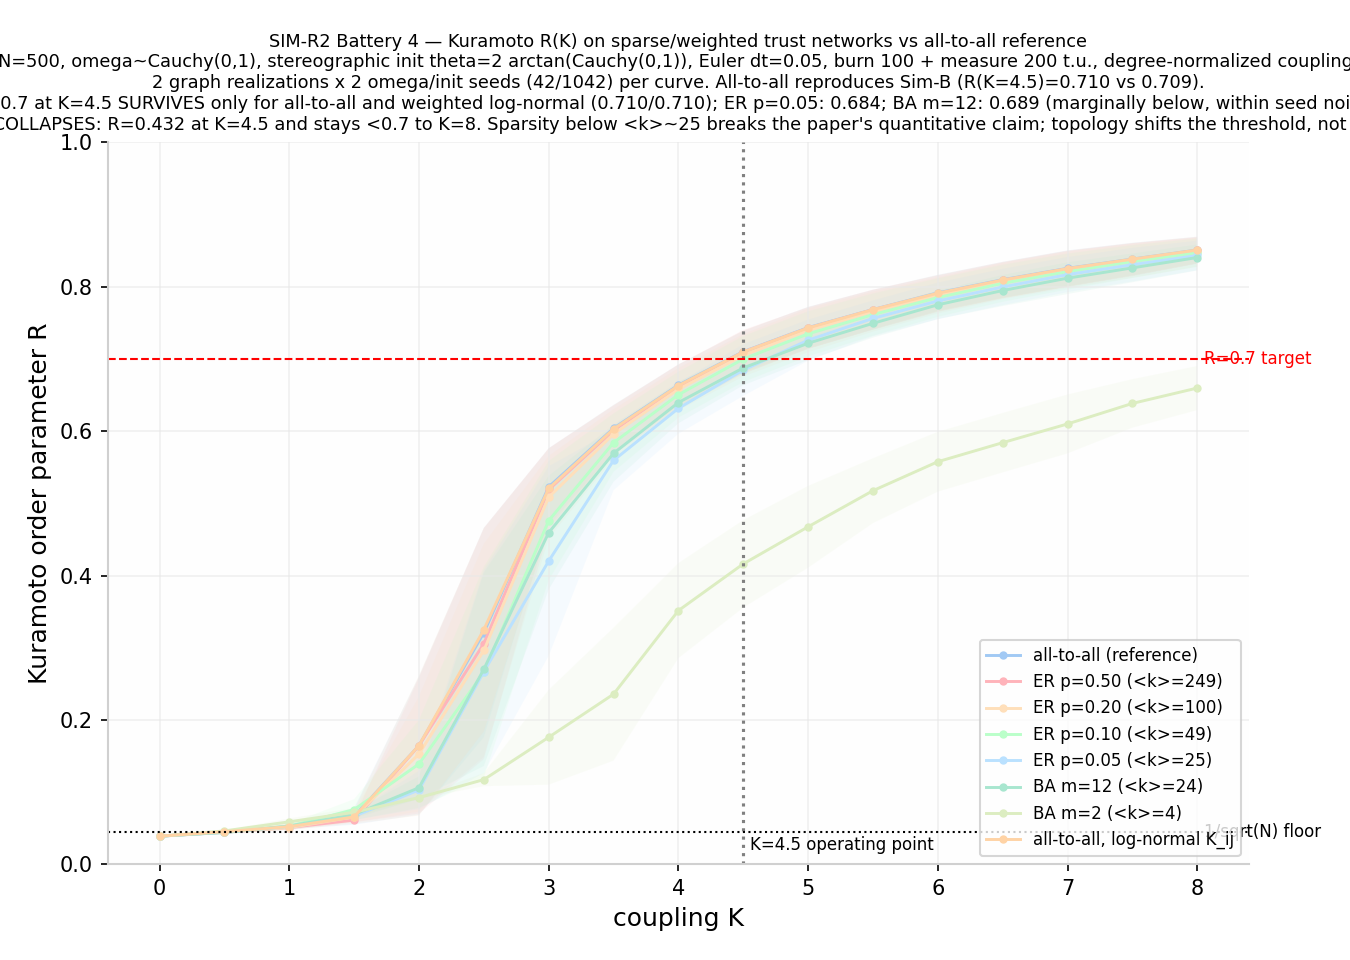
\includegraphics[width=\columnwidth]{figures/figR2_B4_kuramoto_topologies.png}
\caption*{\textbf{Figure SR2.} SIM-R2 battery 4: Kuramoto $R(K)$ per topology (mean $\pm$ sd over 2 graph realizations $\times$ 2 seeds) against the all-to-all reference, with the $R = 0.7$ target, the $1/\sqrt{N}$ floor, and the $K = 4.5$ operating point marked. The onset $K_c \approx 2$ is topology-invariant; the $K = 4.5$ coherence level is not (\S 3.4).}
\end{figure}

\textbf{Interpretation and status.} The mapping is: expectation -- validation alignment $\leftrightarrow$ oscillator phase; feedback bandwidth and $latency^{-1} \leftrightarrow$ coupling $K;$ systemic trust $\leftrightarrow R.$ The falsifiable content (developed as H3, \S{}6) is that trust networks exhibit a threshold in feedback quality below which collective trust cannot self-sustain regardless of individual dispositions. This is asserted as a formal analogy: no claim is made that trust oscillators are physical oscillators; the claim is that the bifurcation structure of \eqref{eq:kuramoto}--\eqref{eq:kc} is the appropriate functional form for collective trust transitions, testable against network data. The import is functional-form-only: no natural frequency $\omega$ is identified in trust terms --- the $\omega_k$ of \eqref{eq:kuramoto} have no measured counterpart, and that is the analogy's known limit.

\subsection*{3.5 Measurement: four senses, disambiguated}

The phrase ``trust is always a measurement'' carries several distinct meanings. They are separated here into four distinct, numbered claims, each with its own label and evidential basis. No single one borrows authority from another.

\textbf{Sense 1 --- Statistical estimation [STANDARD/DERIVED].} The trust state is estimated from finite data, with quantifiable precision limits: the Cramér -- Rao bound on $\Delta^{4}$ (\S{}3.1) and the stationary statistics of the mismatch stream (\S{}3.3). This is the primary, load-bearing sense: trust is something \emph{measured}, with error bars, not a disembodied property.

\textbf{Sense 2 --- Frame-dependence (a controlled metaphor).} The law~\eqref{eq:stability} is asserted form-invariant across observers while its parameters $(\lambda, \mu)$ are observer-specific (\S{}2.4). The parallel to relativity is a metaphor for parameter-observer relativity; no transformation law or invariant is claimed. Its empirical content is the invariance hypothesis H2a (\S{}6), which can fail.

\textbf{Sense 3 --- Social observation effects [DERIVED + EMPIRICAL].} Observation changes the dynamics being observed, through the observation-dissipation coefficient $\psi(m)$ of \S{}3.3: salient measurement lengthens mismatch memory and inflates its stationary variance (dissipation-floor slowing as $\psi \to -\mu^{+}),$ with the chilling-effects literature demonstrating the phenomenon at population scale (Penney, 2016; \S{}6 H4). This sense is a quantitative claim about the $(S, \varepsilon)$ dynamics, verified in silico (Sim G9) and falsifiable in the field.

\textbf{Sense 4 --- Quantum decoherence homology [HOMOLOGY --- zero inferential load].} In quantum measurement, environmental entanglement selects preferred (``pointer'') states and suppresses off-diagonal coherence --- environment-induced superselection (Zurek, 2003). GTT's measurement structure is \emph{homologous in form}:

\begin{table}[!tb]
\centering\footnotesize
\caption*{\textbf{Table 1.} The quantum-decoherence correspondence of \S 3.5 (Sense 4): a labeled structural homology carrying zero inferential load.}
\begin{tabular}{@{}>{\raggedright\arraybackslash}p{0.46\columnwidth}>{\raggedright\arraybackslash}p{0.48\columnwidth}@{}}
\toprule
\textbf{Quantum measurement} & \textbf{GTT trust measurement} \\
\midrule
Superposition of outcome amplitudes & Expectation $E$ as a distribution over anticipated outcomes \\
\addlinespace[2pt]
Environmental entanglement / monitoring & Validation channel $V$ returning environmental feedback \\
\addlinespace[2pt]
Decoherence $\to$ pointer-state selection & Recognition $(C):$ mismatch detection resolves the distribution onto an outcome \\
\addlinespace[2pt]
Post-measurement eigenstate & Stabilization $S:$ updated baseline becomes the next prior \\
\addlinespace[2pt]
Measurement changes the system measured & Observation changes trust dynamics $(\psi,$ \S{}3.3; chilling effects, Sense 3) \\
\addlinespace[2pt]
\bottomrule
\end{tabular}
\end{table}

The right-hand column is classical stochastic dynamics; \textbf{nothing quantum-mechanical is claimed for brains, markets, or any social system.} The homology is asserted at the level of measurement structure --- the role of environmental coupling in converting an unresolved predictive distribution into a definite registered state --- in the same spirit that \S{}2.4's frame correspondence is asserted at the level of parameter structure. It carries \textbf{zero inferential load}: no GTT result is derived from it, no quantum evidence is offered for any social claim, and deleting this subsection would change no prediction of the theory.

\emph{On the physics once invoked here, stated plainly.} Leggett -- Garg inequalities --- temporal analogs of Bell inequalities testing macrorealism and noninvasive measurability (Leggett \& Garg, 1985) --- have been violated in superconducting flux qubits well above the single-atom scale (Palacios-Laloy et al., 2010). That is a fact about macroscopic \emph{quantum} systems; the category gap between qubit macrorealism and sociological observation is not bridgeable by citation, and this paper does not treat those experiments as evidence for anything in the social column --- they are mentioned only to document that ``measurement back-action in coupled systems'' is a coherent physical concept, the weakest possible use. The biological leg once offered for quantum-adjacent effects --- wavelike energy transfer in photosynthetic complexes (Engel et al., 2007) --- is undercut on its own terms: Cao et al. (2020) conclude that interexciton coherences are too short-lived to bear the functional significance originally proposed, relocating the relevant quantum effects to vibronic coupling and tunneling. GTT accordingly makes no biological-quantum claim of any kind; the homology above stands on its structural statement alone or not at all.

\textbf{The social-scale signature, restated in the theory's own terms.} The operational consequence at the scale where GTT lives needs no quantum vocabulary: leakage of measurement information raises observation salience $m,$ and through $\psi$ (\S{}3.3) changes the dynamics being observed. Privacy erosion functions as uncontrolled measurement --- a continuous performance condition undermining the freedom necessary for error, reflection, and learning (Warren \& Brandeis, 1890; Solove, 2008). Surveillance-driven chilling (Penney, 2016) and algorithmic amplification of fear and outrage for engagement (Tufekci, 2015; O'Neil, 2016) are the measurable high-salience channels of networked trust systems. The design consequence --- measurement must be local, consent-bearing, and accountable (driving m, hence $|\psi|,$ toward its floor; never to zero, \S{}3.3) --- is carried into the companion protocol as an engineering constraint.

\subsection*{3.6 Numerical verification of the dynamics [SIMULATION]}

The analytical claims of \S{}3.1 -- 3.4 were verified numerically against pre-registered criteria (criteria specified in code before the reported runs; full protocols, seeds, and audit trails in the Supporting Document, \S{}L and \S{}S). \textbf{Disclosure of planted values:} every parameter appearing in these simulations --- $\lambda = 0.35$ (Sims G1, G6, and the companion preprint's operator-recovery check, recovered slope 0.348, $R^{2} = 0.970),$ the regression slope 0.174 reported in the companion preprint, \S{}5.5 (an eligibility-rescaled estimator check, not a $\lambda$ estimate), and $\lambda = 0.02$ (the TFP threshold study, Sim P8) --- is a \textbf{simulation parameter or recovery check, not a prediction or estimate of any population quantity}. The only prospective empirical claim about $\lambda's$ value is \S{}6 H2.

\textbf{Interpretation note.} Sims G1 and G6 sample initial conditions on $\Delta^{4}$ directly; following \S{}3.1, those trajectories are interpreted as stage-mix profiles $\theta(t),$ with the stability law acting on the underlying $(S, \varepsilon)$ and $\theta$ a derived readout. Stated explicitly: the trajectory object is $(S(t), \varepsilon(t))$; the on-simplex readout $\theta(t)$ is a derived map from channel activities to the stage-mix profile (normalized non-negative stage activities, \S{}3.1), evaluated post hoc on the dynamics --- no separate on-simplex dynamics is asserted; the Fisher--Rao convergence figures visualize the readout, not an independent flow. Because Sims G1 and G6 sample $\theta$ directly, no $\hat{a}$ enters; \S{}3.1 rule (i) is vacuous for their absolute distances.

\textbf{Sim G1} --- three pre-registered checks:

\begin{itemize}

\item \textbf{(a) Fixed-point stability [SUPPORTED].} 200 random initial conditions on $\Delta^{4}$ under the discrete stability law $(\lambda = 0.35$ --- planted, matched expectation/validation): all trajectories converge to the alignment fixed point $T^{*}$ (final Fisher -- Rao distance 0.0; median 10 steps to d < 0.01). The Lyapunov claim of \S{}3.2 holds computationally, not just analytically.

\item \textbf{(b) Synchronization bifurcation [SUPPORTED --- analogy structure only].} A Kuramoto population (N = 500, unit-Cauchy natural frequencies) shows $R < 0.3$ everywhere below the mean-field reference $K_c = 2$ (Eq.~\eqref{eq:kc}), a steep transition band (R rises 0.25 $\to 0.75$ over $K \in [2,$ 4.5]), and PAS-level coherence $(R > 0.7)$ by $K = 4.5$ (all-to-all; fails for $\langle k\rangle \lesssim 25$, \S{}3.4 SR2), reaching $R = 0.89$ at $K = 10.$ Finite-size scaling $(N = 500/2000/5000)$ confirms the $R = 0.7$ crossing is a property of the order-parameter curve, not a finite-N artifact. This verifies that the \emph{analogy's functional form} behaves as the mean-field analysis says --- it is not evidence about trust networks (see \S{}3.4, $K_c$ status).

\item \textbf{(c) Langevin robustness [SUPPORTED].} Under additive noise of intensity $\sigma$ (SDE convention, \S{}3.3), the stationary distribution concentrates near $T^{*}$ with a linear noise floor $(\bar{d} \approx 3.3\sigma$ over $\sigma \in [0.01,$ 0.5]); a destroyed fixed point would show $\bar{d} \approx 1.2$ -- 1.4 independent of $\sigma.$

\end{itemize}

\begin{figure}[!tb]
\centering
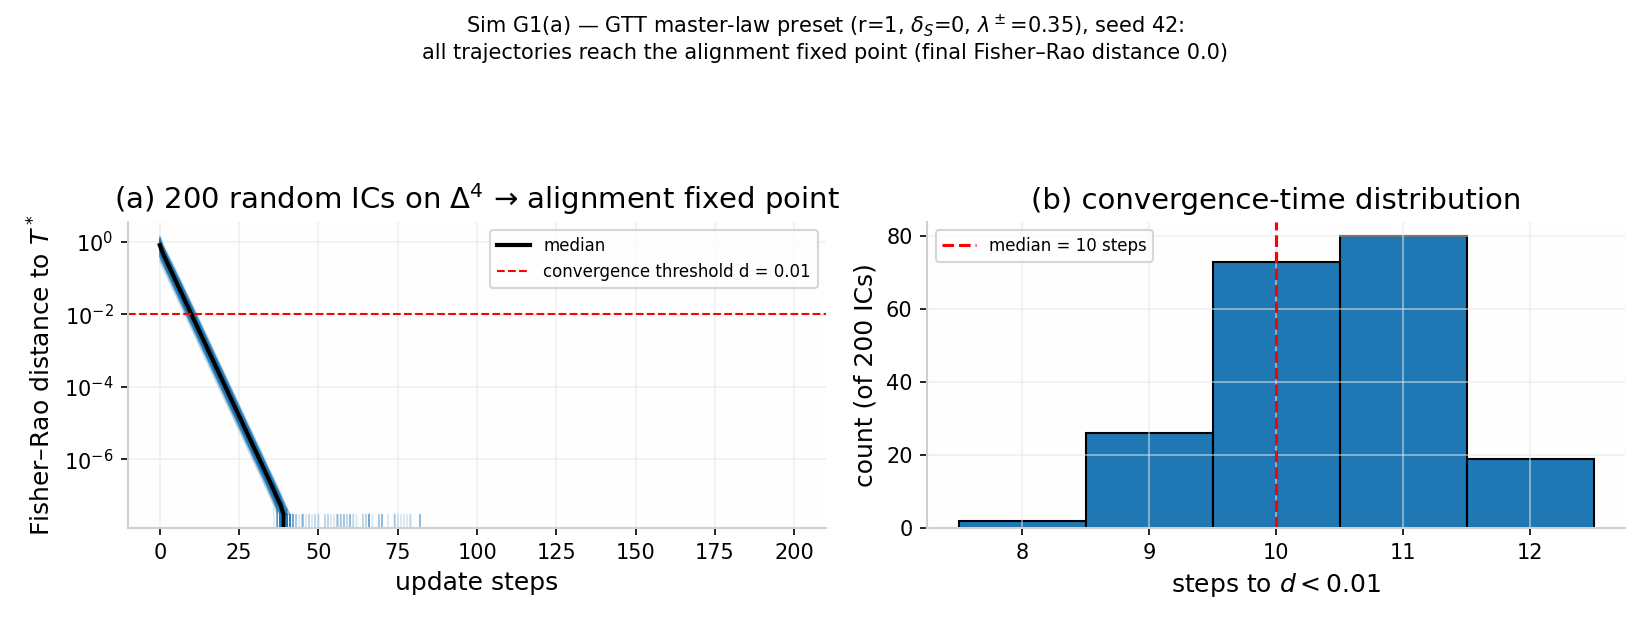
\includegraphics[width=\columnwidth]{figures/figG1_convergence.png}
\caption*{\textbf{Figure S2.} Sim G1(a): convergence to the alignment fixed point from 200 random initial conditions on $\Delta^{4}$ (planted $\lambda = 0.35$). Fisher--Rao distance trajectories and convergence-time histogram: final distance $0.0$ for all trajectories, median 10 steps to $d < 0.01$ (\S 3.6).}
\end{figure}

\begin{figure}[!tb]
\centering
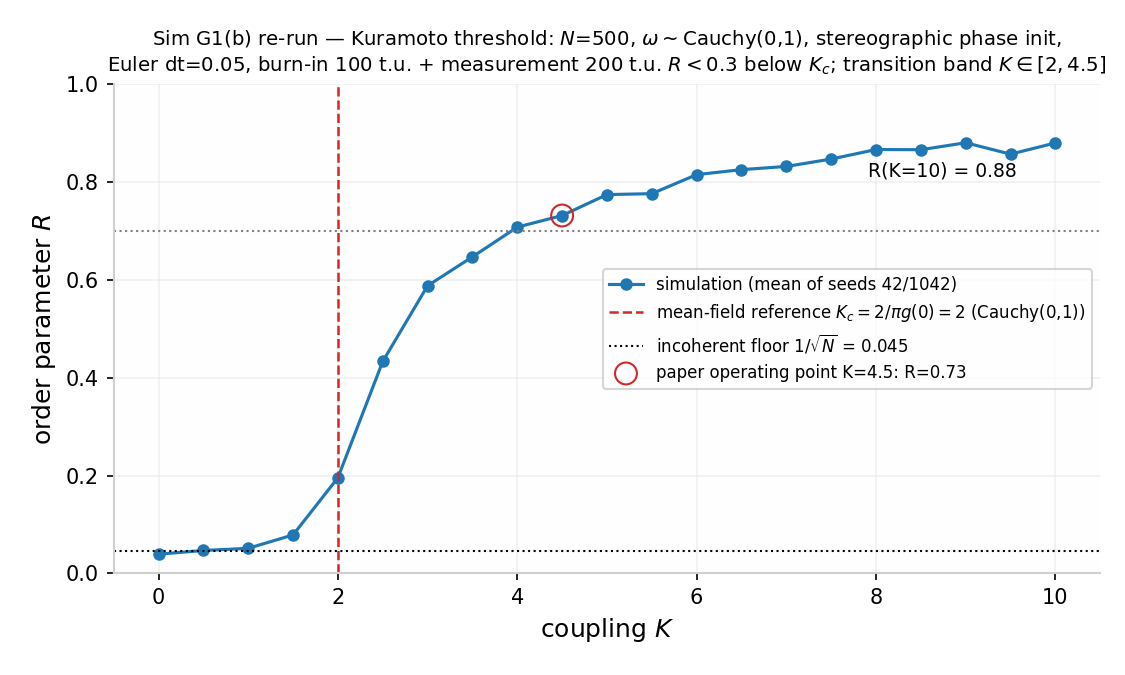
\includegraphics[width=\columnwidth]{figures/fig_kuramoto_threshold.png}
\caption*{\textbf{Figure S3.} Sim G1(b): Kuramoto order parameter $R$ versus coupling $K$ ($N = 500$, unit-Cauchy natural frequencies). Incoherent ($R < 0.3$) everywhere below the mean-field reference $K_c = 2$ (Eq.~\eqref{eq:kc}); finite-size floor $1/\sqrt{N}$; PAS-level coherence ($R > 0.7$) by $K \approx 4.5$. Analogy structure only (\S 3.4, \S 3.6).}
\end{figure}

\textbf{Sim G6} (seed 20260908; full audit trail in the Supporting Document, \S{}S) --- state-space geometry and temporal structure:

\begin{itemize}

\item \textbf{M1 --- Manifold contraction [SUPPORTED].} Sixty uniform-random initial conditions on $\Delta^{4}$ contract onto the single attractor: mean Hellinger-chord distance to $T^{*}$ falls from 0.295 to 0.016 (distance convention per the replication note below) (dispersion ratio 0.053, BCa bootstrap 95\% CI [0.0475, 0.0594]; worst case 0.031 < 0.05). The state space of the theory is a manifold with one attracting basin (Figure 4a -- b; re-implemented as Figure SR5) --- the computational counterpart of Definition 3's uniform contraction. The same qualifier M2 carries applies here: the contraction is by construction of the stated linear law --- this verifies the implementation, not the world. \textbf{Replication note.} An independent re-implementation of this specification (seed 20260908; 60 uniform-random initial conditions on $\Delta^{4}$; discrete law, $\lambda = 0.35$ planted; code and results JSON in the deposit) reproduces the qualitative result --- 60/60 trajectories inside the $d < 0.05$ band, mean distance 0.288 $\to$ 0.013 at step 7 --- while the dispersion ratio differs beyond bootstrap noise: 0.047 (95\% bootstrap CI [0.0447, 0.0473]) vs the printed 0.053 [0.0475, 0.0594], non-overlapping intervals, so bit-identity is not claimed. The re-implementation also shows the printed absolute distances to be on the $\sqrt{\theta}$-sphere \emph{chord} (Hellinger) convention: the Fisher -- Rao arc is a monotone reparameterization, and the dispersion ratio is near-identical under either. The printed values stand as the original run's record, pending bit-identity against the original battery (deposited separately).

\begin{figure}[!tb]
\centering
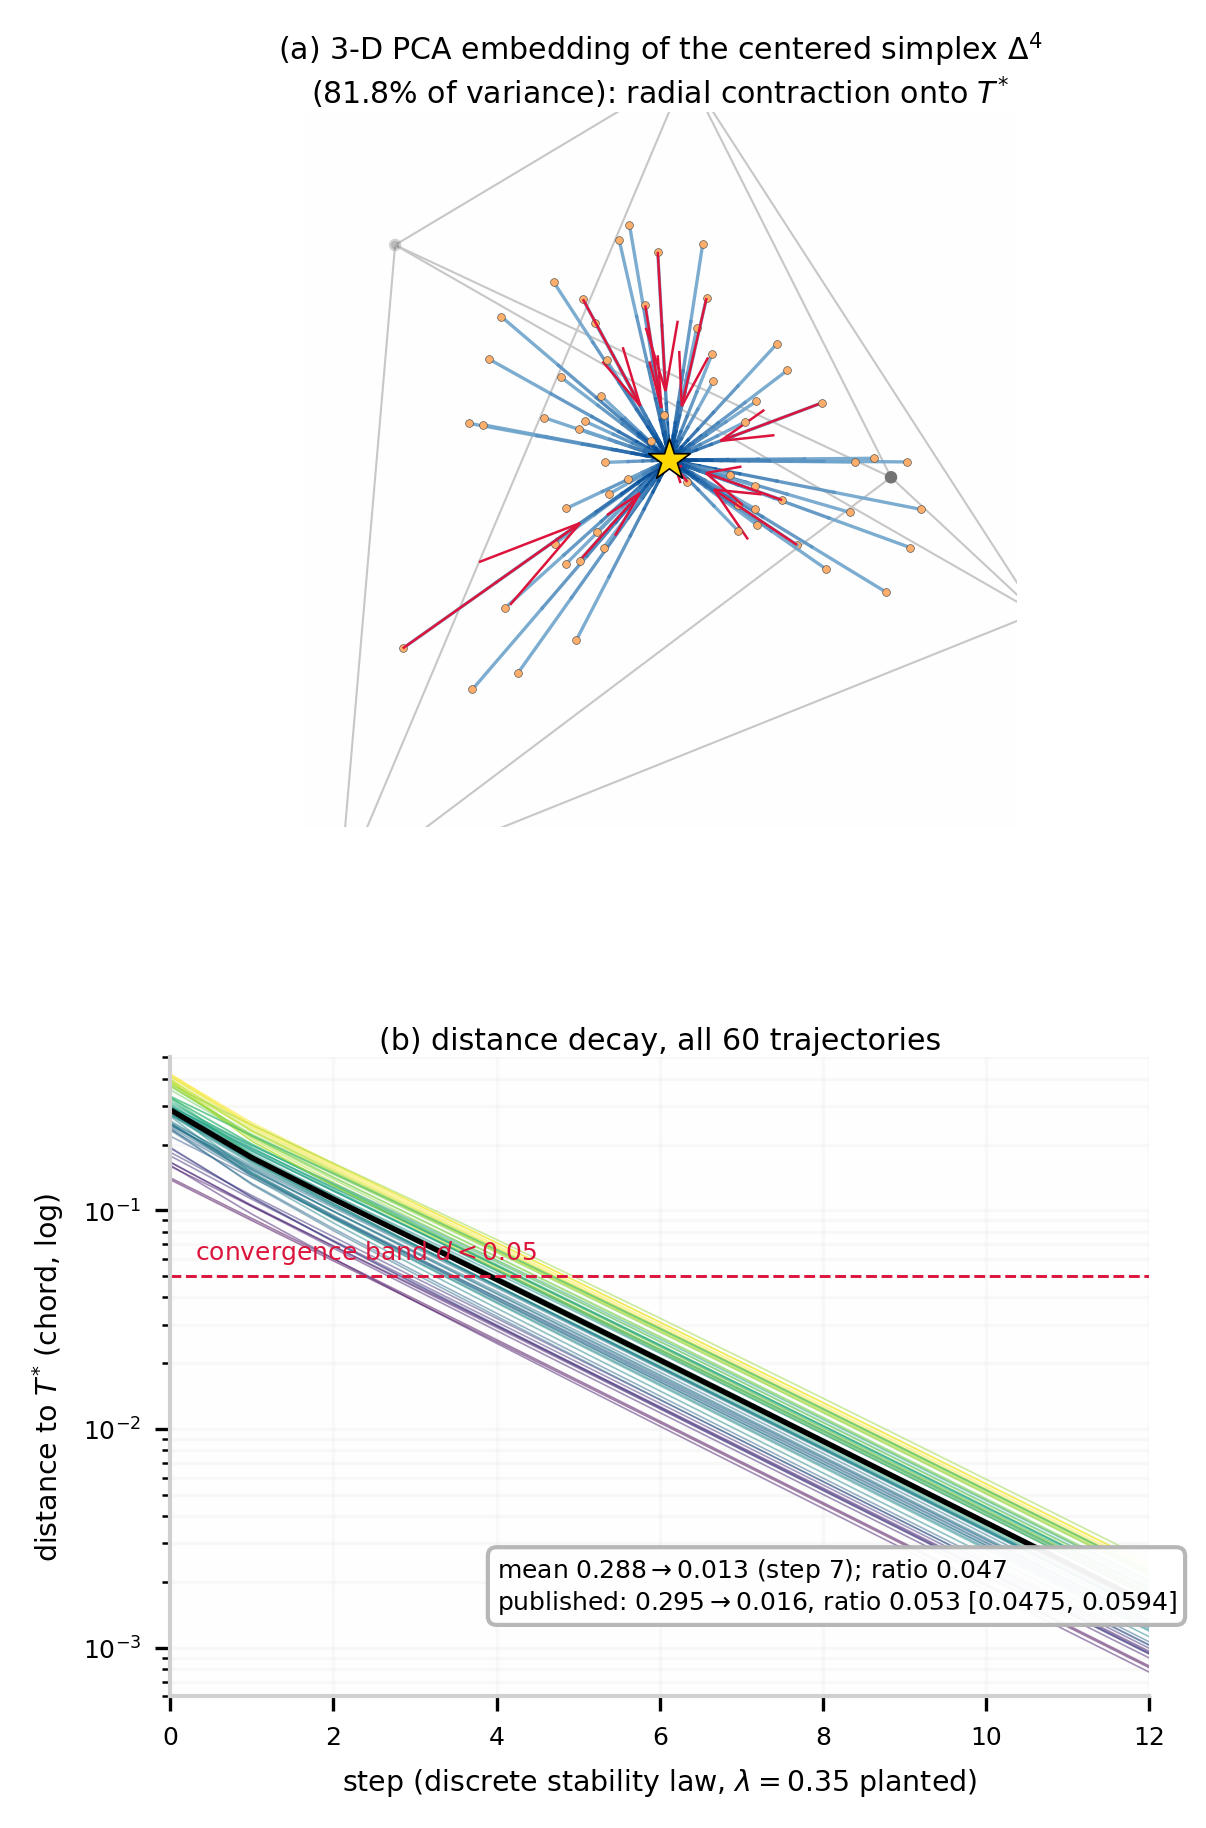
\includegraphics[width=\columnwidth]{figures/figG6_manifold_3d_column.png}
\caption*{\textbf{Figure SR5.} The trust manifold rendered (Sim G6-M1, independent re-implementation of the published specification; seed 20260908). (a) 3-D PCA embedding of the centered simplex $\Delta^{4}$ (81.8\% of trajectory variance): 60 stage-mix trajectories (light $\to$ dark with time; orange markers: initial conditions; red arrows: flow direction) contract radially onto the alignment attractor $T^{*}$ (gold star) --- exactly radial under the linear law, uniform contraction made visible; the faint wireframe is the projected simplex frame. (b) Distance decay (Hellinger chord, the convention of the printed G6-M1 values): every trajectory enters the $d < 0.05$ convergence band. Interactive version, code, and results JSON in the deposit (figures/gtt/, sim-code/, numbers/).}
\end{figure}

\item \textbf{M2 --- Spectral regime separation [SUPPORTED as a definitional consistency check].} A trust environment is \emph{defined} as stable when its validation stream is predictable from its past (formalized as a slowly mean-reverting stream) and volatile when it is memoryless (i.i.d. draws, zero predictability). Per-trajectory spectral centroids of $S(t)$ separate completely across the two regimes (median centroid ratio $3.5\times,$ BCa 95\% CI [3.04, 3.69]; Mann -- Whitney $U = 1600/1600, p = 7.2 \times 10^{-15}; 10,000$-replicate label-swap permutation $p = 1 \times 10^{-4},$ resolution-limited; Hedges g = 7.4 [6.2, 8.6] on log-centroids; 40 replicas per condition, post-transient window, both groups Gaussian-plausible by Shapiro -- Wilk at n = 40). Operationalization, stated explicitly: the centroids are computed on the integrated $S(t)$ stream, the theory's state variable --- under the pure integrator's $1/f^{2}$ filtering the stable/volatile centroid ratio caps at $\approx 3.7$ for any stable-stream persistence. An 8.2-fold ratio is reachable only from centroids of the raw mismatch streams before integration (9.5-fold at $\phi = 0.95$), not from $S(t).$ \textbf{Status:} because the two regimes are \emph{defined} by validation predictability and the law is linear, spectral separation is close to a consistency check that the definition is operational --- it demonstrates the theory can express the stable/volatile distinction, not that real environments sort this way. It is not evidence about the world. The four failed operationalizations preceding this result --- isolated shocks (absorbed, as the stability law intends), mean-reversed but predictable mismatch (still converges: predictability, not valence, is the spectral variable --- see the valence boundary, \S{}7), ensemble-averaged signals (averaging is itself a low-pass filter --- a measurement error), and white-noise matched validation (flat residual spectra; conditions differed in power, not shape) --- are preserved in \S{}S. The surviving claim is the theory's own: what distinguishes a stable trust environment is that expectation can be about it.

\item \textbf{M3 --- External heavy-tail comparison [SUPPORTED at stylized-fact level].} The protocol layer's heavy-tail stylized fact (TFP T5b, excess kurtosis 1.9) was checked against a real dataset external to the stack --- the UCI credit-card-default cohort (30,000 borrowers; Yeh \& Lien, 2009): month-to-month payment-amount increments have excess kurtosis 575.4, and the credit-limit distribution is right-heavy-tailed (excess kurtosis 0.54). \textbf{The magnitudes disagree by roughly 2.5 orders (1.9 vs 575.4)}; the check establishes only sign-level concordance --- payment-outcome increments are heavy-tailed in both the model and external data, a fact known about financial series for decades. No distributional equality, calibration, or ``anchoring'' between model and data is claimed.

\end{itemize}

\begin{figure}[!tb]
\centering
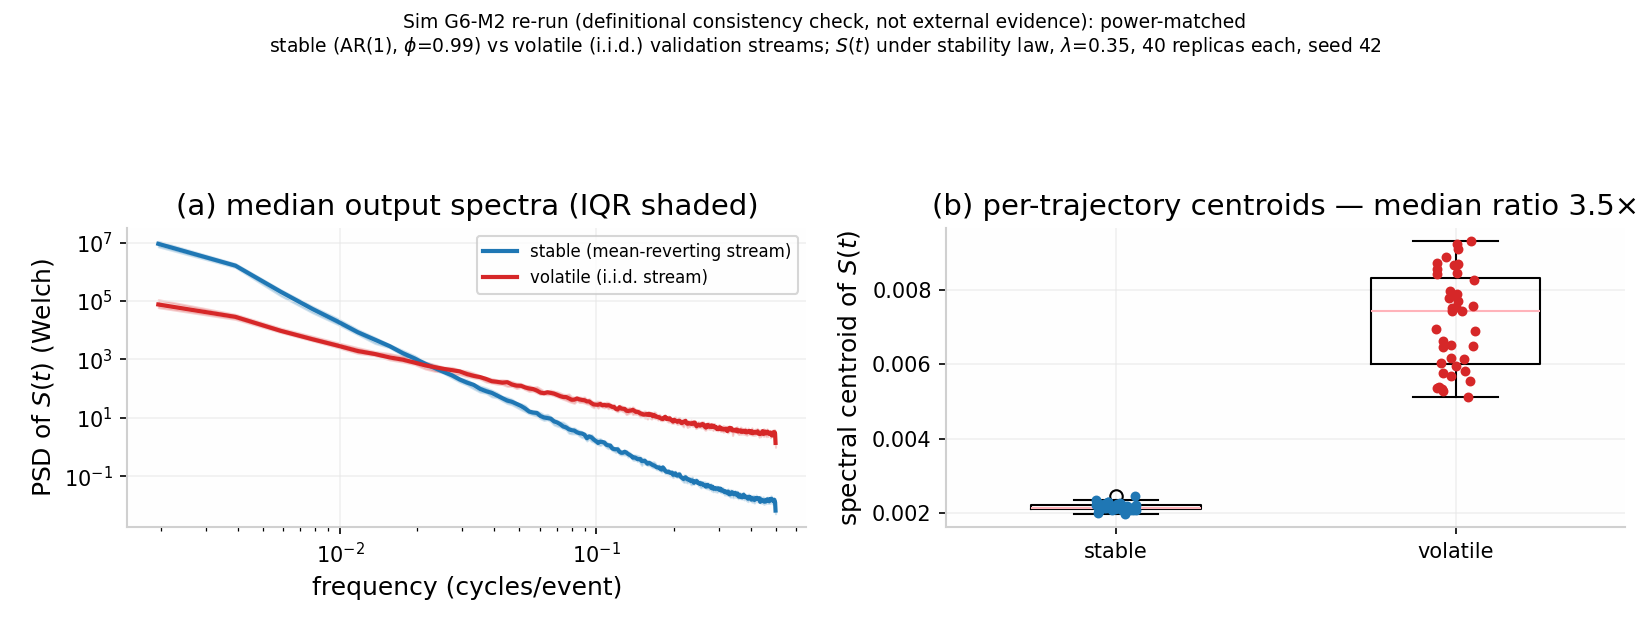
\includegraphics[width=\columnwidth]{figures/figG6_M2_spectral.png}
\caption*{\textbf{Figure S4.} Sim G6, M2 (definitional consistency check): median output power spectra of $S(t)$ and per-trajectory spectral centroids for stable versus volatile validation streams (40 replicas per condition, post-transient Welch spectra). Median centroid ratio $3.5\times$, BCa 95\% CI $[3.04, 3.69]$; complete separation (Mann--Whitney $p = 7.2 \times 10^{-15}$). A check that the stable/volatile definition is operational, not external evidence (\S 3.6).}
\end{figure}

\begin{figure}[!tb]
\centering
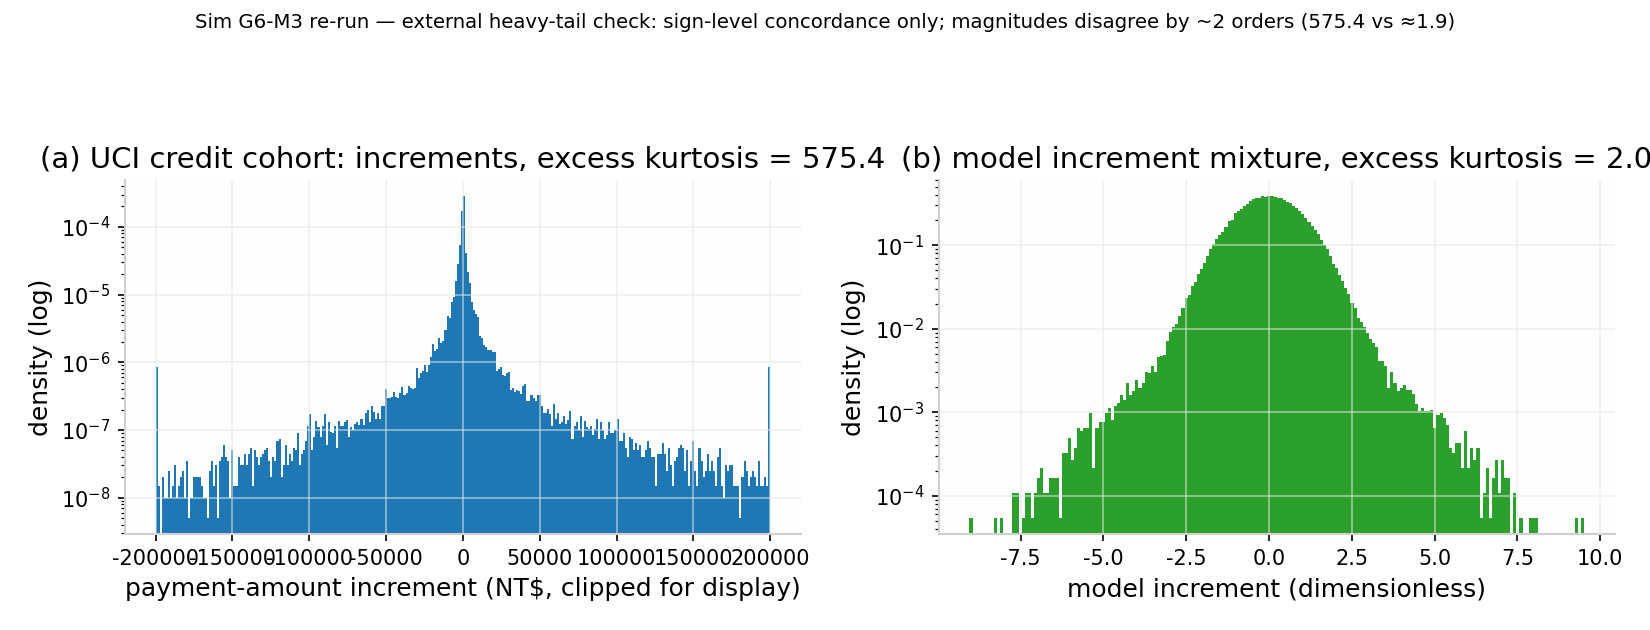
\includegraphics[width=\columnwidth]{figures/figG6_M3_heavytail.png}
\caption*{\textbf{Figure S5.} Sim G6, M3: month-to-month payment-amount increments of the UCI credit-card-default cohort (30,000 borrowers; excess kurtosis 575.43) versus a calibrated two-regime Gaussian mixture (excess kurtosis $\approx 2.0$). Sign-level heavy-tail concordance only; magnitudes disagree by roughly 2.5 orders of magnitude (\S 3.6).}
\end{figure}

\textbf{Sim G7 --- Long-run dynamics and cold start [SIMULATION].} $10^{5}$-event horizons under the three presets of the master law (disclosed parameters $\lambda^{+} = 0.005, \lambda^{-} = 0.02, \delta =$ 0.01/event, $S_{base} =$ 0.5): (i) the leak-free GTT law accumulates unboundedly under honest streams (S = 249 after $10^{5}$ events) and scars permanently from a single shock (S pinned at 10.4 after a -5 shock followed by silence) --- both pathologies of the pure integrator, per \S{}3.2; (ii) a leak toward zero decays trust to indistinguishability from absence with a 69-event half-life (theory $\ln2/\delta = 69.3,$ empirical 69) --- punishing exactly the low-activity, thin-file users a measurement architecture most needs to protect; (iii) the baseline-restoring reconciled law (the biological preset) recovers to within 10\% of baseline in 69 events after the same shock (138 and 207 events for the -10 and -20 shocks), exponentially at rate $\delta$ (simulated time-to-recovery matches the closed form at every shock size tested), converges to $S_{base}$ exactly, and re-settles boundedly after a mid-stream regime change. Honest nulls: small betrayals $(|\varepsilon| \lesssim 2.5)$ are absorbed without scarring under the reconciled law; and under purely score-proportional event rates the cold-start trap is real --- no history, no validations, no score, permanently --- so any deployment must seed a score-independent event floor (a design requirement, not a tunable parameter). These results are why \S{}3.2 presents the leak-free law as the tractable limit and the companion preprint as the biological model.

\begin{figure}[!tb]
\centering
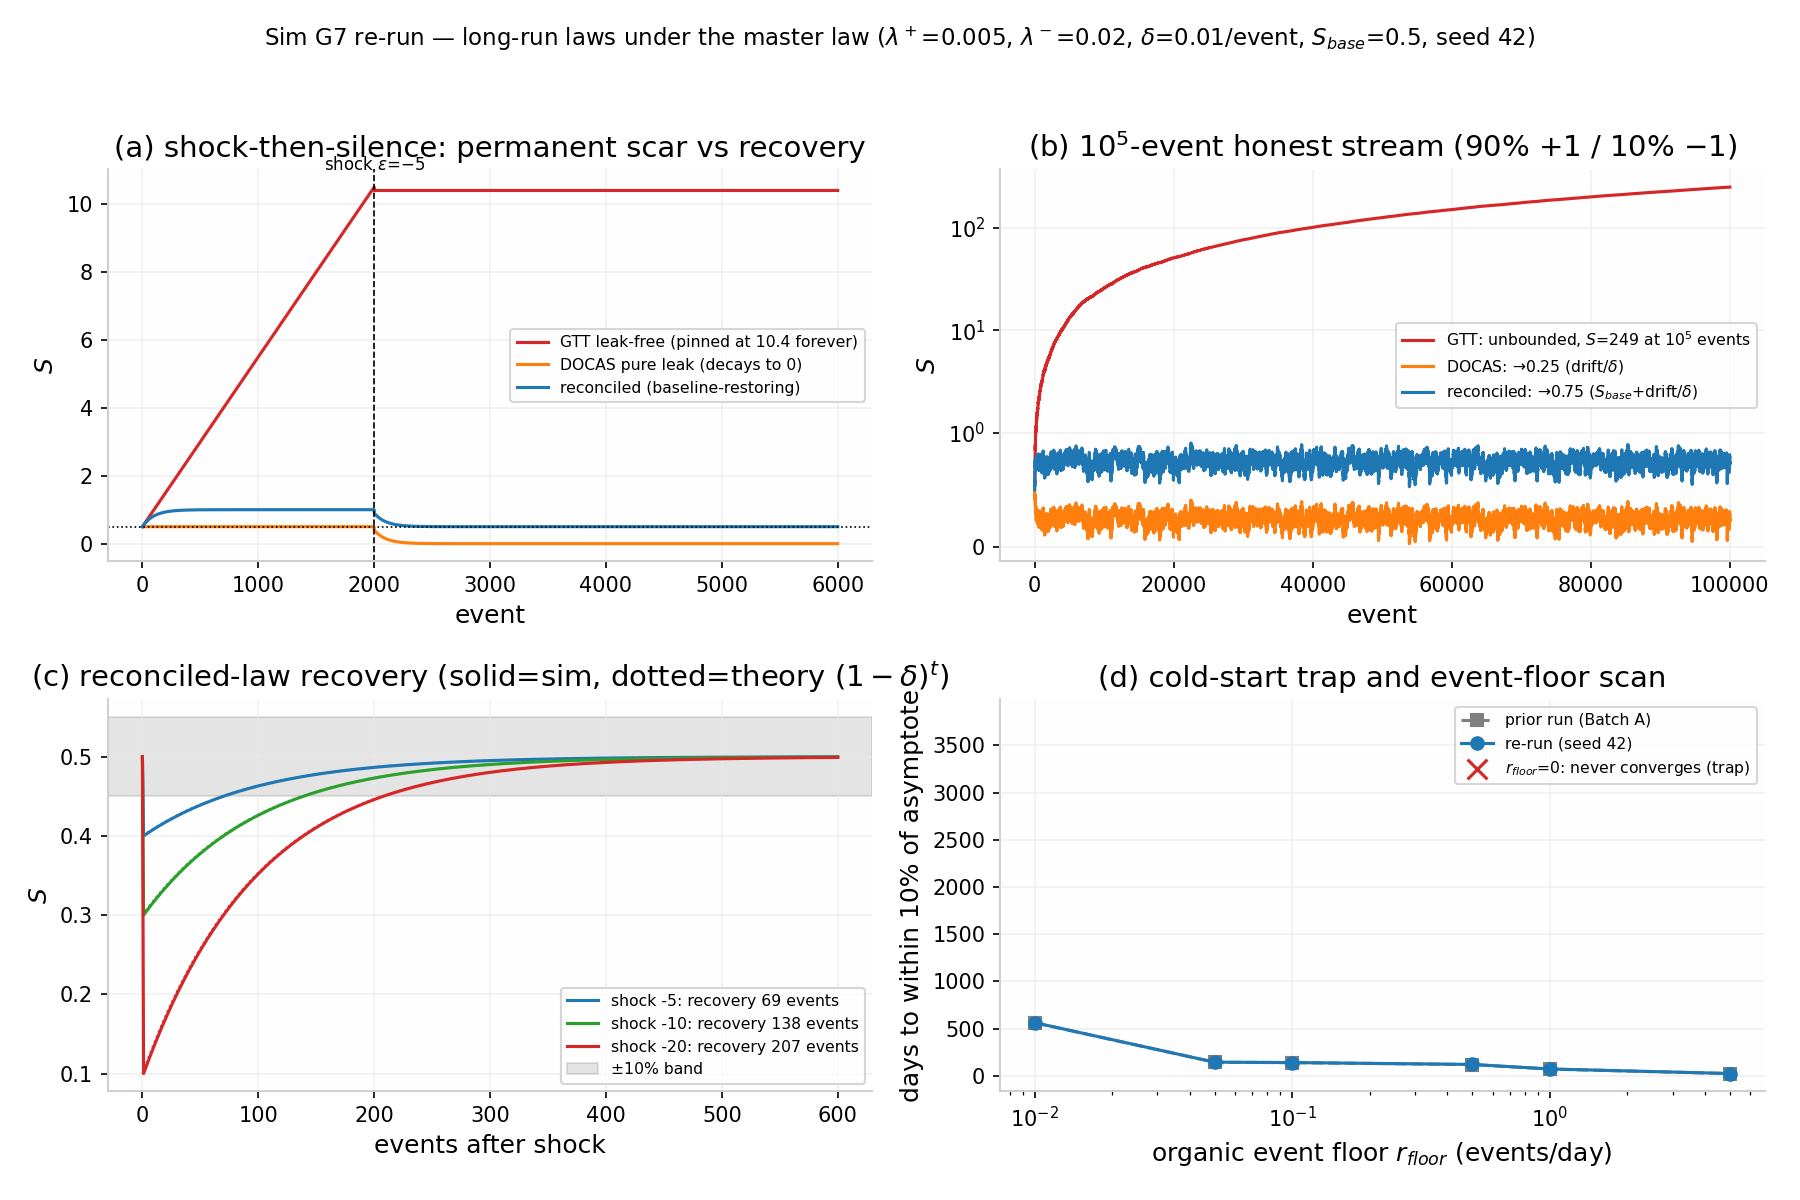
\includegraphics[width=\columnwidth]{figures/figG7_longrun.png}
\caption*{\textbf{Figure S6.} Sim G7: long-run dynamics of the three master-law presets ($\lambda^{+} = 0.005$, $\lambda^{-} = 0.02$, $\delta = 0.01$/event, $S_{\mathrm{base}} = 0.5$). Shock-then-silence, $10^{5}$-event horizons, recovery curves (69/138/207 events to within 10\% of baseline after $-5$/$-10$/$-20$ shocks under the baseline-restoring preset), and the cold-start scan (\S 3.2, \S 3.6).}
\end{figure}

\textbf{Sim G8 --- Closed-loop $\lambda$ battery [SIMULATION].} Closing the loop minimally (S feeds tomorrow's expectation, $E_{t+1} = S_t,$ per the biological loop closure; exogenous slowly varying V; GTT preset) reduces the dynamics to $x_{t+2} = x_{t+1} - \lambda x_t$ with $x = E - V,$ characteristic roots $z = (1 \pm \sqrt{1 - 4\lambda})/2.$ Verified in silico (deterministic recurrence, 118 $\lambda$ values in [0.02, 1.19], $2\cdot10^{4}$ steps): (i) the Jury stability boundary --- the closed loop is asymptotically stable iff 0 < $\lambda < 1,$ giving $\lambda$ a dimensionless natural range (theory and simulation agree to machine behavior: marginal oscillation at $\lambda = 1.00,$ divergence at $\lambda = 1.10);$ (ii) critical damping at $\lambda^{*} = 1/4$ exactly --- monotone return below, overshoot-and-ring above, with settling time minimal on the plateau $\lambda \in [0.25, 0.29]$ (simulated argmin 0.29; theory matches simulation within $\pm1$ step across the scan except near the defective double root, where the logarithmic settling formula misses the polynomial prefactor and underestimates by up to $\sim4$ steps); (iii) at $\lambda = 0.61$ the ringing period is $2\pi/\atan(\sqrt{4\lambda-1})$ = \textbf{7.17 steps predicted, 7.15 steps simulated}, with envelope decay $\sqrt{\lambda} \approx 0.78$ per step --- the falsifiable closed-loop consequence carried into \S{}6 H2. Honest null: $\lambda = 0.61$ is dynamically \emph{unremarkable} --- period and settling time vary smoothly through it (periods 7.30 / 7.23 / 7.15 / 7.10 / 7.00 at $\lambda = 0.59/0.60/0.61/0.62/0.63);$ no feature, extremum, or transition exists there. Only underdamped-branch membership, not the point value, is a falsifiable structural claim.

\begin{figure}[!tb]
\centering
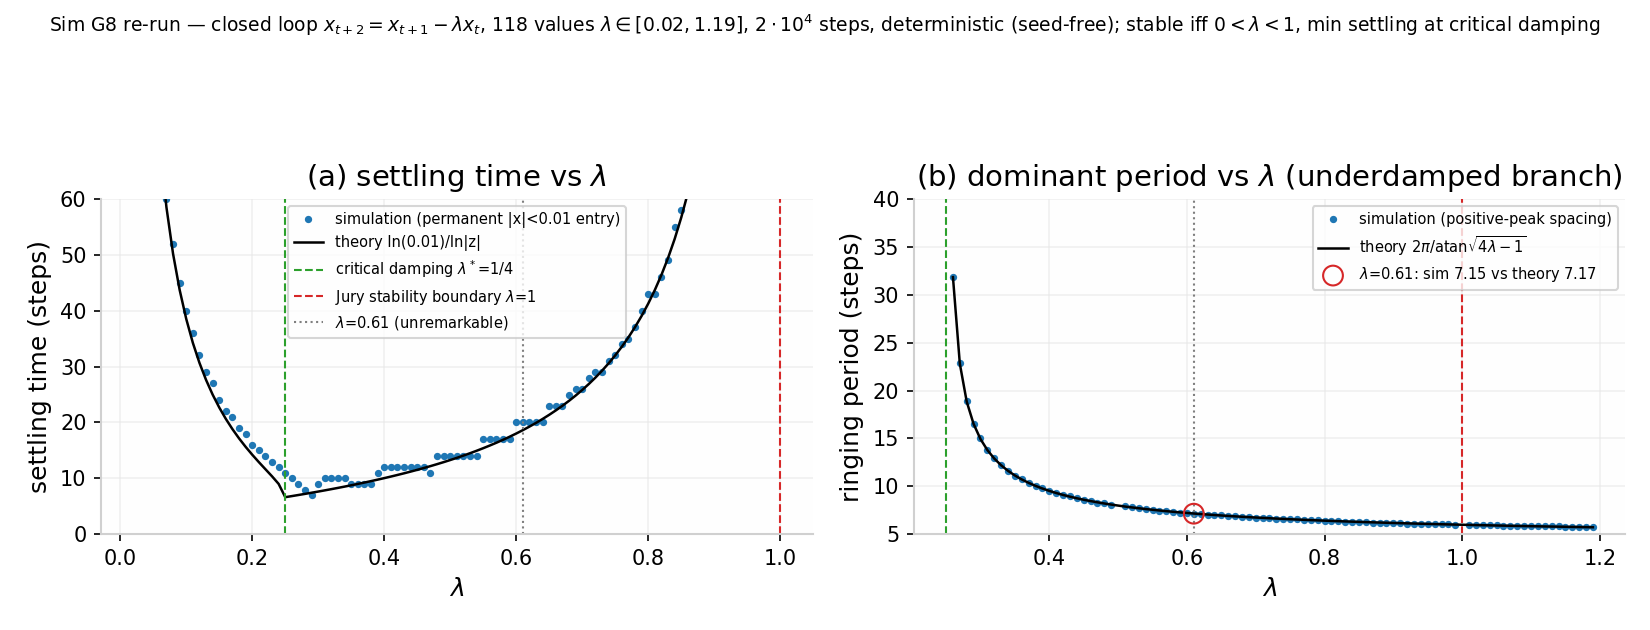
\includegraphics[width=\columnwidth]{figures/figG8_lambda_battery.png}
\caption*{\textbf{Figure S7.} Sim G8: closed-loop $\lambda$ battery. Settling time and dominant ringing period versus $\lambda$: asymptotic stability iff $0 < \lambda < 1$; critical damping at $\lambda^{*} = 1/4$, with the settling minimum on the plateau $\lambda \in [0.25, 0.29]$; ringing period $7.15$ simulated versus $7.17$ predicted at $\lambda = 0.61$ (\S 3.6).}
\end{figure}

\textbf{Sim G9 --- $\psi$ chilling-effects battery [SIMULATION].} Reported in full with the $\psi$ model in \S{}3.3: stationary variance and lag-1 autocorrelation track $\sigma^{2}/(2(\mu+\psi))$ and $e^(-(\mu+\psi))$ to within 0.8\% and $\pm0.006$ respectively across $\psi/\mu \in [-0.95, +1.00];$ distortion inflation $\times1.25 / \times2 / \times10$ at $\psi = -0.2\mu / -0.5\mu / -0.9\mu;$ residual distortion $\times1.05$ even at the illustrative best-case $\psi = -0.05\mu.$

\begin{figure}[!tb]
\centering
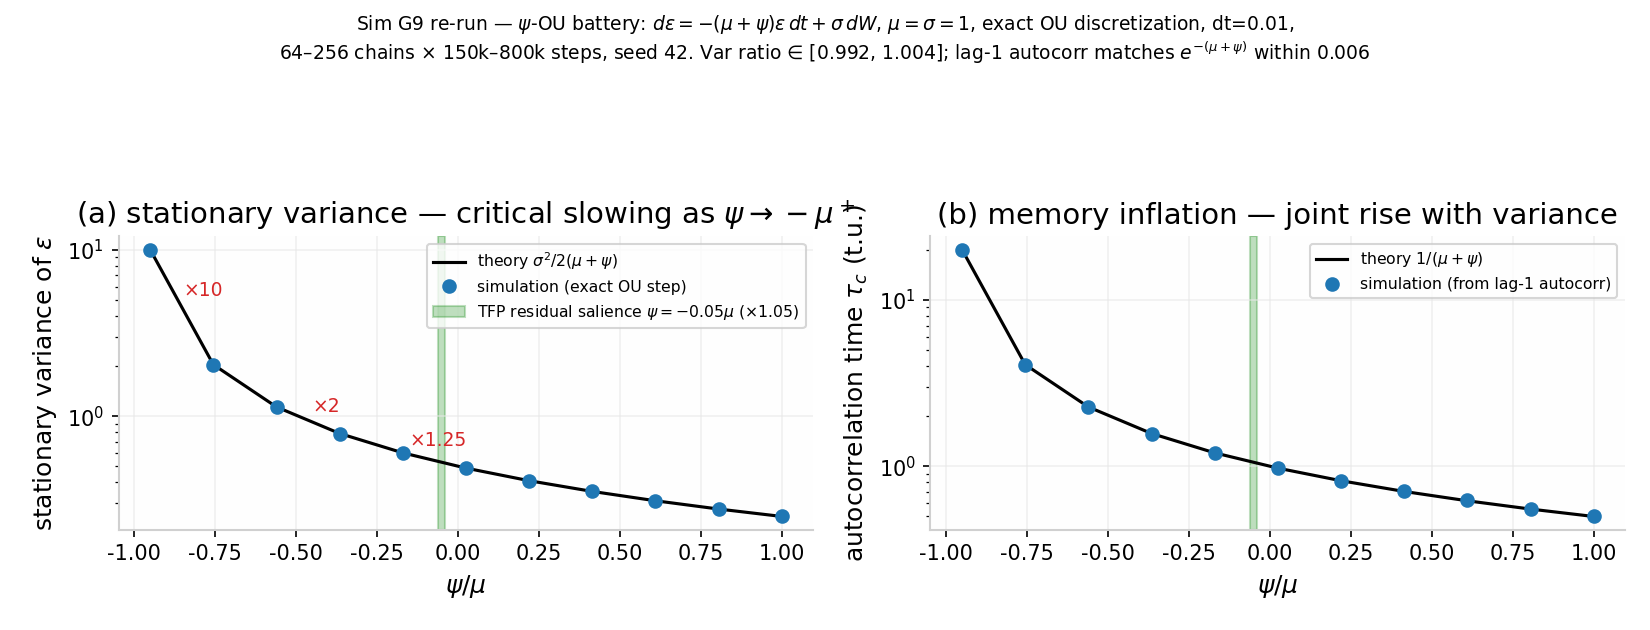
\includegraphics[width=\columnwidth]{figures/figG9_psi_battery.png}
\caption*{\textbf{Figure S8.} Sim G9: $\psi$ battery. Stationary variance and autocorrelation time versus $\psi/\mu$ with theory curves $\sigma^{2}/(2(\mu+\psi))$ and $1/(\mu+\psi)$; simulated/theory variance ratio within $[0.992, 1.004]$; the dissipation-floor-slowing asymptote as $\psi \to -\mu^{+}$ (\S 3.3, \S 3.6).}
\end{figure}

\textbf{Scope of \S{}3.6.} These results establish internal validity: the equations of \S{}2 -- 3 behave as the analysis claims, the constructs introduced above (stereographic phase map, $\psi$ model, closed-loop recurrence) are implemented as specified, and the planted-parameter recoveries are accurate. They do not establish external validity --- that is the burden of the empirical program (\S{}6).

\section*{4. Multiscale Evidence Review}

\subsection*{4.1 Behavioral genetics [EMPIRICAL]}

Twin and genomic studies converge on trust as a partly heritable, mostly polygenic trait. Cesarini et al. (2008) found significant heritability of trust-game behavior in U.S. and Swedish twin samples. The current synthesis is the Kettlewell \& Tymula (2024) meta-analysis: additive genetic factors account for approximately 33\% of variance in stated general trust (MZ twin correlation $\approx 0.36$ vs. DZ $\approx 0.16$) but only 7 -- 17\% of behavioral trust, with their own experimental estimates spanning 1 -- 37\%. Kettlewell \& Tymula's own attenuation alternative is carried with the estimate: measurement error could explain much of the stated/behavioral gap, so the gap is not clean evidence of two distinct constructs. Two consequences follow for GTT. First, the stated/behavioral gap is direct evidence that measurement instrument determines the trust quantity observed --- the empirical fingerprint of Sense 1/Sense 3 of the measurement analysis (\S{}3.5) and of the survey-instrument caveat of \S{}1.2b (Glaeser et al., 2000). Second, genetic influence enters through the mechanism level $(\lambda$ and the biological stages: dopaminergic, HPA-axis, and serotonergic function each show moderate heritability) rather than through any single ``trust gene.'' The candidate-gene literature that once claimed specific loci for trust (OXTR rs53576, AVPR1A, DRD4, COMT) has failed large-sample replication (Border et al., 2019 --- major depression; the trust-relevant candidate literature shares the same methodology and era), and this paper makes no candidate-gene claims.

\subsection*{4.2 Evolutionary game theory [EMPIRICAL]}

The strategic structure of~\eqref{eq:stability} --- cooperation maintained by feedback, degraded by noise --- recapitulates four decades of iterated-dilemma research. Axelrod's (1984) tournaments established the success of reciprocal strategies; Nowak \& Sigmund (1992) showed that in heterogeneous populations tit-for-tat can catalyze cooperation, and Nowak \& Sigmund (1993) introduced win-stay/lose-shift (Pavlov), which outperforms tit-for-tat under implementation noise because it corrects errors instead of propagating them. The definitive finite-population analysis is Imhof, Fudenberg \& Nowak (2007): under mutation -- selection dynamics with errors, tit-for-tat is never selected, but lowers the threshold above which win-stay/lose-shift fixes (cooperation selected when benefit/cost exceeds $\approx 2$) --- in their framing, tit-for-tat catalyzes the emergence of cooperation while win-stay/lose-shift is the strategy evolution settles on (paraphrase; the result, not the wording, is load-bearing). The mapping onto GTT is structural: WSLS is the strategy that re-estimates after mismatch (lose-shift = recognition + activation) and restores after validation (win-stay = stabilization); TFT's failure mode is precisely the absence of a recognition stage. Indirect reciprocity (Nowak \& Sigmund, 1998) and network reciprocity extend the same structure to populations; Fehr \& Gächter (2002) document costly punishment sustaining cooperation experimentally; Henrich et al. (2005) document its cross-cultural variability --- evidence, within GTT, that $\lambda$ is population- and culture-parameterized (and one reason no universal point value of $\lambda$ is claimed; \S{}6 H2).

\textbf{Exploitation of feedback learners.} Because the trust update conditions on reciprocal feedback, it belongs to the class of adaptive strategies that zero-determinant (ZD) players can unilaterally exploit in iterated dilemmas: Press \& Dyson (2012) proved that a memory-one player can enforce a linear relation between the two players' long-run payoffs, and that against an ``evolutionary'' opponent --- one that adapts its play to improve its own payoff, exactly what a prediction-error trust updater does --- the extortion subclass guarantees the ZD player a surplus while the adapting opponent's best response is full cooperation at a worse split. Pairwise, a purely reciprocal-feedback trust system has a \emph{proven} exploitation vulnerability. The necessary caveats, so the point is not overcorrected: extortionate ZD strategies are evolutionarily unstable --- selected against in populations (Adami \& Hintze, 2013; Hilbe, Nowak \& Sigmund, 2013) --- and evolving populations converge to \emph{generous} ZD strategies (Stewart \& Plotkin, 2013). The design consequences adopted by the stack are: (i) memory longer than one round (the theorem's premise is memory-one play); (ii) monitoring of payoff-ratio asymmetry, not only prediction error, as an extortion-detection channel; and (iii) all robustness claims in this paper are stated relative to strategy classes that exclude ZD extortion, or they fail by counterexample (\S{}7, scope limits).

\subsection*{4.3 Predictive processing and neuroeconomics [EMPIRICAL]}

Predictive-processing theory reframes perception as active inference: brains generate hypotheses about sensory input, minimizing the difference between prediction and evidence (Friston, 2010; Clark, 2013; Hohwy, 2013). Economic agents exhibit the same prediction-error update structure --- forecasting returns and adjusting behavior when expectations fail. GTT's E/V structure is this architecture applied to social expectation, and its update rule is the canonical learning rule of that architecture: the delta rule of Rescorla \& Wagner (1972), generalized to temporal-difference learning (Sutton, 1988; Sutton \& Barto, 2018) and established neurally as the dopaminergic reward-prediction-error signal (Schultz, Dayan \& Montague, 1997). Momentary subjective well-being tracks reward prediction errors: Rutledge et al. (2014) showed happiness is explained by recent expectations and RPEs (weights significant at Z > 3.3, p < 0.001), and dopaminergic transmission causally modulates even abstract aesthetic reward (Ferreri et al., 2019). Epistemic-vigilance research shows that hearers run dedicated checks on communicated information --- source-reliability and content-plausibility screening that amounts to \emph{calibrated distrust} (Sperber et al., 2010); within GTT these are recognition-stage operations that modulate the gate $r_t,$ the micro-level counterpart of ``you have to calibrate before you can trust the meaning.'' The neurochemical detail of the stage sequence is deferred to the companion biological-instantiation preprint.

\textbf{The FEP unfalsifiability critique, and how this program avoids the same charge.} Predictive-processing and free-energy frameworks have been charged with equivocating between tautological and empirical readings (Andrews, 2021), with unification by fiat --- component models mutually inconsistent, counter-evidence absorbed by post-hoc adjustment of priors and precision weights (Litwin \& Miłkowski, 2020) --- and with being a redescription schema that derives no mechanisms (Colombo \& Wright, 2017, 2021). GTT uses predictive processing as an \emph{empirical modeling framework}, and it answers the charge by construction rather than by disclaimer: (i) the theory is stated in the empirical reading only --- a specific update structure with named parameters $(\lambda, \mu, \psi,$ precisions), not a variational redescription; (ii) all precision/prior parameters are fixed a priori in the pre-registration (or fit on a training partition), and post-hoc precision adjustment after a failed prediction is forbidden by the protocol; (iii) the theory stakes risky quantitative predictions that could fail --- the $\lambda$ corridor [0.46, 0.76], the $\approx7.2$-step ringing period at the target $\lambda$ (closure-conditional, \S{}6), and the joint variance-plus-autocorrelation dissipation-floor-slowing signature of $\psi$ (\S{}6); and (iv) the empirical program commits to formal model comparison against the non-GTT alternatives on the same data --- the fixed-rate delta rule, the adaptive-$\lambda$ extension, and the Behrens-style Bayesian volatility learner (Behrens et al., 2007, 2008) --- reported as Bayes factors (or protected exceedance probabilities), not as fits (\S{}6, protocol). Where the stack uses EFE vocabulary elsewhere (the companion framework's $\tau =$ -EFE), it is adopted from Friston et al. (2015, 2017) with attribution, and any claim made with it is required to change a prediction relative to the RL baseline or be re-stated in RL vocabulary.

\subsection*{4.4 Economic and institutional evidence [EMPIRICAL]}

Trust is associated with aggregate economic outcomes: Knack \& Keefer (1997) found trust and civic norms significantly associated with growth and investment across 29 market economies --- a cross-country regression in which causality may run from institutions to both trust and growth, and the instruments are weak; we cite the association, not the causation. Zak \& Knack (2001) modeled verification investment as a costly substitute for trust --- the formal precursor of treating $V$ as something agents must sometimes pay to obtain, and of low-trust poverty traps as self-confirming low-S equilibria in which validation opportunities are never purchased. (Both literatures inherit the \S{}1.2b caveat: their regressions run on the survey item Glaeser et al. (2000) showed tracks trustworthiness; the survey-item evidence is contested (Glaeser et al., 2000) and the macro correlations are associational.) Guiso, Sapienza \& Zingales (2008) showed that individual-level trust predicts stock-market participation --- higher trust raises the probability of holding stocks and the portfolio share invested --- providing a demand-side explanation of the limited-participation puzzle. At the institutional scale, social isolation --- the chronic absence of validating feedback --- carries measurable mortality risk: meta-analytic odds of death elevated by 26\% (loneliness), 29\% (social isolation), and 32\% (living alone) (Holt-Lunstad et al., 2015); we note these are associational estimates measured on isolation cohorts and cite them as risk markers, not as links in a causal chain from trust states to mortality. Misinformation dynamics show the cost of failed validation at network scale: false news spreads farther and roughly six times faster to 1,500 people than true news on Twitter, with falsehoods $\sim70\%$ more likely to be retweeted (Vosoughi, Roy \& Aral, 2018). The institutional framing is as old as exchange itself: credit predates barter --- long before coined money, humans exchanged value through reputation-rooted obligations (Graeber, 2011) --- and behavioral economics shows that framing and choice architecture can re-anchor expectations when equilibrium fails (Kahneman \& Tversky, 1979; Thaler \& Sunstein, 2008). Herbert Simon's observation names the modern bottleneck: a wealth of information creates a poverty of attention (Simon, 1971) --- when good agents receive distorted data, they make distorted decisions, which is precisely the mismatch-accumulation pathology of \S{}3.2.

\subsection*{4.5 Connectome-scale replication across species [SIMULATION]}
\addcontentsline{toc}{subsection}{4.5 Connectome-scale replication across species}

The biological layer's connectome-scale tests live where the biology lives, in the companion connectome-scale preprint: the F1 series on the fly mushroom body (FlyWire v783; reference gate PASS, F1a INDETERMINATE-instrument, F1a2 FAIL on its frozen permutation criterion, F1b PASS --- 7/7 as frozen, criteria 6--7 at a floor-saturation calibration artifact) and Simulation H1 on MICrONS mouse visual cortex (compound FAIL: no single-class budget dominance --- median 0.313, maximum 0.360, against a 0.50 criterion --- while global partner permutation fails to abolish throughput, $R_{\mathrm{perm}} = 1.340$ against a $\geq 0.50$ retention criterion). The cross-species summary is non-abolition under global partner permutation on different metrics and criteria --- the fly retained $\approx$21\% (position-based) to $\approx$53\% (class-faithful) of the intact learning effect against an abolition criterion ($>0.95,$ failed); mouse cortex retained 134\% of throughput ($\geq 0.50,$ met) --- not a matched quantitative replication, and the single-class structural basis does not transfer. A human-cortex replication (H01, H01 dataset) is pre-registered and in progress under the same frozen criteria. Registrations, amendments, closure documents, readout CSVs, and logs are deposited at OSF (DOI: [insert]). Full protocols, criteria, and figures: the companion preprint, \S{}5.6--5.7.

\subsection*{4.6 Reality monitoring: expectation imagery corrupts the trust update in the G6-M1 model [SIMULATION]}

The update law $\Delta S_t = \lambda(V_t - E_t)$ consumes the \emph{perceived} outcome, not the veridical one. Perceptual reality monitoring --- the capacity to distinguish imagination from reality --- is known to fail in a specific, modelable way: imagery and perception are subjectively intermixed into a single signal whose strength is compared against a reality threshold, so sufficiently vivid imagination is judged real (Dijkstra \& Fleming, 2023; neural basis: Dijkstra et al., 2025; review: Dijkstra et al., 2022). Expectation vividness is not fixed, moreover: the words available to describe an anticipated outcome shape emotion percepts (Gendron et al., 2012), which by extension gives the corruption channel a plausible linguistic lever. Sim G22 (pre-registered before data; seed 20260913; 60 initial conditions on $\Delta^{4}$; $\lambda = 0.35$ planted; Hellinger-chord distances, the printed G6-M1 convention) grafts the source-mixing model onto the G6-M1 dynamics: each observer's update target is the inseparable mixture $\hat{S} = (\alpha T^{*} + v E)/(\alpha + v)$, with $E$ the imagined outcome, $v$ the imagery strength drawn from the source study's vividness distribution, and updates gated by the reality threshold $T = 2.5$.

The frozen criteria resolved as follows (Figure SR6). The instrument gate passed (Arm 0 reproduces G6-M1 in verdict --- 60/60 trajectories inside the $d < 0.05$ band at step 7, mean initial distance $\bar{d}_0 = 0.284$). Corruption is real at empirically normal imagery strength: mean final distance to $T^{*}$ is 0.197 at the source study's sample mean ($\mu_v = 2.5$) and 0.229 at $\mu_v = 5.0$, far outside the band, with trajectories captured by their imagined targets ($\langle d(\theta, E)\rangle < \langle d(\theta, T^{*})\rangle$). The dependence on imagery strength is non-monotone, with the corruption minimum at that sample mean: the zero-imagery baseline fails the band as well --- at $\mu_v = 0$ the ungated observers end at mean distance 0.275 under both outcome regimes, 92\% of steps producing no update under dense outcomes, because without imagery the mixed signal never crosses the reality threshold and the gate blocks nearly every update. The mixture weight $\alpha = 1.0$ relative to the reality threshold $T = 2.5$ is a modeling choice, not an empirical estimate. Both predicted failure modes occur: weak-imagery observers explain genuine evidence away (57\% of steps produce no update at $\mu_v = 1.25$ --- stagnation), and under sparse outcomes 48\% of updates at $\mu_v = 5.0$ are driven by hallucinated outcomes. The system-side defense --- aggregating eight independent channels --- attenuates the corruption $\approx$$2.9\times$ but fails its frozen restoration criterion (0.079 > 0.05), and under shared expectations (a formalized collective illusion) the rescue collapses entirely (0.239). Compound verdict: FAIL, reported as such --- the honest summary is that aggregation helps only against idiosyncratic distortion, not against a shared one. Nothing here is a claim about human trust dynamics: the vividness distribution is imported from a visual-perception study, $\lambda$ is planted, and the human analog is prospective (\S{}6's registered program now has a stated reason to record imagery vividness as a covariate).

\begin{figure}[!tb]
\centering
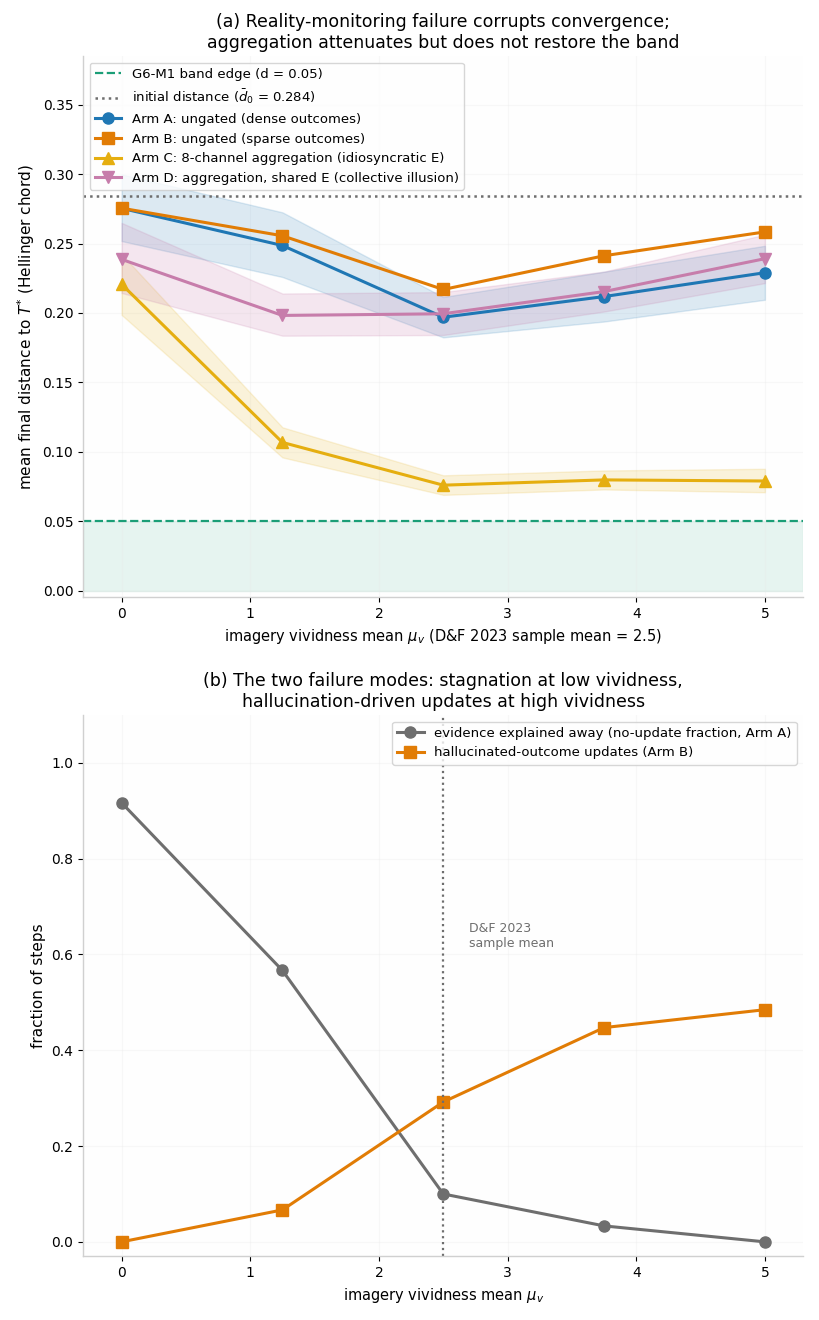
\includegraphics[width=\columnwidth]{figures/figG22_reality_monitoring_column.png}
\caption*{\textbf{Figure SR6.} Reality-monitoring corruption of trust-stage dynamics (Sim G22, seed 20260913; pre-registered frozen criteria). (a) Mean final distance to the true target $T^{*}$ across the imagery-vividness grid: ungated observers (dense and sparse outcome regimes) sit far outside the G6-M1 convergence band (green) at and above the source study's sample mean (2.5); eight-channel aggregation attenuates the bias $\approx$$2.9\times$ but does not restore the band, and fails entirely when expectations are shared (collective-illusion arm). Shaded ribbons: 95\% bootstrap CIs. (b) The two failure modes: evidence explained away (stagnation) at low vividness; hallucinated-outcome updates under sparse outcomes at high vividness. Verdicts per frozen criteria: C1--C4, C6 PASS; C5 FAIL; compound FAIL. Pre-registration, closure note, code, and results JSON in the deposit.}
\end{figure}

\section*{5. The Manifestation Chain [HYPOTHESIS --- levels 2--3]}

The stack's thesis is that one vector state and update law recurs at three levels (level 1 is the formal object; levels 2--3 are hypothesized instantiations, each carried by its companion preprint as a pre-registered, falsifiable claim):

\begin{quote}\noindent GTT vector $T$ (formal object) $\to$ biological instantiation (a five-channel neuromodulatory architecture --- D,O,C,A,S functional roles, not a serial cascade) $\to$ behavioral manifestation (a domain-agnostic measurement architecture: verifiable interactions as validations) $\to$ financial application (specified separately)\end{quote}

Financial behavior is singled out among behavioral domains for three principled reasons: outcomes are binary or near-binary (obligation met or not), the validation is immediate and recorded, and the expectation scale is directly estimable --- outcomes are recorded in dollars, so the normalized mismatch $\tilde{\varepsilon} = (V - E)/s_{fin}$ (Definition 2a) is objectively computable with $s_{fin}$ the dollar-RMSE of the predicted outcome distribution. Finance is the domain where the Definition 2a normalization is least contestable; that --- not any slogan about dollars --- is the principled reason it is the first application. Physiological streams (heart-rate variability, sleep, activity) and financial streams are dual measurement layers on the same latent process, each scored against the biological instantiation's theory. In the financial application, physiological data are used to validate the theory's stage assignments --- never as credit-decision inputs.

\section*{6. Proposed Empirical Program}

All language in this section is prospective. No results are reported; the studies are designed and pre-registered before data analysis. All precision/prior parameters are fixed a priori (or fit on a training partition); post-hoc adjustment of precisions after a failed prediction is forbidden by protocol (\S{}4.3).

\textbf{Hypothesis R1 (registered program hypothesis --- stability law; distinct from the \S{}1.1 theory hypothesis H1).} In repeated-interaction data with recorded expectations and outcomes, $\Delta S_t$ (operationalized via the biological stage markers) follows equation~\eqref{eq:stability} with subject-specific $\lambda_i.$ Here $H_t$ denotes the observable stabilization readout (the biological stage-marker composite proxying S), distinct from the latent state. Estimation: state-space form

\begin{equation}
\begin{split}
\text{Observation: } & \Delta H_t = \lambda_H \varepsilon(t) + u_t;\\ \text{State: } &S_t = S_{t-1} + \lambda \varepsilon(t-1) + \eta_t
\end{split}
\label{eq:statespace}
\end{equation}

(with $\varepsilon$ in the stack-wide V - E convention of Definition 2) fit by Kalman filtering / EM, and a Bayesian hierarchical variant $\lambda_{H,i} \sim \mathcal{N}(\mu_\lambda, \tau_\lambda^{2})$ reporting the population posterior $\mu_\lambda$ and individual heterogeneity. $\lambda_H \equiv \lambda$ under the proxy assumption $H_t = S_t + {}$measurement noise; if the readout carries its own gain, the H2 estimand is the state coefficient $\lambda$ and $\lambda_H$ is a nuisance parameter --- the registration names which.

\textbf{H2 (Target coefficient).} The population mean trust-sensitivity is pre-registered as the target $\mu_\lambda = 0.61$ with an \textbf{equivalence corridor [0.46, 0.76]}. The point value 0.61 is a target hypothesis, not an estimate and not a derived quantity: \textbf{no derivation of its value from the theory is claimed.} The target value 0.61 is the author's prior estimate with no origin beyond anchoring the registration; no derivation is claimed, and the simulation battery shows no dynamical feature at that value --- its role is to anchor registration, and the estimate stands or falls on the data. The corridor half-width 0.15 is a pre-registered smallest effect size of interest (SESOI) for an equivalence test --- a substantive choice, not instrument resolution: the instrument's demonstrated recovery error is far finer (the stack's estimator pipeline, estimator-validation run reported in the financial application preprint: mean 0.0074, p95 0.0215, max 0.0343; ultra-thin worst case 0.0737), so the corridor is conservative in the direction of easy corroboration --- and H2 corroboration is therefore weak evidence; the primary test is the model comparison against the adaptive-$\lambda$ (Behrens-style) alternative in (iii) below. The structural-misspecification battery below (SIM-R1, run) shows this is load-bearing, not rhetorical: corridor corroboration is achievable by misspecification bias alone. H2 is corroborated if the hierarchical posterior for $\mu_\lambda$ concentrates inside the corridor at the 95\% highest-density credible level (fixed in the registration); it is refuted by any of: (i) the posterior excludes [0.46, 0.76]; (ii) cross-domain measurement invariance fails --- financial, social, and physiological streams returning population means that differ by more than the corridor width after per-domain normalization (Definition 2a) --- showing 0.61 to be a property of one instrument; (iii) the constant-$\lambda$ state equation fails posterior predictive checks against an adaptive-$\lambda$ extension.

\textbf{Open identification note --- the $\lambda \cdot r_t$ product confound.} From the $S$ series (or its readout $H$) alone, the trust-sensitivity $\lambda$ and the recognition gate $r_t$ enter the master law only as the product $\lambda \cdot r_t$: an ungated stream with sensitivity $\lambda$ and a gated stream with mean gate $\bar{r} < 1$ and sensitivity $\lambda/\bar{r}$ generate identical update sequences. Time-varying gating is a gain variation of exactly the class the SIM-R1 misspecification battery shows the certified constant-gain estimator misrecovers (the $\varepsilon^{2}$-weighted gain, not the time average), so $\lambda$ is not separately identifiable from field $S$/$H$ data without additional structure. Field identification of $\lambda$ therefore requires either (a) a separately identified C-channel gate readout (the biological recognition-marker composite, measured independently of the update) or (b) the registered model comparison of this section, with the product confound disclosed. This is stated as an open identification note; no resolution is claimed. Path (a) presupposes a validated recognition readout, which the companion preprint's registered carrier gate (GATE-1) has not yet delivered, so (b) is the operative path.

\textbf{Structural-misspecification battery (SIM-R1 battery 1, run; [SIMULATION]).} The registered follow-up to the estimator's corridor certification has been run, and the constant-$\lambda$ estimator fails it in exactly the registered way. Under a Behrens-style adaptive-$\lambda$ ground truth (volatility-linked gain $\lambda_t = \lambda_0(1 + c\,\nu_t)$ with centered EWMA volatility statistic $\nu_t,$ $c = 1.5,$ clip non-binding, $\mathbb{E}[\lambda_t] = \lambda_0$ exactly; $N = 300$ users with cadence, sign mixture, tails, and the deliberately misspecified Gaussian fit matched to the prior battery; population time-average $\bar{\lambda} = 0.355),$ the certified constant-$\lambda$ Kalman/EM pipeline does \textbf{not} recover the time-average gain within the 0.15 corridor: $|\hat{\lambda} - \bar{\lambda}|$ mean 0.117, p95 0.255, max 0.556, with 65 of 300 users (21.7\%) outside the corridor and a systematic \emph{upward} signed bias (mean $+0.117$) --- the gain is high precisely when $|\varepsilon|$ is large. The failure is a target failure, not an arithmetic failure: against the $\varepsilon^{2}$-weighted gain $\bar{\lambda}_w = \Sigma\lambda_t\varepsilon_t^{2}/\Sigma\varepsilon_t^{2}$ the same estimator is exact (mean 0.0041, max 0.028, 0/300 outside) --- a constant-gain least-squares/Kalman fit identifies the $\varepsilon^{2}$-weighted mean gain, not the time average --- and more data does not fix it (error correlates with per-user gain dispersion, $r = 0.68,$ not with $1/n,$ $r = -0.02$). The corrosive corollary for H2: at adaptive truth $\bar{\lambda} = 0.355$ the population estimate lands at $\hat{\lambda} = 0.472$ --- \textbf{inside} the corridor [0.46, 0.76] while the truth lies outside it. Corridor corroboration under structural misspecification is therefore achievable purely by weighting bias, which is why the Behrens model comparison of criterion (iii) --- already the stated primary test --- is load-bearing, not optional. The bias is approximately linear in the volatility coupling $c$ (population bias / corridor-breach fraction: $+0.060$ / 3.7\% at $c = 0.75;$ $+0.117$ / 21.7\% at $c = 1.5;$ $+0.211$ / 66.7\% at $c = 3.0),$ and the constant-truth replication control passes at its certified error (mean 0.0042, p95 0.0119, max 0.0208, 0/300 outside): the estimator performs as certified exactly when the truth shares its structure. The two-gain $(\lambda^{+}, \lambda^{-})$ variant is no better as an asymmetry instrument: it detects asymmetry direction reliably (AUC 0.968 against the symmetric-adaptive control) but inflates magnitude (recovered ratio 2.84 against a true time-average ratio of 2.00 --- the estimator nails the channel-wise $\varepsilon^{2}$-weighted ratio 2.845; the 2.0 structural reading is the artifact), and under a symmetric-but-volatility-linked truth it reports \textbf{spurious asymmetry} (ratio mean 1.41, p95 2.23). An estimated $\lambda^{-} > \lambda^{+}$ therefore cannot, by itself, distinguish TFP's structural break/build asymmetry from symmetric volatility-linked gain (Figures SR3--SR4; battery bundled with the Supporting Document (deposit pending), seed 42).

\begin{figure}[!tb]
\centering
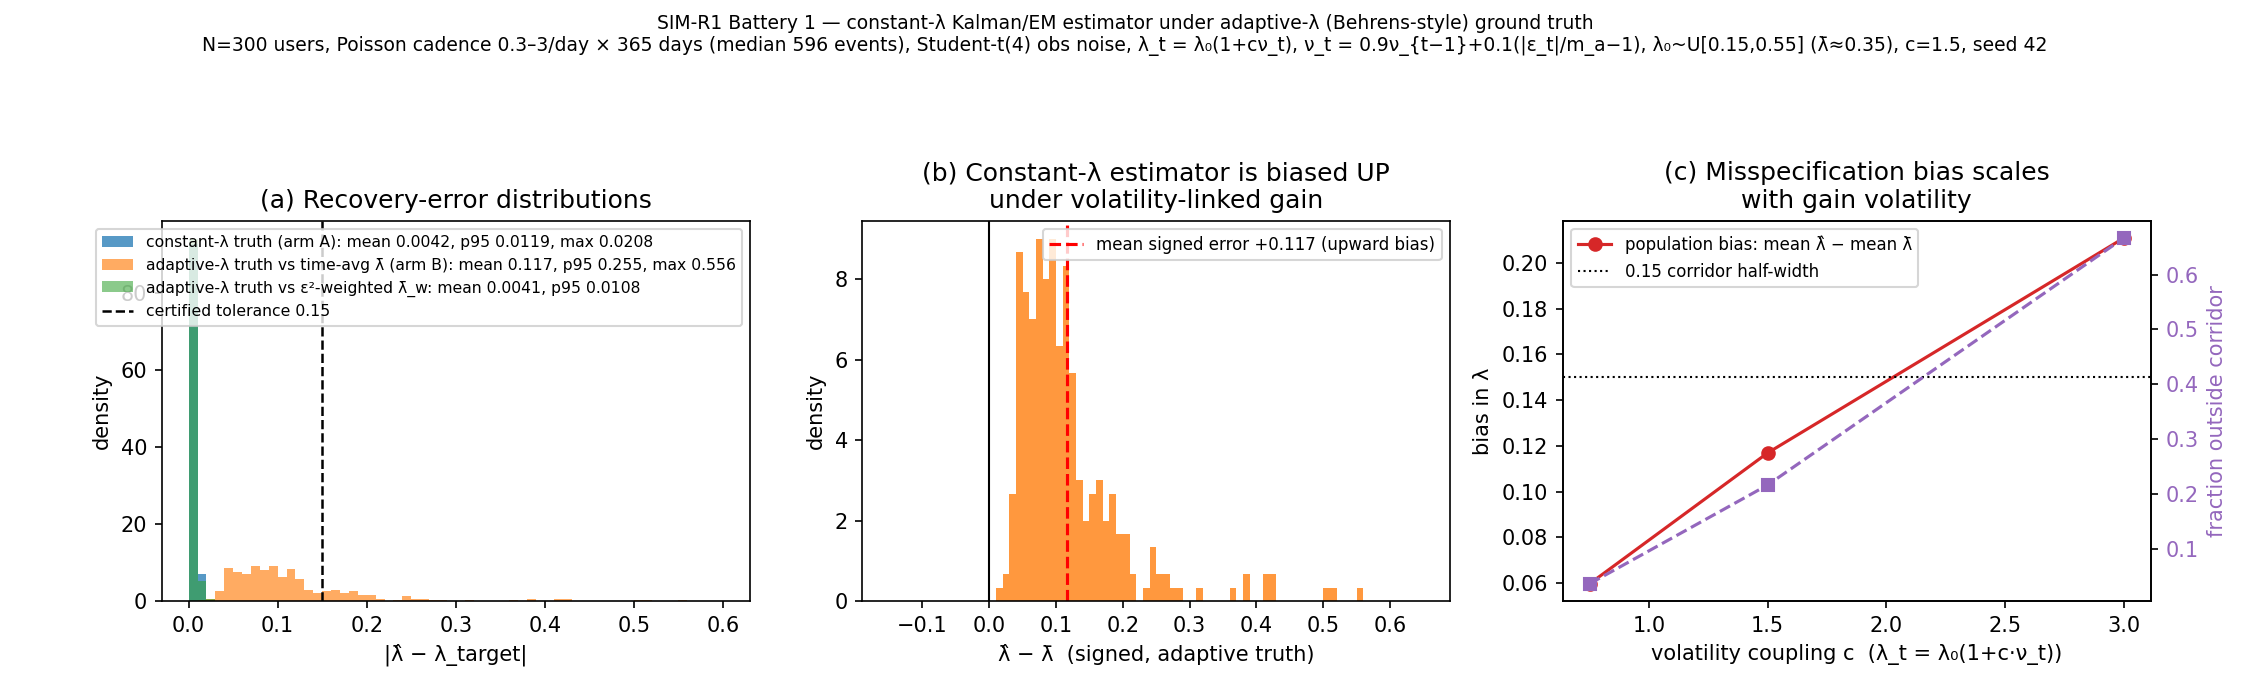
\includegraphics[width=\columnwidth]{figures/figR1_error_distributions.png}
\caption*{\textbf{Figure SR3.} SIM-R1 battery 1 ($N = 300$, seed 42): (a) $|\hat{\lambda} - \lambda_{\mathrm{target}}|$ under constant truth (mean 0.0042), adaptive truth against the time-average $\bar{\lambda}$ (mean 0.117; 21.7\% outside the 0.15 corridor), and adaptive truth against the $\varepsilon^{2}$-weighted $\bar{\lambda}_w$ (mean 0.0041); (b) signed error showing the $+0.117$ upward bias; (c) population bias and corridor-breach fraction versus volatility coupling $c \in \{0.75, 1.5, 3.0\}$ (\S 6).}
\end{figure}

\begin{figure}[!tb]
\centering
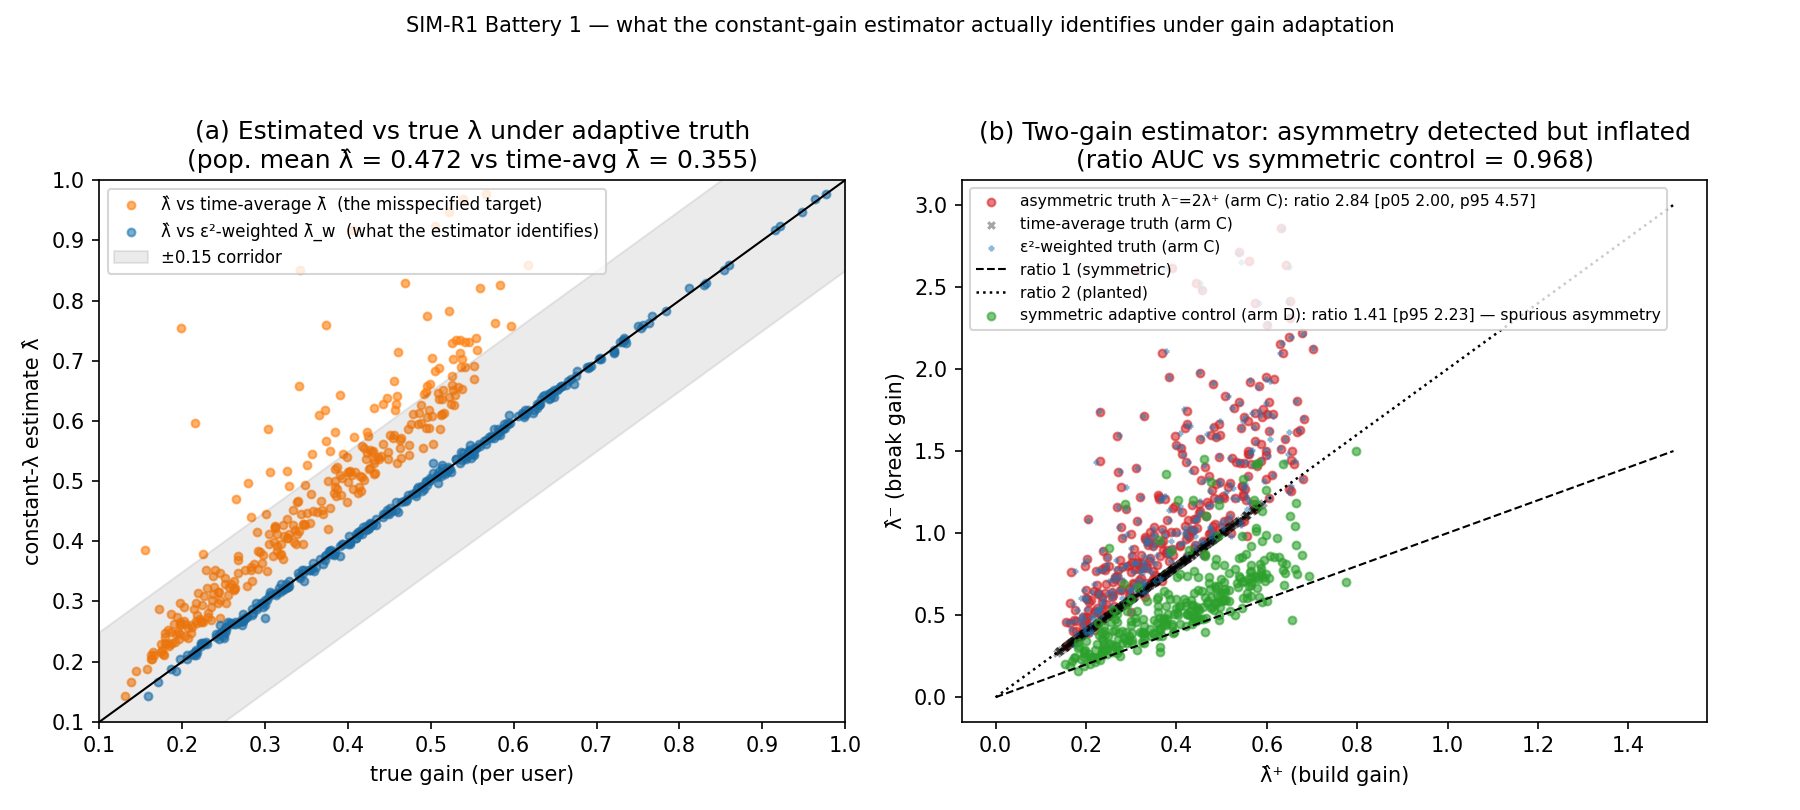
\includegraphics[width=\columnwidth]{figures/figR1_scatter_adaptive.png}
\caption*{\textbf{Figure SR4.} SIM-R1 battery 1: (a) $\hat{\lambda}$ versus the time-average $\bar{\lambda}$ and versus the $\varepsilon^{2}$-weighted $\bar{\lambda}_w$ with the $\pm 0.15$ corridor; population mean $\hat{\lambda} = 0.472$ versus $\bar{\lambda} = 0.355$ --- inside the H2 corridor while the truth lies outside. (b) Two-gain scatter: asymmetric truth $\lambda^{-} = 2\lambda^{+}$ (recovered ratio 2.84; weighted-truth ratio 2.845) versus the symmetric-adaptive control (spurious ratio mean 1.41, p95 2.23); direction AUC 0.968 (\S 6).}
\end{figure}

\textbf{Invariance hypotheses (replacing any ``universal constant'' framing).} H2a --- \emph{measurement invariance}: $\hat{\lambda}$ is equal across domains after dimensionless normalization, up to the corridor. H2b --- \emph{rank-order stability}: the ordering of individuals' $\lambda_i$ is stable across domains and across repeated measurement windows, even if levels drift. H2a/H2b, not point equality across settings, are the theory's consistency claims. (The cadence caveat applies: a per-event $\lambda$ and a per-unit-time $\lambda$ are the same parameter only if event rates are stationary and stated; the pre-registration fixes the observation cadence per domain so the dimensionless $\lambda's$ are commensurable.)

\textbf{The falsifiable closed-loop consequence (from Sim G8).} Under the minimal loop closure $E_{t+1} = S_t,$ the trust dynamics reduce to $x_{t+2} = x_{t+1} - \lambda x_t:$ stable iff 0 < $\lambda < 1,$ critically damped at $\lambda^{*} = 1/4,$ and underdamped --- overshoot-and-ring after betrayal events --- above it. At the target $\lambda = 0.61$ the predicted ringing period is $2\pi/\atan(\sqrt{4\lambda-1}) \approx 7.2$ steps (7.17 predicted; the recurrence's roots are the prediction, so the in-silico 7.15 of Sim G8 is an implementation check, not corroboration), with damping envelope $\sqrt{\lambda} \approx 0.78$ per step. The pre-registered prediction is therefore \emph{behavioral}, not numerological: following signed mismatch events in repeated-interaction data, $S$ (read off H) should overshoot and oscillate with a period set by $\hat{\lambda}$ via the stated formula, decaying at $\sqrt{\hat{\lambda}}$ per step. We state plainly: \textbf{0.61 is otherwise nothing special} --- period and settling time vary smoothly through it with no feature, extremum, or transition (Sim G8); only underdamped-branch membership and the period-versus-$\hat{\lambda}$ functional relation are falsifiable. A population recovered in the overdamped branch $(\lambda < 1/4),$ or ringing whose period fails the formula, refutes the structural claim independently of the point target. The $\sqrt{\lambda}$ envelope decays 0.78/step at $\lambda = 0.61$ --- the ringing is one overshoot plus a $\sim$17\% rebound, in event-index time; under realistic irregular cadence (0.3--3 events/day) detection requires the power analysis registered in the pre-registration; if underpowered, the ringing prediction is falsifiable in principle but unresolved by the proposed instruments, and that outcome would itself be reported.

\textbf{Closure sensitivity of the ringing signature (SIM-R1 battery 2, run; [SIMULATION]).} The closure dependence flagged in \S{}7 is quantified here, and the verdict is: \textbf{qualitatively robust, quantitatively closure-fragile.} Under exponential-smoothing closures $E_{t+1} = \alpha S_t + (1-\alpha)E_t$ (exact characteristic equation $z^{2} - (2-\alpha)z + (1 - \alpha(1-\lambda)) = 0;$ ringing iff $\lambda > \alpha/4;$ stable for all $0 < \alpha \leq 1,$ $0 < \lambda < 1$), the overshoot-and-ring signature survives at \emph{every} $\alpha \in (0, 1]$ at $\lambda = 0.61$ and becomes \emph{more} persistent (envelope $0.78 \to 0.96$ per step; visible cycles $1.7 \to 4.2$) --- but the period drifts smoothly: $7.17 \to 8.24 \to 9.76 \to 12.22 \to 17.65$ steps as $\alpha$ runs $1.0 \to 0.2$ (theory and simulation agree to peak-spacing quantization). The registered formula $P(\hat{\lambda}) = 2\pi/\atan(\sqrt{4\hat{\lambda}-1})$ is therefore the $\alpha = 1$ member of a family $P(\lambda, \alpha);$ testing the formula without verifying the closure tests the wrong curve. The zero-delay closure $E_t = S_t$ destroys ringing entirely (monotone return, 0.39 per step): the signature is a property of the \emph{lagged} closure, not of the update law alone. Under the two-step-delay closure $E_{t+1} = S_{t-1}$ ($z^{3} - z^{2} + \lambda = 0$) the system rings at period 10.04 but the stability boundary moves from 1 to exactly $(\sqrt{5}-1)/2 = 1/\varphi = 0.618034$ (Jury/bisection, confirmed to machine precision): the target $\lambda = 0.61$ sits $1.30\%$ below that boundary, the ringing is nearly undamped (envelope 0.9962 per step, $\sim$79 visible cycles), and $\lambda = 0.63$ would diverge --- the closed-loop stability margin claimed for the target ($(0,1),$ \S{}3.6 Sim G8) shrinks to $(0, 0.618)$ under this closure. We record, without interpretation and claiming no significance for it, the numerical coincidence that the H2 target sits just below the exact boundary $1/\varphi$ under this one closure; the boundary is closure-dependent and no dynamical feature at 0.61 is claimed anywhere. Consequence for the empirical test: the falsifiable content ``period set by $\hat{\lambda}$ via the stated formula'' is true \emph{conditional on the minimal closure}; an empirical ringing test must either verify the closure (estimate the $E$-mapping) or register the family $P(\lambda, \alpha)$ and joint-fit $(\lambda, \alpha)$ --- an observed failure of the 7.17-step period would not discriminate ``wrong $\lambda$'' from ``wrong closure.'' One detectability note cuts the other way: smoothing closures \emph{increase} ring persistence (more visible cycles), so closure uncertainty is bad news for the period formula, not for detection itself.

\textbf{H2 identification plan (what would move $\lambda$ off 0.61).} $\lambda$ is identified from the impulse response of $S$ to signed mismatch events: in the state-space form above it enters as the coefficient on $\varepsilon(t-1)$ in the state equation, so identification requires within-subject variation in $\varepsilon_t$ conditional on $S_{t-1}$ --- events in which expectation and validation diverge by a recorded, exogenous amount (the companion preprint's offer-stimulus paradigm is designed to generate exactly such variation). Three pre-registered outcomes count against H2: (i) the hierarchical posterior $\mu_\lambda$ excludes the corridor at the 95\% highest-density credible level (fixed in the registration); (ii) $\lambda$ estimates fail cross-domain measurement invariance, which would show that 0.61, if recovered anywhere, is a property of one instrument rather than of trust dynamics; (iii) the constant-$\lambda$ state equation fails posterior predictive checks against an adaptive-$\lambda$ extension, in which case any point prediction is moot. H2 is corroborated only if the posterior concentrates inside the corridor and passes invariance across streams --- a corridor whose half-width is a pre-registered smallest effect size of interest (SESOI), far coarser than the estimator's demonstrated recovery error, so corroboration inside it is weak evidence and the primary test is the model comparison in (iii).

\textbf{H0a test (registered).} Estimate the $\iota$-projected process from multi-channel trust time series; test strong lumpability (Kemeny--Snell $Q \cdot A \cdot P \cdot Q = P \cdot Q$) via non-Markovianity of the projection and hysteresis at fixed $\iota$; rejection of lumpability corroborates H1's vector-necessity claim. The test requires measurable channel activities --- if stage activities prove unmeasurable (\S{}3.1 fallback), H0a is untestable on the current instruments and this limitation is stated.

\textbf{H3 (Phase transition).} Trust networks parameterized by feedback quality will exhibit the Kuramoto-\emph{form} threshold of Section 3.4: below a critical coupling (feedback bandwidth/latency), collective PAS collapses toward zero independent of mean individual dispositions. Consistent with \S{}3.4, the pre-registered prediction is the functional form --- a continuous onset of PAS coherence at a critical feedback quality --- not the mean-field number $K_c = 2/\pi g(0),$ which on sparse, weighted real networks requires network corrections (\S{}7).

\textbf{H4 (Measurement dependence).} Salient observation of the measurement process itself will shift the effective dissipation of the mismatch stream --- the behavioral observer effect, formalized as $\psi(m)$ in \S{}3.3. The falsifiable signature is the joint movement of the two derived statistics: \textbf{rising stationary variance $\sigma^{2}/(2(\mu+\psi))$ together with rising lag-1 autocorrelation of the mismatch stream} (dissipation-floor slowing as $\psi \to -\mu^{+};$ verified in silico in Sim G9, with inflation factors $\times1.25 / \times2 / \times10$ at $\psi = -0.2\mu / -0.5\mu / -0.9\mu).$ Direction and magnitude are predicted per agent from baseline vigilance markers. The chilling-effects literature (Penney, 2016: statistically significant -19\% immediate traffic reduction to privacy-sensitive Wikipedia articles after the June 2013 surveillance revelations, with a persistent trend change in an interrupted time-series design) demonstrates the phenomenon at population scale; H4 is its trust-dynamics form. The study's own instruments are subject to the same axiom: no measurement in this program, including the stack's own protocol, achieves $\psi = 0$ (\S{}3.3), and residual-salience controls are included in the design. Two identification constraints are stated explicitly. First, $\psi$ enters every observable only through the sum $\mu + \psi$, so a salience effect is not separately identifiable from a single condition: attribution requires an exogenous salience manipulation and a baseline condition, with the effect read off the joint change in the two statistics. Second, the H4 statistic is computed in raw units, with $s_d$ held fixed across salience conditions, so that no rescaling of the expectation axis can mimic or mask a change in dissipation.

\textbf{Model-comparison commitment.} On the same repeated-interaction data, the program will fit and formally compare: (a) the GTT fixed-$\lambda$ delta rule (the Rescorla -- Wagner limit of the master law); (b) the adaptive-$\lambda$ extension; and (c) a Behrens-style hierarchical Bayesian learner with volatility-sensitive learning rate (Behrens et al., 2007, 2008) --- the established superior account of human social learning, which is treated here as a competitor to beat, not as background. Comparison is by Bayes factors (or protected exceedance probabilities), pre-registered, with all hyperparameters fixed a priori. If (c) dominates (a) decisively, the fixed-$\lambda$ theory is retained only as a tractable approximation and H2 is moot per criterion (iii) above.

\textbf{Multiplicity, stated as a program limitation.} R1, H0a, H2, H3, and H4 are tested on partly disjoint data and instruments and are registered as separate confirmatory families; no cross-hypothesis error-rate control is currently specified. The registration will fix per-hypothesis $\alpha$ and additionally report a descriptive family-wise picture (Bonferroni and BH over the primary tests); no adjusted claim is made in this paper.

\textbf{Protocol.} The companion protocol's financial application implements the measurement infrastructure; the companion experiment's stage mapping (D=expectation, O=validation, C=recognition, A=activation, S=stabilization) is frozen by pre-registration (OSF) before any data are analyzed. Power analyses and exclusion criteria are specified in the pre-registration documents.

\section*{7. Discussion}

\textbf{What the theory claims.} Trust is a measurable relation between expectation and validation; its stabilization dynamics obey the Rescorla -- Wagner limit of a master update law whose alignment manifold $E = V$ is globally attracting with uniform contraction rate $\mu$ (\S{}3.2); its normalized stage-activity profiles carry the canonical Fisher -- Rao geometry with estimator precision limits (\S{}3.1); its mismatch stream has closed-form stationary statistics (\S{}3.3); its collective behavior is hypothesized to have the bifurcation structure of coupled phase oscillators, with the critical coupling a mean-field reference value (\S{}3.4, [ANALOGY]); and its observation is never neutral --- measurement enters the dynamics through $\lambda, \mu,$ and the observation-dependent dissipation $\psi,$ with a falsifiable dissipation-floor-slowing signature (\S{}3.3, \S{}6 H4).

\textbf{What the theory does not claim.} No quantum-mechanical process is asserted in brains or markets (Section 3.5 is a labeled homology carrying zero inferential load, with the category gap to the physics literature stated). No divergence-based critical point, phase transition, or void/chaos dichotomy is claimed for the single-agent dynamics --- the divergence of the \S{}3.2 flow is the constant $-\mu$ (\S{}2.2, Def. 3); the only collective transition claimed is the Kuramoto-form analogy. No candidate trust gene is asserted (Section 4.1). No empirical result is asserted as obtained (Section 6 is prospective). The value $\lambda \approx 0.61$ is a pre-registered population-mean target with corridor [0.46, 0.76], not a finding and not a derived constant; the theory's consistency claims are cross-domain measurement invariance and rank-order stability of $\lambda$ (H2a, H2b), not universality of any point value. No measurement architecture, including the stack's own, achieves observation neutrality $(\psi = 0);$ the architecture minimizes distortion, it does not eliminate it (\S{}3.3). The update rule is not novel (Rescorla \& Wagner, 1972; Sutton, 1988; Sutton \& Barto, 2018); the claimed contribution is the synthesis --- the composition, the stability geometry, the measurement theory, the labeling discipline, and the pre-registered cross-scale test program (\S{}1.2a). No entropy claim --- Shannon or thermodynamic --- is used anywhere in the formalism (\S{}1.3).

\textbf{The valence boundary: what alignment is not.} The surviving claim of Sim G6's spectral analysis is that \emph{predictability, not valence, is the spectral variable} --- and this must be read as a boundary on the construct, not a discovery about trust. The stability law converges at $E = V$ regardless of the content of $V:$ an environment that betrays on a reliable schedule is perfectly predictable, and $S$ converges to maximal alignment with it. GTT's alignment therefore cannot, by itself, distinguish trust from calibrated exploitation, strategic compliance, or learned helplessness. The theory's position is fourfold. (i) \textbf{$S$ is the belief channel only}: per the Sapienza et al. (2013) decomposition, preferences, risk attitudes, and betrayal aversion live in the $E\to$ action mapping (Eq.~\eqref{eq:eu}), not in $S;$ behavioral quiescence under reliable exploitation is low-E-plus-alignment, not high trust, and the two are separated by the E-level readout (reported expectations), not by behavior alone. (ii) \textbf{Predictability is not trustworthiness}: $V$ counts as trust-validation only where the trustee had discretion --- monitored or coerced compliance is Yamagishi's assurance channel, tracked separately, not evidence about goodwill (\S{}1.2b). (iii) \textbf{Willingness is the construct's boundary condition}: per Rousseau et al. (1998) and Mayer et al. (1995), trust requires vulnerability freely accepted under risk and interdependence; engagement maintained under reliably negative $V$ because exit is impossible (learned helplessness, coercive dependence) is outside the construct's domain, and the theory predicts its alignment signature without claiming it as trust. (iv) \textbf{Valence enters through the two-channel extension}: the $E^{+}/E^{-}$ split that accommodates Lewicki et al. (1998) (\S{}1.2b) is also where aversive-but-predictable regimes live --- high validated $E^{-}$ with suppressed $E^{+}$ --- and the scalar $S$ of the physics layer is the low-ambivalence special case. What GTT models is the dynamics of calibrated expectation; whether a given aligned state is \emph{trust} in the canonical sense is a question the theory answers only jointly with the channel structure, the expectation level, and the voluntariness of the engagement.

\textbf{Scope limits and negative domain.} (i) \emph{Incommensurable domains.} Definition 2a requires an estimable expectation scale $s_d.$ Where no such scale exists --- diffuse domains like friendship or attachment as wholes, as opposed to specific expectation-bearing episodes within them --- $\tilde{\varepsilon}$ is undefined and the law does not apply; GTT claims no dynamics there. (ii) \emph{Self-trust.} The Hardin indexing (truster, trustee, matter) requires a trustee distinct enough to supply validation; reflexive self-trust is not formalized here and is out of scope. (iii) \emph{Manipulative and deceptive agents.} The law updates identically whether $V$ is honest or manufactured: manufactured validation (Granovetter's con-man exploitation of embedded trust; fabricated histories) raises $S$ exactly as honest validation does. Verification quality is a variable the base law ignores (Zak \& Knack, 2001, model verification as a costly investment); countermeasures --- attestation, longer memory, payoff-asymmetry monitoring --- are protocol-layer obligations (TFP), not consequences of the theory, and the ZD exploitation result of \S{}4.2 bounds what any reciprocal-feedback updater can be robust against. (iv) \emph{Equilibrium-tool limits.} The Lyapunov and Fokker -- Planck analyses describe asymptotics of a linear loop under constant parameters and stationary forcing; transient, regime-change, and non-stationary behavior are established only in simulation (Sims G6 -- G8), not proven. (v) \emph{Constant-$\lambda$ limits --- now a measured failure mode.} Human social learning is better described by volatility-adaptive learning rates (Behrens et al., 2007, 2008); fixed $\lambda$ is a tractability restriction, and the pre-registered model comparison of \S{}6 --- not citation --- is the confrontation. The confrontation has begun in silico (SIM-R1, \S{}6): under a Behrens-style adaptive-$\lambda$ truth the certified constant-$\lambda$ estimator recovers the $\varepsilon^{2}$-weighted gain, not the time average (21.7\% of users outside the 0.15 corridor at coupling $c = 1.5;$ population bias $+0.117$), an upward bias strong enough to place a $\bar{\lambda} = 0.355$ population spuriously inside the H2 corridor --- the model comparison is load-bearing. (vi) \emph{Master-law restrictions.} The stability law~\eqref{eq:stability} is the symmetric member of a family: confirmation and betrayal sensitivities $(\lambda^{+}, \lambda^{-})$ can differ (the break/build asymmetry used at the protocol layer), recognition gates the update $(r_t < 1$ at the biological layer), and stabilization leaks toward baseline $(\delta_S >$ 0). All three extensions preserve global stability of alignment (each branch of the piecewise-linear flow is contracting), but the closed-form quantities of \S{}3.2 --- in particular $S\infty = S_{0} + (\lambda/\mu)\varepsilon_{0}$ --- hold only in the symmetric, ungated, leak-free limit; the leak-free limit's own long-run pathologies (unbounded integration, permanent displacement) are documented in Sim G7. (vii) \emph{All-to-all Kuramoto limit --- now measured.} The collective-transition analogy assumes mean-field coupling; real trust networks are sparse and weighted, and the critical-coupling formula~\eqref{eq:kc} will require network corrections. SIM-R2 battery 4 (\S{}3.4) quantifies the correction: the $R > 0.7$ level at the $K = 4.5$ operating point fails on sparse graphs ($\langle k\rangle \lesssim 25;$ BA $m = 2$ collapses to 0.416) while the $K_c \approx 2$ onset and the functional form survive every tested topology. (viii) \emph{Embedding sensitivity --- now measured.} The simplex embedding $a \to \theta$ depends on the pre-registered reference scales $\hat{a}_i$ (Definition 2a); SIM-R2 battery 3 (\S{}3.1) shows relational conclusions are robust to that choice (pairwise-distance Spearman $\rho \geq 0.940$ across the 243-setting grid; dispersion ordering preserved in 100\% of settings) while absolute Fisher -- Rao magnitudes shift $1.83\times$ --- absolute metric values must carry their $\hat{a},$ and the pre-registered $\hat{a}_i$ values (currently printed nowhere in the stack) must be printed in the Supporting Document. The coordinate-invariance obligation of \S{}3.1 is discharged on $\Delta^{4}$, not on the embedding. (ix) \emph{Closure sensitivity --- now measured.} The ringing period of \S{}6 H2 is conditional on the minimal one-step-delay closure $E_{t+1} = S_t$; SIM-R1 battery 2 (\S{}6) shows the overshoot-and-ring property survives smoothing closures at every $\alpha \in (0,1]$ (and is more persistent) and survives a two-step delay, but is destroyed by the zero-delay closure, and the period drifts 7.17 -- 17.65 steps across the smoothing family --- empirical tests must verify the closure or joint-fit $(\lambda, \alpha).$ (x) \emph{Asymmetric-$\lambda$ estimand ambiguity --- deepened by measurement.} Under asymmetric $\lambda^{-} > \lambda^{+}$ (the TFP preset), the H2 estimand --- a single symmetric $\mu_{\lambda}$ --- is ambiguous; the corridor test applies to the symmetric case, and asymmetric estimands need a stated convention. SIM-R1 (\S{}6) adds a field-identification limit: the two-gain estimator detects asymmetry direction (AUC 0.968) but inflates its magnitude and reports spurious asymmetry (p95 ratio 2.23) under symmetric volatility-linked truth, so an estimated $\lambda^{-} > \lambda^{+}$ cannot by itself distinguish the structural break/build asymmetry from adaptive gain.

\textbf{Relation to prior unifying attempts.} Where social-capital theory (Knack \& Keefer, 1997) treats trust as an explanatory primitive and game theory treats it as an equilibrium property, GTT treats it as a dynamical state with a measurement theory --- the level at which the biological and institutional findings become projections of one object.

\textbf{Philosophical scope [SPECULATION --- quarantined].} Whether population-level trust aggregates into a single civilizational axis --- the proportion of precision a society assigns to external versus internal generative models, along which philosophical positions might be located --- is an open question this paper does not answer and does not rely on. Two constraints are stated: the physics-layer $S$ is an unbounded integrator (Sim G7), so no population aggregate of $S$ is defined by the theory as written --- any such construction would require the bounded, baseline-restoring preset and an aggregation theorem that does not currently exist; and the long historical oscillation of social cohesion (Turchin \& Nefedov, 2009) is at most suggestive motivation for studying collective trust dynamics, not evidence for a civilizational law. This paragraph is labeled [SPECULATION], is assigned the symbol $S_{civ}$ (a societal stabilization index) rather than any symbol used elsewhere in the stack, and carries no inferential load anywhere in the paper. The bond mechanism --- a public commitment that collapses an agent's future policy distribution --- is noted only as the conceptual bridge by which transient interpersonal trust might convert into durable institutional trust; TFP's validation events are this primitive implemented as protocol, and that claim is engineering, not philosophy.

\textbf{Claims-to-evidence map.} Every load-bearing claim in this paper, its epistemic label, and where its support lives. The \S{}1.1 hypotheses sit above this table: H0a (sufficiency/lumpability of a scalar projection --- the falsifiable reductionist rival), H0b (deflationary), and H1 (vector state with scalar projections; \S{}2.3a); the table's claims are the evidence legs bearing on H1 --- and they are consistency evidence only: each is equally compatible with a scalar Rescorla--Wagner-style model, so the discriminative test is the registered H0a lumpability test (not yet run), not these legs. H0a is tested by the registered program of \S{}6 (R-projection non-Markovianity test below), not by the simulation claims table. Claims G1 -- G5 are mathematical results derived or assembled in \S{}3; G6 -- G9 are the evidence-review domains; G10 -- G11 are the prospective hypotheses; G12 onward are simulation results, including the phase-map control battery.

\begin{table*}[!tb]
\centering\footnotesize
\caption*{\textbf{Table 2.} Claims-to-evidence map (G1--G22): every load-bearing claim, its epistemic label, and where its support lives.}
\setlength{\tabcolsep}{4pt}
\begin{tabular}{@{}>{\raggedright\arraybackslash}p{0.03\textwidth}>{\raggedright\arraybackslash}p{0.385\textwidth}>{\raggedright\arraybackslash}p{0.125\textwidth}>{\raggedright\arraybackslash}p{0.19\textwidth}>{\raggedright\arraybackslash}p{0.17\textwidth}@{}}
\toprule
\textbf{\#} & \textbf{Claim} & \textbf{Label} & \textbf{Evidence} & \textbf{Status} \\
\midrule
G1 & The simplex $\Delta^{4}$ of normalized stage-activity profiles carries the Fisher -- Rao metric with closed-form geodesic distance 2 $\arccos \Sigma \sqrt{pq}$ & [STANDARD] & \S{}3.1, Proposition 1 (Amari, 2016) & Textbook result, derived for self-containment; geometry exercised in Sim G1 \\
\addlinespace[3pt]
G2 & The alignment manifold $E = V$ is globally attracting under the stability law, with uniform phase-volume contraction at rate $\mu;$ no divergence-based critical point exists & [STANDARD] & \S{}3.2, Proposition 2; Def. 3 & Proven (linear dissipative system); verified numerically in Sim G1 \\
\addlinespace[3pt]
G3 & Mismatch follows OU dynamics with stationary Gaussian variance $\sigma^{2}/2\mu$ & [STANDARD] & \S{}3.3, Fokker -- Planck & Textbook; noise-floor scaling verified in Sim G1 \\
\addlinespace[3pt]
G4 & Collective trust exhibits a continuous onset of PAS coherence at a critical feedback quality; $K_c = 2/\pi g(0)$ is a mean-field reference value under stated assumptions & [ANALOGY] & \S{}3.4, Kuramoto form & Formal analogy; bifurcation structure verified in silico (Sim G1(b)); not a numerical prediction; real-network correction needed \\
\addlinespace[3pt]
G5 & Measurement changes trust dynamics through the observation-dependent dissipation $\psi(m):$ stationary variance $\sigma^{2}/(2(\mu+\psi)),$ autocorrelation time $1/(\mu+\psi),$ dissipation-floor slowing as $\psi \to -\mu^{+};$ $\psi = 0$ is not achievable by any architecture & [DERIVED] (OU case) + [HOMOLOGY] (\S{}3.5 Sense 4) & \S{}3.3; Sim G9; chilling-effects literature & Derived for the OU model; verified in silico (variance/autocorr within $0.8\%/\pm0.006;$ inflation $\times1.25/\times2/\times10; \times1.05$ at $\psi = -0.05\mu);$ homology labeled with zero inferential load \\
\addlinespace[3pt]
G6 & Trust is heritable, polygenic, and instrument-dependent (stated 33\% / behavioral 7 -- 17\%) & [EMPIRICAL] & \S{}4.1, Kettlewell \& Tymula (2024); Border et al. (2019) & Verified to primary sources \\
\addlinespace[3pt]
\bottomrule
\end{tabular}
\end{table*}

\begin{table*}[!tb]
\centering\footnotesize
\caption*{\textbf{Table 2 (continued).} Claims-to-evidence map (G1--G22).}
\setlength{\tabcolsep}{4pt}
\begin{tabular}{@{}>{\raggedright\arraybackslash}p{0.03\textwidth}>{\raggedright\arraybackslash}p{0.385\textwidth}>{\raggedright\arraybackslash}p{0.125\textwidth}>{\raggedright\arraybackslash}p{0.19\textwidth}>{\raggedright\arraybackslash}p{0.17\textwidth}@{}}
\toprule
\textbf{\#} & \textbf{Claim} & \textbf{Label} & \textbf{Evidence} & \textbf{Status} \\
\midrule
G7 & Forgiving retaliatory strategies (WSLS) outcompete TFT under noise; TFT never selected in finite populations & [EMPIRICAL] & \S{}4.2, Imhof, Fudenberg \& Nowak (2007); Nowak \& Sigmund (1992, 1993) & Verified to primary sources \\
\addlinespace[3pt]
G7b & Reciprocal-feedback trust updaters are unilaterally extortable by memory-one ZD strategies pairwise; extortion is evolutionarily unstable and populations evolve generosity & [EMPIRICAL] & \S{}4.2, Press \& Dyson (2012); Adami \& Hintze (2013); Hilbe et al. (2013); Stewart \& Plotkin (2013) & Verified to primary sources; design constraints adopted \\
\addlinespace[3pt]
G8 & Predictive processing explains momentary affect via expectations and RPEs $(Z > 3.3, p < 0.001)$ & [EMPIRICAL] & \S{}4.3, Rutledge et al. (2014); Ferreri et al. (2019) & Verified to primary sources \\
\addlinespace[3pt]
G9 & Trust is associated with economic participation and growth at individual and institutional scales & [EMPIRICAL] & \S{}4.4, Guiso et al. (2008); Knack \& Keefer (1997); Zak \& Knack (2001); Holt-Lunstad et al. (2015) & Verified to primary sources; survey-item caveat (Glaeser et al., 2000) and endogeneity caveat (\S{}4.4) apply to the macro regressions \\
\addlinespace[3pt]
G10 & $\mu_\lambda = 0.61 \in$ corridor [0.46, 0.76] is the pre-registered population-mean target for trust-sensitivity, with invariance hypotheses H2a/H2b & [HYPOTHESIS] & \S{}6 H2; corridor width = pre-registered SESOI (substantive choice), not instrument resolution; falsification criteria stated & Prospective; no derivation of the point value claimed; corridor corroboration shown achievable by misspecification bias alone (SIM-R1: adaptive truth $\bar{\lambda} = 0.355 \to \hat{\lambda} = 0.472,$ inside the corridor) --- the Behrens model comparison is load-bearing \\
\addlinespace[3pt]
G10b & At $\lambda = 0.61$ the closed-loop dynamics are underdamped and ring with period $\approx 7.2$ steps; the period-versus-$\lambda$ relation $2\pi/\atan(\sqrt{4\lambda-1})$ is falsifiable independently of the point value & [HYPOTHESIS] + [SIMULATION] & \S{}6 H2; Sim G8 & In silico verified (7.15 vs 7.17 predicted); 0.61 otherwise unremarkable (honest null stated); closure-conditional (SIM-R1 battery 2: period drifts 7.17--17.65 under smoothing closures; zero-delay closure destroys ringing; tests must verify the closure or joint-fit $(\lambda, \alpha)$) \\
\addlinespace[3pt]
\bottomrule
\end{tabular}
\end{table*}

\begin{table*}[!tb]
\centering\footnotesize
\caption*{\textbf{Table 2 (continued).} Claims-to-evidence map (G1--G22).}
\setlength{\tabcolsep}{4pt}
\begin{tabular}{@{}>{\raggedright\arraybackslash}p{0.03\textwidth}>{\raggedright\arraybackslash}p{0.385\textwidth}>{\raggedright\arraybackslash}p{0.125\textwidth}>{\raggedright\arraybackslash}p{0.19\textwidth}>{\raggedright\arraybackslash}p{0.17\textwidth}@{}}
\toprule
\textbf{\#} & \textbf{Claim} & \textbf{Label} & \textbf{Evidence} & \textbf{Status} \\
\midrule
G11 & Trust networks exhibit the Kuramoto-form threshold in feedback quality (functional form, not the mean-field number) & [HYPOTHESIS] & \S{}6 H3 & Prospective; requires network data \\
\addlinespace[3pt]
G12 & Sim $G1(a):$ all trajectories converge to the fixed point (Fisher -- Rao distance 0.0) & [SIMULATION] & \S{}3.6; Supporting Document \S{}L & SUPPORTED in silico \\
\addlinespace[3pt]
G13 & Sim $G1(b):$ Kuramoto bifurcation at $K_c = 2,$ PAS-level coherence by $K = 4.5$ (all-to-all; fails for $\langle k\rangle \lesssim 25$, \S{}3.4 SR2) & [SIMULATION] & \S{}3.6; Supporting Document \S{}L & SUPPORTED in silico (analogy structure only) \\
\addlinespace[3pt]
G14 & Sim $G1(c):$ Langevin noise floor scales linearly with $\sigma$ & [SIMULATION] & \S{}3.6; Supporting Document \S{}L & SUPPORTED in silico \\
\addlinespace[3pt]
G15 & Sim G6 M1: the trust state space contracts onto a single attractor from arbitrary initial conditions & [SIMULATION] & \S{}3.6; Supporting Document \S{}S & SUPPORTED in silico (60 ICs; dispersion ratio 0.053) \\
\addlinespace[3pt]
G16 & Sim G6 M2: stable vs. volatile trust environments separate spectrally (predictability, not valence, is the spectral variable) & [SIMULATION] & \S{}3.6; Supporting Document \S{}S & SUPPORTED in silico after four preserved operationalization failures (ratio $3.5\times, p = 7.2 \times 10^{-15});$ read as a definitional consistency check, not external evidence \\
\addlinespace[3pt]
\bottomrule
\end{tabular}
\end{table*}

\begin{table*}[!tb]
\centering\footnotesize
\caption*{\textbf{Table 2 (continued).} Claims-to-evidence map (G1--G22).}
\setlength{\tabcolsep}{4pt}
\begin{tabular}{@{}>{\raggedright\arraybackslash}p{0.03\textwidth}>{\raggedright\arraybackslash}p{0.385\textwidth}>{\raggedright\arraybackslash}p{0.125\textwidth}>{\raggedright\arraybackslash}p{0.19\textwidth}>{\raggedright\arraybackslash}p{0.17\textwidth}@{}}
\toprule
\textbf{\#} & \textbf{Claim} & \textbf{Label} & \textbf{Evidence} & \textbf{Status} \\
\midrule
G17 & Payment-outcome increments are heavy-tailed in external credit data (excess kurtosis 575.4 vs model's 1.9) & [EMPIRICAL, associational] & \S{}3.6 M3; UCI credit-card-default cohort, $n = 30,000$ & Sign-level concordance only; magnitudes disagree by roughly 2.5 orders; heavy tails known for decades; no anchoring claimed \\
\addlinespace[3pt]
G18 & Sim G7: the leak-free law is an unbounded integrator with permanent displacement (S = 249 at $10^{5}$ events; shock-then-silence pinned at 10.4); a zero-ward leak erases inactive users (69-event half-life); the baseline-restoring preset recovers (69 events to within 10\% of baseline after the -5 shock; 138/207 for -10/-20); cold-start trap under zero event floor & [SIMULATION] & \S{}3.2, \S{}3.6 Sim G7; fig1 -- fig3 of the simulation deposit & SUPPORTED in silico; pathologies disclosed; motivates the biological preset \\
\addlinespace[3pt]
G19 & Sim G8: closed loop stable iff 0 < $\lambda < 1;$ critical damping at $\lambda^{*} = 1/4;$ ringing period at $\lambda = 0.61$ is 7.15 steps (7.17 predicted); 0.61 has no distinguishing dynamical feature & [SIMULATION] & \S{}3.6 Sim G8 & SUPPORTED in silico; honest null stated \\
\addlinespace[3pt]
G20 & Sim G9: $\psi-model$ statistics match theory (variance ratio $\in [0.992, 1.004];$ autocorr $\pm0.006);$ distortion inflation $\times1.25/\times2/\times10$ at $\psi = -0.2/-0.5/-0.9\mu;$ $\times1.05$ residual at $\psi = -0.05\mu$ & [SIMULATION] & \S{}3.3, \S{}3.6 Sim G9 & SUPPORTED in silico \\
\addlinespace[3pt]
G21 & Phase-map control: the half-circle $\arctan$ map inflates zero-coupling coherence to $R = 0.635 \pm 0.014$ (200 seeds); the stereographic map restores the $1/\sqrt{N}$ floor $(0.040 \pm 0.021),$ matching raw uniform phases and TFP Sim P1's isolated control & [SIMULATION] & \S{}3.4; Technical Appendix, Sim-Battery $B,$ control battery & Verified \\
\addlinespace[3pt]
G22 & Sim G22: expectation imagery intermixed with outcome perception corrupts trust-stage convergence in the G6-M1 model at the source study's sample-mean vividness (mean final distance 0.197 at $v = 2.5,$ 0.229 at $v = 5.0,$ against the $d < 0.05$ band; dependence non-monotone --- the zero-imagery baseline also fails the band, 92\% no-update, final distance 0.275 in both ungated arms; $\alpha = 1.0$ relative to $T = 2.5$ is a modeling choice, not an empirical estimate); dual failure modes (57\% explained-away stagnation at $v = 1.25;$ 48\% hallucinated-outcome updates under sparse outcomes at $v = 5.0);$ eight-channel aggregation attenuates $\approx$$2.9\times$ but fails the frozen restoration criterion (0.079); shared expectations (collective illusion) collapse the rescue (0.239) & [SIMULATION] & \S{}4.6; SIM\_G22 pre-registration and closure (deposit) & C1--C4, C6 PASS; C5 FAIL $\to$ compound FAIL reported \\
\addlinespace[3pt]
\bottomrule
\end{tabular}
\end{table*}

The claims table is the audit surface: every derived result carries its proof, every textbook result its standard reference, every empirical claim its primary source, every hypothesis its falsification criterion, and every simulation its seed and audit trail. No claim is asserted beyond its label.

\section*{8. Conclusion}

A theory of trust adequate to the evidence must account for why stated and behavioral trust dissociate, why forgiving strategies outcompete retaliatory ones under noise, why feedback quality determines systemic cooperation, and why observation changes the observed. The General Theory of Trust offers a single mechanism-level candidate for all four --- the master update law $\Delta S_t = \lambda(V_t - E_t)$ and its named layer presets --- with the evidentiary status of each leg stated precisely: the stated/behavioral dissociation is addressed as an instrument-dependence claim consistent with the behavioral-genetic and survey-measurement literature (\S{}4.1, \S{}1.2b), not demonstrated by the theory; the strategic asymmetry is a structural mapping onto established evolutionary results plus an acknowledged exploitation boundary (\S{}4.2); the feedback-quality threshold is a labeled formal analogy awaiting network data (\S{}3.4, \S{}6 H3); and the observer effect is derived in the stochastic model, verified in silico, and anchored in the population-scale chilling-effects literature (\S{}3.3, \S{}6 H4). The theory now stands or falls with its pre-registered tests: the $\lambda$ corridor [0.46, 0.76], the closure-conditional ringing signature, the dissipation-floor-slowing joint statistic, and the model comparison against the Bayesian alternative.

\section*{Figures}

\textbf{Figure 1. Mathematical development of GTT.} (a) The stability law $\Delta S = \lambda(V - E)$ for three trust-sensitivity values; alignment $E = V$ is an attracting line of fixed points, and phase volumes contract uniformly at rate $\mu$ (\S{}3.2). (b) Simulated convergence of stabilization $S$ to the alignment manifold as mismatch decays (Ornstein -- Uhlenbeck forcing; \S{}3.3). (c) Kuramoto-form trust phase transition: order parameter $R$ (PAS analog) versus coupling $K,$ with the mean-field reference threshold $K_c = 2/\pi g(0)$ (\S{}3.4).

\textbf{Figure 2. Sim G1 (GTT layer): numerical verification of the dynamics against three pre-registered checks (\S{}3.6).} (a) Convergence to the fixed point from random initial conditions. (b) Langevin noise floor scales linearly with noise intensity; fixed point intact. (c) Synchronization bifurcation: incoherent below $K_c,$ PAS-level coherence $(R > 0.7)$ by $K \approx 4.5$ (all-to-all; fails for $\langle k\rangle \lesssim 25$, \S{}3.4 SR2; \S{}3.6).

\textbf{Figure 3. Phase-space view of the GTT dynamics [SIMULATION --- independent replication of Figure 2 at publication resolution].} (a) A single stage-activity trajectory on $\Delta^{4}$ under the stability law $(\lambda = 0.35,$ Langevin $\sigma = 0.02$ --- planted simulation parameters): all five components contract from a random initial condition to fluctuations around the fixed point $T^{*}$ (dotted line). (b) Fisher -- Rao distance to the fixed point for six random initial conditions: contraction is exponential and initial-condition-independent --- the Lyapunov claim of \S{}3.2 in geometric form. (c) Kuramoto order-parameter curve $(\omega_i \sim$ Cauchy(0, 1), N = 500, 3 replicas, mean-field integration, dt = 0.01, burn-in 2,000 of 3,000 steps): incoherent $(R < 0.1)$ for all $K < K_c = 2,$ sharp onset at the analytic $K_c,$ PAS-level coherence (R > 0.7, dotted) reached by $K \approx 4$ (all-to-all; fails for $\langle k\rangle \lesssim 25$, \S{}3.4 SR2) --- replicating the transition position and shape of Sim $G1(b).$

\textbf{Figure 4. The trust manifold and its spectral signature (Sim G6, seed 20260908; \S{}3.6).} (a) Sixty trajectories from uniform-random initial conditions on $\Delta^{4}$ (PCA embedding of the centered simplex) contract onto the single attractor $T^{*}$ --- the manifold geometry of the stability law. (b) Fisher -- Rao distance to $T^{*}$ over time (log scale; inset: initial vs. final distance --- every trajectory ends below the equality line). (c) Normalized power spectra of $S(t)$ (post-transient): a stable environment (validation predictable from its past) concentrates power at the lowest frequencies; a volatile environment (memoryless validation) is spectrally flat. Inset: per-trajectory spectral centroids (40 replicas per condition) --- complete separation (Mann -- Whitney $p = 7.2 \times 10^{-15}).$ Read per \S{}3.6: a definitional consistency check, not external evidence.

\textbf{Figure 5. Long-run dynamics of the three master-law presets (Sim G7; simulation deposit fig1 -- fig2).} (a) Shock-then-silence $(\varepsilon = -5$ at event 2,000): the leak-free law is pinned at its displaced value indefinitely; the zero-ward leak decays to zero; the baseline-restoring preset recovers to $S_{base}.$ (b) $10^{5}$-event horizon with a shock at event 5,000 and a regime change at event 50,000: the leak-free law accumulates unboundedly (S = 249, off-scale); the baseline-restoring law re-settles boundedly in each regime. Disclosed parameters: $\lambda^{+} = 0.005, \lambda^{-} = 0.02, \delta$ = 0.01/event, $S_{base} = 0.5.$

\textbf{Figure 6. The construct-verification batteries (Technical Appendix, Sim-Battery B; \S{}3.3 -- 3.6).} (a) Sim G8: settling time and ringing period versus $\lambda$ across the closed loop; critical damping at $\lambda^{*} = 1/4,$ stability boundary at $\lambda = 1,$ theory curves overlaid; $\lambda = 0.61$ marked as unremarkable. (b) Sim G9: stationary variance and autocorrelation time versus $\psi/\mu$ (log axes) with theory curves $\sigma^{2}/(2(\mu+\psi))$ and $1/(\mu+\psi);$ the dissipation-floor-slowing asymptote as $\psi \to -\mu^{+};$ the residual-salience band illustrating that even best-case user-owned measurement retains $\times1.05$ distortion. (c) Phase-map control (200 seeds, K = 0): the half-circle $\arctan$ map reports $R = 0.635 \pm 0.014$ (artifact); the stereographic map restores the $1/\sqrt{N}$ floor at 0.040 $\pm 0.021,$ matching raw uniform phases $(0.039 \pm 0.020)$ and TFP Sim P1's isolated control (0.032).

\textbf{Figure SR1. $\hat{a}_i$ reference-scale sensitivity of the \S{}3.1 Fisher -- Rao simplex (SIM-R2 battery 3, seed 42).} Pairwise Fisher -- Rao distances are relationally robust (Spearman $\rho \geq 0.940$ grid / 0.952 log-normal; dispersion ordering preserved in 243/243 grid settings and 50/50 draws) while absolute magnitudes shift $1.83\times$ --- absolute metric values must carry their $\hat{a}$ (\S{}3.1).

\textbf{Figure SR2. Sparse-network Kuramoto sensitivity (SIM-R2 battery 4, seed 42).} $R(K)$ per topology: the onset $K_c \approx 2$ and functional form survive all topologies; the $R > 0.7$ level at $K = 4.5$ fails for mean degree $\langle k\rangle \lesssim 25$ (ER $p = 0.05:$ 0.684; BA $m = 12:$ 0.687; BA $m = 2:$ 0.416, unrecovered at $K = 8$); log-normal-weighted all-to-all passes --- missing edges, not heterogeneous weights, are the threat (\S{}3.4).

\textbf{Figure SR3. Structural-misspecification battery for the \S{}6 estimator (SIM-R1 battery 1, seed 42).} Under Behrens-style adaptive-$\lambda$ truth the constant-$\lambda$ estimator misses the time-average gain (mean error 0.117; 21.7\% of users outside the 0.15 corridor; upward bias) while recovering the $\varepsilon^{2}$-weighted gain exactly (max 0.028); bias grows linearly in the volatility coupling $c$ (\S{}6).

\textbf{Figure SR4. Misspecification scatter and the two-gain asymmetry instrument (SIM-R1 battery 1).} Population $\hat{\lambda} = 0.472$ at adaptive truth $\bar{\lambda} = 0.355$ --- inside the H2 corridor while the truth lies outside; two-gain estimates detect asymmetry direction (AUC 0.968) but inflate magnitude (2.84 vs.\ 2.00) and report spurious asymmetry under symmetric adaptive truth (p95 ratio 2.23) (\S{}6).

\textbf{Figure SR5. The trust manifold rendered (Sim G6-M1, re-implementation of the published specification; \S{}3.6; seed 20260908).} (a) 3-D PCA embedding of the centered simplex $\Delta^{4}$ (81.8\% of variance): 60 stage-mix trajectories contract radially onto the alignment attractor $T^{*}$ --- exactly radial under the linear law. (b) Distance decay (Hellinger chord, the convention of the printed G6-M1 values): all trajectories enter the $d < 0.05$ band; re-implementation dispersion ratio 0.047 [0.0447, 0.0473] vs published 0.053 [0.0475, 0.0594]; printed absolute values pending bit-identity against the original battery.

\textbf{Figure SR6. Reality-monitoring corruption of trust-stage dynamics (Sim G22; \S{}4.6; seed 20260913; pre-registered frozen criteria C1--C6).} (a) Mean final Hellinger-chord distance to the true target $T^{*}$ across the imagery-vividness grid for the four perception arms: ungated observers under dense (A) and sparse (B) outcome regimes sit far outside the G6-M1 convergence band ($d < 0.05,$ green) at and above the source study's sample mean (2.5); eight-channel aggregation (C) attenuates the bias $\approx$$2.9\times$ but does not restore the band; the rescue fails entirely when expectations are shared across channels (D --- the formalized collective illusion). Shaded ribbons: 95\% bootstrap CIs (10,000 draws). (b) The two failure modes: evidence explained away (stagnation) at low vividness; hallucinated-outcome updates under sparse outcomes at high vividness. Verdicts: C1--C4, C6 PASS; C5 FAIL; compound FAIL reported. Pre-registration, closure note, code, and results JSON in the deposit.

\section*{Epistemic labels used in this paper}

[DERIVED] --- follows mathematically from assumptions stated here. [STANDARD] --- textbook result derived for self-containment, standard reference cited. [ANALOGY] --- form imported from another domain, structural correspondence only. [HOMOLOGY] --- deeper structural correspondence, no identity of mechanism, zero inferential load. [EMPIRICAL] --- supported by cited primary research. [HYPOTHESIS] --- quantitative prediction to be tested by the pre-registered program. [SIMULATION] --- numerical result on the paper's own equations, parameters and seeds disclosed. [SPECULATION] --- meets none of the above standards; quarantined (used once, \S{}7).

\section*{Competing interests}

D.S. is the founder and a beneficiary of FreshCredit Inc. and the founder of The FreshCredit Lab. FreshCredit Inc holds granted US utility patents covering methods in three commercial verticals (finance, commerce, and insurance): US 12,236,480 B2; US 12,293,410 B2; US 12,307,515 B2; US 12,293,411 B2 (grant statuses per public records; recorded assignment to FreshCredit, April 4, 2025); the underlying protocol is otherwise open. The patents list Devon Shigaki as inventor/applicant. The theoretical results and the patented methods overlap in composition; the author discloses this overlap explicitly.

\section*{Acknowledgments}

AI assistants (Kimi K3, Moonshot AI; Claude Fable 5, Anthropic) contributed to validation, adversarial review, and simulation code. All original ideas, claims, and conclusions are the author's own.

\section*{Data availability}

Simulation code, seeds, figures, and pre-registration documents are deposited at OSF (DOI: [insert]). The Supporting Document and Technical Appendix are in preparation (see collection index); until they are deposited, the frozen-criteria and protocol claims that cite them are self-attested. Benchmark figures cited in print are frozen snapshots; the live calculator at freshcredit.xyz/cost is a supplementary tool, not a reference. No human or network data are reported in this paper; the numerical results of \S{}3.6 are simulations of the paper's own equations and are labeled as such; the empirical program of Section 6 is pre-registered prior to data collection.

\section*{Funding}

None received; independent research.

\section*{Author contributions}

D.S. is the sole author and is responsible for all content.
\nocite{*}
\bibliographystyle{plainnat}
\bibliography{gtt}

\end{document}
